%%%%%%%%%%%%%%%%%%%%%%%%%%%%%%%%%%%%%%%%%
% Classicthesis Typographic Thesis
% LaTeX Template
% Version 1.3 (15/2/14)
%
% This template has been downloaded from:
% http://www.LaTeXTemplates.com
%
% Original author:
% André Miede (http://www.miede.de)
%
% License:
% CC BY-NC-SA 3.0 (http://creativecommons.org/licenses/by-nc-sa/3.0/)
%
% General Tips:
% 1) Make sure to edit the classicthesis-config.file
% 2) New enumeration (A., B., C., etc in small caps): \begin{aenumerate} \end{aenumerate}
% 3) For margin notes: \marginpar or \graffito{}
% 4) Do not use bold fonts in this style, it is designed around them
% 5) Use tables as in the examples
% 6) See classicthesis-preamble.sty for useful commands
%
%%%%%%%%%%%%%%%%%%%%%%%%%%%%%%%%%%%%%%%%%

%----------------------------------------------------------------------------------------
%	PACKAGES AND OTHER DOCUMENT CONFIGURATIONS
%----------------------------------------------------------------------------------------

\documentclass[
		twoside,openright,titlepage,numbers=noenddot,headinclude,%1headlines,
                footinclude=true,cleardoublepage=empty,
                BCOR=5mm,paper=a4,fontsize=11pt, % Binding correction, paper type and font size
                ngerman,american, % Languages
                ]{scrreprt} 
                
% Includes the file which contains all the document configurations and packages - make sure to edit this file
\input{config}

\begin{document}

\frenchspacing % Reduces space after periods to make text more compact

\raggedbottom % Makes all pages the height of the text on that page

\selectlanguage{american} % Select your default language - e.g. american or ngerman

%\renewcommand*{\bibname}{new name} % Uncomment to change the name of the bibliography
%\setbibpreamble{} % Uncomment to include a preamble to the bibliography - some text before the reference list starts

\pagenumbering{roman} % Roman page numbering prior to the start of the thesis content (i, ii, iii, etc)

\pagestyle{plain} % Suppress headers for the pre-content pages

%----------------------------------------------------------------------------------------
%	PRE-CONTENT THESIS PAGES
%----------------------------------------------------------------------------------------

% Title Page

\begin{titlepage}

\begin{addmargin}[-1cm]{-3cm}
\begin{center}
\large

\hfill
\vfill

\begingroup
\color{Maroon}\spacedallcaps{\myTitle} \\ \medskip % Thesis title
\emph{\mySubtitle} \\ \bigskip % Thesis subtitle
\endgroup

\spacedlowsmallcaps{\myName} % Your name

\vfill

%\includegraphics[width=6cm]{gfx/TFZsuperellipse_bw} \\ \medskip % Picture

%\myDepartment \\
%\myFaculty \\
%\myUni \\ \bigskip


\vfill

\end{center}
\end{addmargin}

\end{titlepage}
 % Main title page
\include{frontback/titleback} % Back of the title page
\cleardoublepage% Dedication

\thispagestyle{empty}
\refstepcounter{dummy}

\pdfbookmark[1]{Opening}{Opening} % Bookmark name visible in a PDF viewer

\vspace*{3cm}

\begin{center}
    [M]y work consists of two parts: \\
    of the one which is here,\\
    and of everything which I have not written\\
    --- Ludwig Wittgenstein,\, \emph{Letter to Ludwig von
    Ficker}~\cite{Luckhart:1979}    
\end{center}

\bigskip
 % Opening
\cleardoublepage% Dedication

\thispagestyle{empty}
\refstepcounter{dummy}

\pdfbookmark[1]{Dedication}{Dedication} % Bookmark name visible in a PDF viewer

\vspace*{3cm}


\bigskip

\begin{center}
    \`A mes parents, \\ \smallskip
    Qui ont toujours plac\'e l'\'education avant tout.
\end{center}
 % Dedication page
\cleardoublepage% Abstract

\pdfbookmark[1]{Abstract}{Abstract} % Bookmark name visible in a PDF viewer

\begingroup
\let\clearpage\relax
\let\cleardoublepage\relax
\let\cleardoublepage\relax

\chapter*{Abstract} % Abstract name

Due to a convergence of technical, methological and empirical factors, the
landscape of urban theory is changing at a fast pace. 


\endgroup			

\vfill
 % Abstract page
\cleardoublepage% Publications - a page listing research articles written using content in the thesis

\pdfbookmark[1]{Publications}{Publications} % Bookmark name visible in a PDF viewer

\chapter*{Publications} % Publications page text

Most of the ideas and figures presented in this thesis have appeared previously in the following publications:

\smallskip

\bibliographystyle{unsrt}
\begin{btSect}{thesis-articles}
\btPrintAll
\end{btSect}

\bigskip

This thesis was the occasion to study other topics, that I chose
not to address in the present dissertation. This work appeared in the following
publications:

\smallskip

\bibliographystyle{unsrt}
\begin{btSect}{thesis-others}
\btPrintAll
\end{btSect}

\bigskip

Parts of the work that is not presented here will be the subject of a book that
is being written concurrently with this dissertation

\smallskip

\bibliographystyle{unsrt}
\begin{btSect}{thesis-book}
\btPrintAll
\end{btSect}
 % Publications from the thesis page
\cleardoublepage% Acknowledgements

\pdfbookmark[1]{Acknowledgements}{Acknowledgements} % Bookmark name visible in a PDF viewer


\begingroup

\let\clearpage\relax
\let\cleardoublepage\relax
\let\cleardoublepage\relax

\chapter*{Acknowledgements} % Acknowledgements section text

\begin{flushright}{\slshape    
    I had the idea that the world's so full of pain \\
    it must sometimes make a kind of singing.} \\\medskip
    --- Robert Hass,\, \emph{Faint Music}
\end{flushright}


\bigskip


Although the scientific method urges otherwise, it is very difficult to separate
the work that you have done to the context in which it was done. Late at night,
changing the presentation of a few results, adjusting a figure or staring at the
blinking cursor that hasn't moved for too long now. Writing, rewriting, rewriting,
rewriting. It is difficult not to
remember where this idea came through, when I first saw the results of this
calculation, what was going on out of the lab when I was writing this code. To say this thesis has been an emotional
rollercoaster would be an understatement.
These details hardly matter to anyone, but they do matter to me. And a bit of
background won't hurt. Thesis acknowledgements are traditionally the occasion
for students to let they 'true selves' out for a few lines, pages. This is maybe
one of the few traditions I gladly take part in. I am gladly
taking this opportunity to pay tribute to the last $3$ years, to the pains, the
joys, disappointments, illusions losts, the lines of codes and new friendships.\\

I wish to dedicate this thesis to the mistakes I made, to those I will
inevitably make. May they not be the same.


Enfin---pardon my french---je tiens \`{a} remercier mes parents, qui, plus
peut-etre que les efforts combin\'es de toutes les personnes sus-cit\'ees, ont
amplement contribu\'e à cette th\`ese, bien qu'indirectement. Il m'arrive
souvent de regarder en arrière et de rejouer ma trajectoire personnelle si vous
n'aviez pas \'et\'e l\`a. Si vous n'aviez pas ete qui vous etes. Aucune ne se
termine ici, devant mon ordinateur, a tapper les derniers mots de cette th\`ese.
Cet enfant, que vous avez trouvé une nuit la t\^ete coll\'ee \`a la vitre,
persuad\'e d'avoir d\'ecouvert une deuxi\`eme lune, perplexe que l'on ne n'en
lui ait jamais parl\'e---elle se r\'ev\'elera \^etre une simple r\'eflexion dans
la vitre. Cet enfant aurait pu devenir n'importe qui. Je peux le dire
maintenant, je suis fier. Fier d'\^etre arriv\'e o\`u je suis. Je suis
reconnaissant aussi. 

List of people to thank

\begin{itemize}
	\item Thomas. Un collègue en or, et surtout, un ami.
	\item Hannah
	\item Benoit
        \item Hadrien
        \item Cl\'ement
        \item Bo
        \item Oussama for being a real friend, with real values. A man if there
            are any left on this planet.
        \item K\'evin
    \begin{quote}
        Si on me presse de dire pourquoi je l'aimais, je sens que cela ne se peut
        exprimer, qu'en r\'epondant : "Parce que c'\'etait lui, parce que c'\'etait moi."
    \end{quote}
	\item Riccardo and Giulia
	\item secretaries
	\item Ed
	\item Arianna, Garvin, Elsa, Ed, Carlos
	\item Marie and Olivia
	\item Elisa
	\item Bruno, Elisa, Sara, Giancarlo
	\item Rosa-L\'y
        \item The Linacre College Boat Club, for accepting me back in a boat,
            despite my poor fitness after $3$ years of intense PhD. For letting
            me row at Oxford's Summer VIII's and replace horrible thoughts about
            my dissertation by equally horrible though about erging.
\end{itemize}

\noindent Many thanks to the Open Source community, without which I would not
have been able to do even a half of this thesis. The developpers behind linux,
for providing such a stable and efficient system. The developpers of Python and
of the many python libraries. All the work I have done has been made possible by
the selfless work of many before me.


\endgroup
 % Acknowledgements page

\pagestyle{scrheadings} % Show chapter titles as headings
\cleardoublepage\include{frontback/contents} % Contents, list of figures/tables/listings and acronyms

\cleardoublepage

\pagenumbering{arabic} % Arabic page numbering for thesis content (1, 2, 3, etc)
%\setcounter{page}{90} % Uncomment to manually start the page counter at an arbitrary value (for example if you wish to count the pre-content pages in the page count)

\cleardoublepage % Avoids problems with pdfbookmark

%----------------------------------------------------------------------------------------
%	THESIS CONTENT - CHAPTERS
%----------------------------------------------------------------------------------------

\ctparttext{The study of urban systems is changing at a fast pace, due to the
use of new sources of data. Or is it really? In this part, I will briefly
outline the history of the quantitative tradition in the study of urban systems,
and argue that we may be witnessing a second quantitative revolution. I will
briefly expose the methodoly, giving concrete examples of why this methodology
should be followed. I end the part with a collection of puzzles about urban
systems that I attempt to solve in the rest of the manuscript.} % Text on the Part 1 page describing  the content in Part 1

\part{Introduction} % First part of the thesis
\label{part:introduction}

\chapter{Studying cities}
\label{chap:studying_cities}

\begin{flushright}{\slshape    
Chaos was the law of nature;\\
Order was the dream of man.} \\ \medskip
--- Henry Adams~\cite{Adams:1990}
\end{flushright}

\bigskip

Cities appeared some $10,000$ years ago~\cite{Bairoch:1985, Mumford:1961}
concomitantly with the agriculture revolution, and really started to
thrive after the industrial revolution~\cite{Bairoch:1985}.  In England first,
where the revolution was born; London was the first in the modern world
to reach $1,000,000$ inhabitants at the beginning of the $19$th century. The
urban growth then slowly spread through the end of the $19$th and the $20$th to
the rest of the Western world. Now, while most western countries are already
mostly urban (as of $2014$, the United States' population was $82\%$ urban,
Japan $93\%$, and most countries in the European Union were around the $80\%$
mark), most of what has been dubbed the 'urban \graffito{Source:\\ UN Population
Division (2011)} revolution' is happening in developing countries. A symbolic
barrier was reached in $2005$, when it was estimated by the U.N. that more than
$50\%$ of the world total population was living in cities. It is not difficult
to convince oneself that urbanisation is not an accident in human history, and
that cities' influence and impact are not going to stop growing any time soon.

In fact, the impact of cities is already tremendous. First, they have a
disproportionately large importance in the world's economy. A 2012 report by
McKinsey noted that while cities represented respectively $79\%$ and $19\%$ of the Unites
States' and India's population, their share in the countries' GDP was
respectively $85\%$ and $39\%$. 
Data from the NASA indicate that urban areas cover a total of $5\%$ of the total
land surface area in the world, roughly the equivalent of the superficy of the
European Union. Yet, despite their little spatial fooprint, cities have a great
impact on the environment. The United Nations indeed estimated in $2011$ that cities were
responsible for $70\%$ percent of the world's CO\textsubscript{2} emissions.

We could multiply the statistics, but the few examples given above should
convince the reader of the importance to understand cities if we want to
improve the world we built for ourselves. The dramatic growth of urban areas in
developing countries brings unprecendented challenges. The cause, and the
solution of some of the world's most pressing challenges find their origin in
cities. By improving the way cities work, we can hopefully make dramatic changes
to the way people live. To be able to do so however, we first need to understand
how they work.



\section{We need data}
\label{sub:we_need_data}

Walk a few steps in your favourite city, feel the streets bustling all around
you. The sound of the cars, of people chatting, the pavement lined with
 homogeneously diverse buildings. The sense of familiarity we feel when stepping
back in a city that was once our home, years later. And that smell you had
forgotten you knew. Maybe the hardest thing, when studying cities, is the
impression that we know them closely. The belief that our impression of what
they are, the way we experience them, gives a true picture of what they really
are, the purpose they serve. This familiarity is what makes the study of
macroscopic, human-made systems so difficult compared to the study of natural
systems. 

There are indeed only so many ways we can get acquainted with, say, electrons, and
therefore just so many things we can say about them. This, in a sense, makes the
study of electrons easy. Think about cities now. All the memories, habits,
knowledge you have gathered over the years. As individuals, we know too many and
too little things about them at the same time. We can have a very detailed
recollection of the city we have experienced. But this information is not
organised, and it is too local, too provincial. Therefore, we cannot infer what
cities are solely from our own experience.  We are a single piece of a puzzle
that counts hundreds of thousands, millions of them, all with a different
opinion of what their environment is like. No, to understand cities, how they
work as a system, we need to be told these thousands of stories, we need to
analyse them and see how similar, or dissimilar they really are. To understand
cities, we need data.\\



\section{Cities as complex systems}
\label{sec:cities_as_complex_systems}

\subsection{A paradigmatic example}
\label{sub:a_paradigmatic_example}

Cities are paradigmatic examples of complex systems~\cite{Ladyman:2013}.  First,
they comprise thousands, millions of individuals that are moving and interacting
constantly. Cities are indeed more than the mere agglomeration of residences,
factories and shops in the same region; they exist and thrive through the
resulting facilitated interaction between individuals~\cite{Bettencourt:2013,
Sim:2015}. 

Second, cities are incredibly resilient systems. There are multiple examples in
History of cities that were completely destroyed -- Dresden and Hiroshima, for
instance, completely burnt to ashes during WWII -- but were later rebuilt and
thrived again.

Finally, cities exhibit very particular shapes and behaviours that make them
identifiable as patterns that stand out in their
environment~\cite{Dennett:1991}. The road network, for instance, is such that
cities can be readily identified when looking at a map. The high density of
population, hence nighlights, also make urban environments identifiable on
satellite pictures. These are two obvious, visual particularities of cities, but
some of their regularities are more subtle. As a matter of fact, we will be
interested in some of these particular behaviours in this thesis.\\


\subsection{An organised complexity}
\label{sub:an_organised_complexity}

The systems studied in Physics can be roughly divided in two
categories~\cite{Parisi:1999}

\begin{itemize}
    \item Simple systems with only a few variables. Their dynamics is described
        by \emph{deterministic} equations. For instance, the motion of planets
        can be described with high accuracy by General Relativity.
    \item Weakly, locally interacting systems, with a very large number of
        particules. Their properties are described using \emph{probabilitistic}
        language. For instance, monoatomic gases in usual conditions of pressure
        and temperature are well described by Statistical Mechanics.
\end{itemize}

Cities, however, do not fit in any of the above categories. They are clearly not
simple, deterministic systems, and cannot be described in their entirety with
only a few variables. On the other hand, the traditional approach of Statistical
Mechanics is also bound to fail. Although they can contain several million of
individuals, cities are not maximally disordered systems, and thus cannot be
described in the same way we describe gases. Cities, while being disorganised,
have structure. 

At the individual level, interactions are weak: one individual is very unlikely
to radically change the system's dynamics. But the multiplication of individual
interactions can create robust and influent structures (the activity centers
discussed in Chapter~\ref{part:polycentricity}, for instance). Interactions can
occur locally -- during face-to-face meetings -- but also non-locally
 -- through the phone, or the use of information systems. Furthermore,
individuals are not aimless particles, but usually have a purpose whenever they
move. At the same time, the sheer number of individuals leaves room for unexpected situations
and encounters. As a result, cities are neither completely organised systems,
nor are they completely disorganised. They are thus very different to the
kind of systems natural sciences have traditionally studied. 

%In the last pages of the $1961$ \emph{The life and death of great American
%cities}, the urbanist Jane Jacobs dubbed the particularity of cities as systems
%`organised complexity'. As a result of the complexity of interactions of these
%systems over different scales, we cannot impose order in cities in an arbitrary
%way through urban planning. We need to understand how they work first. One can
%visualise cities and their interactions as a very large system with many
%retroaction loops. Planning needs to understand what these loops are, and work
%with them rather than against them to be successful. Instead of imposing a
%structure on cities and the way their inhabitants interact, we should observe
%what is happening, understand why things work where they do work, why they do
%not work where they do not work.  Data analysis, and modeling, are a way of
%doing that.




\section{Layers and scales}
\label{sub:layers_and_scales}

% Different temporal and spatial scales at which they occur
A first step in the identification of order consists in identifying the different
spatial and temporal scales involved in the dynamics within and of cities. The
goal of any theory of how cities work would be to understand the phenomena
occuring at each scale, and to understand how scales interact with one another,
thereby establishing a hierarchy of
mechanisms, as in natural sciences~\cite{Simon:1962}.



\subsection{Layers}
\label{ssub:layers}

At the smallest scale, we have the individuals who live in urban
systems. They make decisions about where they live, where they work, etc. and
interact constantly with one another. Individuals are, in a way, the building
blocks of cities, and it is therefore crucial to understand the way they
interact with their environment to understand the structure and behaviour of
cities.

At a larger scale, cities can be considered as systems characterised by specific
behaviours~\cite{Bettencourt:2007}. Besides, they do not evolve in isolation and
belong to larger scale structures. To quote the geographer B.J.L. Berry, `cities
[are] systems within systems of cities'~\cite{Berry:1964}, and their
interactions---migrations, commodity and capital flows---ought to constrain
their evolution~\cite{Pumain:2010}. 

Finally, there is a great amount of evidence to show that systems of cities also
exhibit very particular behaviours: the rank-size plot of the population of
cities that belong to these systems is indeed strikingly regular (a regularity
known as `Zipf's law'), and breaks down for other geographical units or when the
chosen set of cities is not geographically and economically
coherent~\cite{Cristelli:2012}.\\


\begin{figure}[!h]
    \centering
    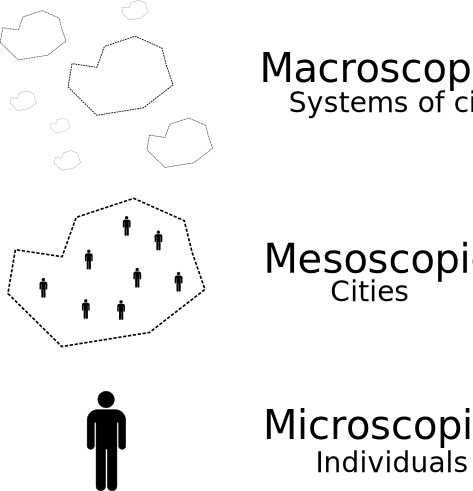
\includegraphics[width=\textwidth]{./gfx/chapter-intro/spatial_scales.pdf}
    \caption{{\bf Interactions at different spatial scales.} Cities are the
    result of interactions occuring at different spatial scales. The movement
and interactions of individuals result in the properties of the city as a whole.
But cities are not closed systems, and interact with other cities in a system of
cities.\label{fig:spatialscale}}
\end{figure}


Cities are therefore the result of interactions occuring at different spatial
scales. Furthemore, they are not static: they evolve in time, through various
processes taking place at different time scales.



\subsection{Time scales}
\label{ssub:time_scales}

First we have time-scales of the order of a day, which span the daily commuting
of inhabitants. This incessant movement of people has been traditionally
explored through surveys, but new data now allow more thorough studies. The
digital traces that are left by people at all times (through their mobile phone,
metro pass or GPS device) indeed allow us to explore the structure of flows and
the pace of life in cities at unprecedently fine spatial and time resolutions.

Then, at the order of a year one can see the variation in terms of wealth,
population, etc. of cities, as recorded by statistics agencies. Data about
demographic, social and economic aspects of urban systems allow us to
characterise more specifically the structure and behaviours of these systems.

Finally, at time scales of the order of ten years, we can see the city's
infrastructure as well as its spatial footprint evolve. The study of the
underlying processes is made possible by various projects lead by the GIS
community, historians and geographers which aim at digitizing historical maps of
the road and rail networks in different regions of the world. Also, since the
$1970s$, many satellites have been taking pictures of the Earth's surface, and
the remote sensing community has been treating these data to get information
about the spatial extension of cities. These data should give us some insight
about the processes responsible for the long-term evolution of cities's
structure.\\

\begin{figure}[!h]
    \centering
    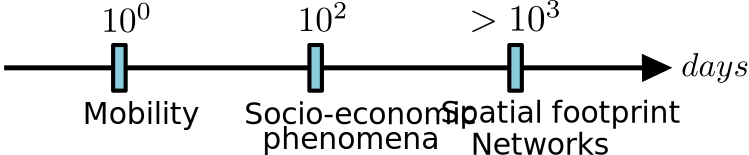
\includegraphics[width=0.9\textwidth]{./gfx/chapter-intro/time_scales.pdf}
    \caption{{\bf Different time scales.} The various data available about
    cities are associated with different time scales.\label{fig:timescale}}
\end{figure}

These time scales are summarised on Fig.~\ref{fig:timescale}. The long-term goal
of our studies is to understand exactly how cities and systems of cities behave,
and how interactions between these three layers lead to the behaviours we
observe. 

% Introduction

\pdfbookmark[1]{Quantitative revolutions}{Introduction}

\chapter{Quantitative revolution(s) in urban science}
\label{chap:quantitative_revolutions}

\begin{flushright}{\slshape    
And the first one now\\
Will later be last\\
For the times, they are a-changin'} \\ \medskip
--- Bob Dylan 
\end{flushright}


\bigskip


It is difficult to make a concise summary of what is known and not known about
urban systems. The vast amount of knowledge that has been gathered so far seems
very little in comparison to the bewildering complexity of the object being
studied~\cite{Batty:2008}. Every map, every satellite view, every statistic, every step
in cities elicits a question yet to be answered. What do we have to answer them?
A surprisingly small array of empirical tools and models. A surprisingly small
amount of solid, undisputed empirical facts.

Having said that, previous contributions are by no mean negligible. The body of
quantitative knowledge about cities has dramatically grown since the
quantitative revolution in Geography that took place after the $1950$s.
Recently, people have suggested that we may be witnessing the dawn of a second
quantitative revolution.\\

In the following Chapter, we will try to get some perspective on this claim, and
see to what extent it is justified. We will start with a (very) brief account of the
first quantitative revolution and the main themes around which it articulated
knowledge (a more comprehensive account can be found in~\cite{Sanders:2011}). We
will then critically review the factors traditionally invoked to justify the
spreading expression 'second quantitative revolution'.



\section{The first quantitative revolution}
\label{sec:the_first_quantitative_revolution}

Quantitative efforts in the study of human activities find their origin in Von
Th\"unen's model of agricultural land in $1826$, which suggests that the rent of land
should decay linearly with the distance to the city. More than a century later,
in $1933$, the German geographer Walter Christaller published his Central Place
Theory~\cite{Christaller:1933}, which aimed at explaining the size and location
of settlements in a system of cities. Needless to say, these early efforts are
theoretical in nature, and the empirical aspect -- studying things as they are
-- is left out. Surely due to the lack of available data.\\

The quantitative effort really starts to spread in the US in the
$1950$-$1960$~\cite{Berry:1993}. From the very beginning, the objective to make
geography a science is clearly stated. Starting with the introduction of Bunge's
seminal \emph{Theoretical Geography}, published in $1962$~\cite{Bunge:1962}.
According to the author, geographers can and should go beyond the mere
accumulation of facts, and try to discover the laws that rule the human and
physical phenomena occuring on the Earth's surface.   

Bunge proposed geometry as a tool to understand the observed pattern and
describe objectively the geographical space. The range of tools used quickly
expanded~\cite{Haggett:1966,Chorley:1968}, spanning stastistical
models~\cite{King:1969, Brunsdon:1998} -- whose importance is demonstrated by
the publication in $1969$ of Leslie King's \emph{Statistical Analysis in
geography}) -- and graph theory  -- as early as $1963$ with the publication of
Kansky's PhD thesis~\cite{Kansky:1963}. An early review of the use of graph
theory in geography can be found in Hagget and Chorley's
book~\cite{Haggett:1969}.\\

The research undertaken in the quantitative tradition can be -- tentatively --
divided in three different categories. First, the study of spatial
differentiation, aims at characterising the spatial patterns that result from
human activities. For instance, the study of population or employment densities
(see Part~\ref{part:polycentricity}), the local concentration of population
categories (see Part~\ref{part:segregation}), or the repartition of cities
inside a territory. 

Second, the study of spatial interactions. The progressive realisation that
distance is a critical factor to understand the arrangement of different spatial
phenomena led Tobler to state the First Law of Geography~\cite{Tobler:1970}. 

\begin{quote}
    Everything is related to everything else. But near things
    are more related than distant things.
\end{quote}

Linked to the study of spatial interactions is the (in)famous gravity model,
which states that the flow $F_{ij}$ between two locations $i$ and $j$ is given
by a function of the form

\begin{equation}
    F_{ij} = C\, P_i^\alpha\,P_j^\beta\, f(d_{ij})
\end{equation}

where $f$ is a decreasing function of distance. Although the analogy with
Newton's gravitation law was used by Reilly in $1931$ to find the retail market
boundaries between cities~\cite{Reilly:1931}, the above formulation in terms of
flows was formulated by Stewart in~\cite{Stewart:1948}. Note the competing
existence of Stouffer's theory of intervening
opportunities~\cite{Stouffer:1940}, according to which the flow between $i$ and
$j$ is proportional to the number of opportunities at $j$ and inversely
proportional to the number of opportunities between $i$ and $j$. It was
mathematically formulated later by Simini et al.~\cite{Simini:2012}.

Finally, the study of infrastructure. Starting with Kansky in
$1963$~\cite{Kansky:1963}, the study of the shape and growth of road networks,
railway networks and other infrastructure has witnessed a renewed interest
thanks to the study of spatial networks~\cite{Barthelemy:2011}.


\section{A second quantitative revolution?}
\label{sec:a_second_quantitative_revolution_}

People can be forgiven for believing that the present time bears any sort of
special character. But when we look closely enough, the change is perpetual, and
what is new now will be outdated tomorrow. During the past $3$ years, I have
at many times overheard the fact that we were currently witnessing a 'second
quantitative revolution' in the study of geographical systems. But is it really
the case? What differences with past tools or methods could justify such a
claim? In the following, we explore the three following hypotheses

\begin{itemize}
    \item The quantitative revolution is due to the availability of `new data';
    \item The quantitative revolution is due to the use of new methods coming
        from interdisciplinary studies;
    \item The new quantitative revolution is due to a technological convergence.      
\end{itemize}



\subsection{New methods}
\label{sub:new_methods}

The recent years have seen the application of new methods, mainly coming from
physics or computer science, to the study of cities. Either by geographers, or
outsiders who established well-established methods from another
field~\cite{Batty:1995}. These collaborations, or incursions, are however not
new. For instance, John Stewart, an american astrophysicists is famous for the first use of allometric
scaling in the study of cities~\cite{Stewart:1947}, or for his work 
on the gravitation model~\cite{Stewart:1948}. Another interesting example is
given by the collaboration in $1971$ between Waldo Tobler -- a geographer -- and
Leon Glass -- a chemist -- who plot the radial distribution function of Spanish
cities, a method that is traditionally used to study the property of
liquids~\cite{Glass:1971}.

So, the application of well-established methods from other fields to cities is
not new, and neither are the contributions made by outsiders. Yet, we can
identify two qualitative changes: the number, and nature of these contributions.
If some authors have continued to import directly methods and models from other
disciplines (for instance, the use of diffusion-limited aggregation models,
traditionally studied in physics, to explain the growth of
cities~\cite{Makse:1995}), this type of theoretical contribution is becoming
marginal. Contributions are more and more empirical; and if theoretical, are not
direct applications of another domain's theories. For
instance, Rozenfeld and co-authors used percolation on census tracts to define
cities~\cite{Rozenfeld:2008} in an original way. Masucci et al. use percolation
on the road network for the same purpose~\cite{Masucci:2015}, while Li et al.
use percolation to study the properties of congestion~\cite{Li:2015}. New
approaches to spatial network~\cite{Barthelemy:2011} have yielded new insights
into the structure and evolution of road, railway and subway networks~\cite{Strano:2012,
Barthelemy:2013,Louf:2013_emergence,Louf:2014_scaling,Louf:2014}.
Original out-of-equilibrium models that are inspired by the studied system allow
a better understanding: Simini's radiation model~\cite{Simini:2012,Simini:2013}
 -- which is nothing else that the mathematical transposition of Stouffer's
 intervening opportunities theory -- or our model to explain the polycentric
 transition of cities~\cite{Louf:2013_polycentric} are examples of such models.
 Not to forget the important literature on scaling
 relationships~\cite{Bettencourt:2007, Bettencourt:2013, Louf:2014_mobility,
 Arcaute:2014, Louf:2014_smog}, and other empirical analyses -- such as the
 study of residential segregation we present in Part~\cite{part:segregation}.
% Agent based model must be included somwehere here!

At the same time, the number of contributions to the field from authors who do
not have a geography (or economics, urbanism, etc. for that matter) has been
increasing over the pas years. After all, I am a theoretical physicist by
training, this thesis will be officially be registered as a theoretical physics
thesis. So, if the contributions of outsiders are not new, they are changing in
number and nature. To the point where we can wonder whether some of these
`outsiders' should still be considered as such.



    \subsection{New data?}
    \label{sub:new_data}

Population Mapping usinf mobile phone data~\cite{Deville:2014}
Lots of talks about new data, but I have used almost none during my thesis.
FourSquare~\cite{Noulas:2012}, Twitter... Credit cards~\cite{Lenormand:2015}

\begin{figure}
    \centering
    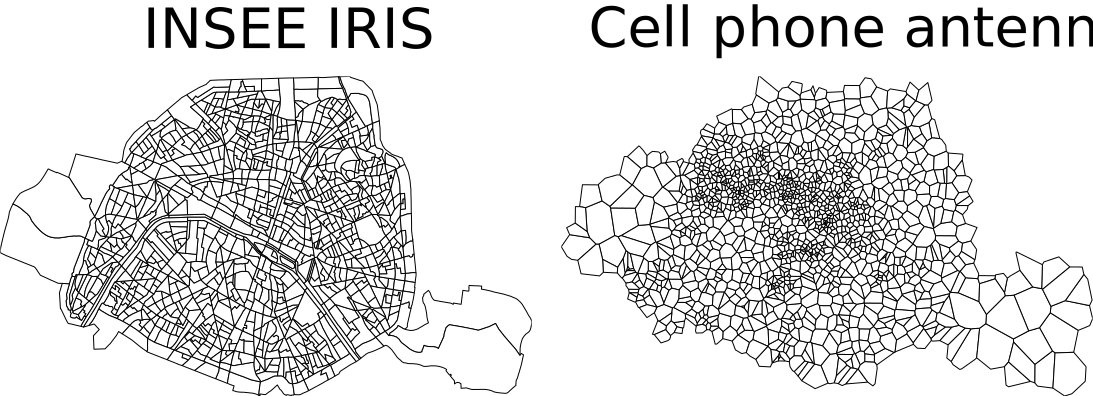
\includegraphics[width=\textwidth]{gfx/chapter-intro/IRIS_phone.pdf}
    \caption{(Left) IRIS zones in Paris, the smallest statistical units defined
    by the national statistics institute, INSEE. (Right) Voronoi tesselation
    built from the position of antennas of a popular french mobile phone carrier.
    There are $40\%$ more antennas than there are IRIS, and they tend to be more
    concentrated in zones of high daily activity (8th and 9th
    arrondissements).\label{fig:IRIS_phone}}
\end{figure}

Mobile phone data are spatially more precise. They give us a \emph{continuous}
information about the flow of individuals within the city, and not only
commuting.

But be careful. If they are ok to monitor aggregate
quantities~\cite{Lenormand:2014}, be careful of
individuals trajectories because sampled in a weird way.

    \subsection{A technological convergence}
    \label{sub:a_technological_convergence} 



Interdisciplinary collaborations already existed, data were already there. So
what is the qualitative difference between the state of the field say $20$ years
ago, and the state of the field as it is now, if any?\cite{Batty:2008,Batty:2012,Batty:2013} seeing the city as flows and networks.

\cite{Makse:1995} Modelling urban growth with diffusion limited aggregation
\cite{Rozenfeld:2008} Laws of population growth, using CCA algorithm to define
urban areas.


Agent-based models. Physicists have learned to be wary of the attempt to
describe in a deterministic framework the interactions of thousands, billions of
particles. Take a very simple model: the gas of hard spheres. Hard spheres are
simple objects: they have a fixed radius, cannot interpenetrate one another.
Their behaviour is well known, described by Newton's laws of motion, and we can
in theory solve all the equations describing their movements. In fact, we could
imagine, knowing the initial conditions, solve these equations and thus follow
the motion of every single particle (its position and speed) over time. In
practice, computers are way better than we are at doing that, and can easily follow for
us the trajectories of millions of spheres---I have coded that myself as a
student. So we have a very simple system, whose behaviour is perfectly known and
for which we can write exact dynamical equations, thus knowing perfectly its
time evolution at any arbitrary instant in the future. So what? What do we learn
from this simulated motion? What did we understand about the \emph{collective}
motion of spheres that we did not already know performing these simulations?
There is too much information for us to understand. In fact, there is as much
information in these simulations than there is in the original phenomenon, and
our understanding has not improved.
Facing the same questions, the fathers of statistical physics proposed to
extract some simpler, macroscopic information using probabilistic arguments.

Now, regarding social system, the context is even worse. We don't even know the
laws that determine the behaviour of individuals... we do not have the
equivalent of Newton's dynamics to describe the evolution of individuals in time
and their interactions. It is thus difficult what we would gain from simulating
the motions of thousands, millions of them using massive simulations. Even if
the laws were right, what would we learn from these simulations?

 % Chapter 1
% Introduction

\pdfbookmark[1]{Introduction}{Introduction}

\chapter{Methodology}
\label{chap:methodology}

\begin{flushright}{\slshape    
If it disagrees with experiment, it's wrong.\\ 
In that simple statement is the key to Science.} \\ \medskip
--- Richard Feynman~\cite{Feynman:1965}
\end{flushright}


\bigskip


\section{The importance of being naive}
\label{sec:the_importance_of_being_naive}

\section{In defense of reductionism}
\label{sec:in_defense_of_reductionism}

In fact, we do not need to have a full theoretical description of the human mind
to say something about the actions of hundreds of thousands, a million of them.
In the same way we do not need string theory in order to explain the
functioning of living organisms.

Randomness is not to be understood as the opposite of rationality. Individuals
may as well make perfectly rational, predictable decisions, we would still have
to use a probabilistic approach. Particles are an extreme example of individuals
with a rational behaviour, yet we describe their collective behaviour with
statistical physics. Probabilities are not called for by the unpredictability of
one's behaviour, but rather by the particular type of information that is
important to us -- and that we can process.

What tells us that the world is not more complex than the picture drawn by
physical theories? That our best theories are only approximations that work a t
a certain scale, but are plain wrong at others? Everything around us, and the
history of physics itself. Reductionism does not imply renouncing to the world
in its entirity and its complexity. Reductionism is merely a recognition of our
limited capabilities, our possibility to grasp only the world tiny bit by tiny
bit, approximation after approximation. It is not absurb to reduce the amount of
information that is dealt with in theories, because this seems to be exactly how
we are cognitively programmed to function. If our brains were able to embrace
the world in all its details at once, one wouldn't need models, one would not
need theories, one wouldn't need science. Observation would be synonymous 
understanding.\\
History of Physics tends to prove to us that, in fact, all theories \emph{are}
effective theories -- in the sense that they are only true at a given scale. Too
aproximate when our measufing apparatus are able to probe nature more into
details. The analogy here is clear: we need more data, more specific data first
if we want to dig deeper into the reality of our societies, economies. We need
more than our own eyes, more than our ears. We need social, economical
telescopes.

\section{Quantitative stands for 'data'}
\label{sec:quantitative_stands_for_data_}

Richard Feynman's statement used as an epigraph in this chapter might be an
oversimplified, narrow view of what Science is and how it proceeds. It
nevertheless hits the nail right in the head, by isolating the core component of
what Science is: a tight relation with empirical analysis.

\section{Against data}
\label{sec:against_data}

In `Againt Method', the philosopher of science Paul Feyerabend argued against
the idea that Science proceeds through the application of a single, monolithic
method; what people usually call `The Scientific Method'~\cite{Feyerabend:1975}.
The reference is not innocent, and I will argue here that, although empirical
analysis constitutes the alpha and the omega of our enquiry for knowledge, data
are not enough.
There is common confusion, often innocent, that because data are at the core of
scientific enquiry, one only needs data analysis to understand how a system
works and predict its behaviour -- especially so when we have a lot of data. An
very extreme view of this statement has recently been put forth by Big Data
supporters. An article in the magazine `Wired'~\cite{Anderson:2008} recently
argued that the current deluge of data marked the end of Science as we know it.
That models were not necessary anymore, that they were to be replace with the
extensive correlation analysis that a vast amount of data allow. This view is
completely misguided.\\

For one, pure data analysis is, at best, a myth: as Pierre Duhem argued in
$1906$~\cite{Duhem:1997}, all empirical observations are theory-laden. That is,
they are necessarily affected by the theoretical presuppositions held by whoever
is making the observation. Measuring the population of a city, for instance,
presupposes that there are such objects as cities, and that we can delineate
them. A deluge of data does not relieve the investigator from defining the
objects she is studying, from implicitely thinking about the relation between
the different elements in the system.

Then, correlations are science, indeed. But they are rudimentary science, and
there is nothing new about them. Arguably, the reason why we are able to
function at all as individuals is because our brain is capable of computing
correlations all the time. Take chairs. Chairs are fairly simple objects. Yet,
they come in all kind of colors, material and shapes. And despite this
potentially infinte diversity, I am able to recognise a chair when I see one. I
also have a notion of what a chair is to be used for. Although we do not
ackowledge it often, we are capable of surprisingly high levels of abstraction
and generalisation. Because we correlate, all the time. Science starts with the
observation of these regularities. For instance, that the sun always appears at
the same place and disappears in the opposite directions. That seasons come and
go regularly. That after the night always comes the day. Is it useful? Yes, for
limited applications. Does it make it science? No. Science is when one goes
beyond the simple observation of correlations, and tries to write down a model,
to understand the mechanisms responsible for the correlations we observe.\\

Data is not enough, we must build model, theories.

\section{An example: The law of metropolises}
\label{sec:an_example_the_law_of_metropolises}

\subsection{Statement}
\label{sub:statement}

The above discourse may seem a bit abstract (maybe because it is?), so let us
see the shortcomings of pure data analysis on a simple example, related to
cities.

Using the GEOPOLIS database, Moriconi-Ebrard derived a general transversal rule about system
of cities, that he called \emph{law of metropolises}~\cite{Pumain:1997}. If we
note $P_U$ the urban population of systems of cities, and $P_1$ the size of
their largest city~\graffito{The original regularity was observed for what the
author calls 'metropolises', which are roughly equivalent to the largest city in
terms of population.}, we can
plot $P_1$ versus $P_U$ for all systems of cities and obtain the plot on
Figure~\ref{fig:metropolises}.

\begin{figure}[!h]
    \centering
    \includegraphics[width=\textwidth]{gfx/chapter-intro/law_metropolises.pdf}
    \caption{{\bf The law of metropolises.} Population of the largest city of
    systems of cities $P_1$ versus the total urban population $P_u$ in that
system. The dashed line shows the result of a powerlaw fit, whose exponent
agrees well with the one found in~\cite{Pumain:1997}. Data for the total urban
population and the population of the largest city of countries in the year
$2000$ were obtained from
the World Bank.\label{fig:metropolises}}
\end{figure}

Assuming a powerlaw relationship between the two quantities, one finds

\begin{equation}
    P_1 \sim P_U^{\,0.84}\:(r^2=0.98)
    \label{eq:metropolis}
\end{equation}

which agrees very well with the empirical data (for all years where data are
available). It is tempting, at first, to consider this as yet-another emprical
regularity exhibited by urban systems, and try to find a coherent interpretation
in geographical terms. However, as we will show, if we assume that the Auerbach-Zipf
law~\cite{Auerbach:1913,Zipf:1949} holds for each system of cities
individually

\begin{enumerate}
    \item We can derive a relation that fits the data as well as
        Eq.~\ref{eq:metropolis};
    \item The relation is not a powerlaw.
\end{enumerate}



\subsection{Deriving the `law of metropolises'}
\label{sub:deriving_the_law_of_metropolises_}

Let us consider a system of cities comprised of $N$ cities, with total
population $P_U$. The size of the largest city is noted $P_1$. We assume that
the distribution of city sizes follows the Auerbach-Zipf law, so that the city
of rank $r$ (the $r$th largest city) has a population

\begin{equation*}
    P_r = P_1\,r^{-\mu}
\end{equation*}

So the total population in the system of cities can be written

\begin{equation}
    P_U = \sum_{r=1}^N P_r = P_1\,\sum_{r=1}^{N} \frac{1}{r^\mu}
\end{equation}

If we assume that $\mu=1$, $P_U$ is given by the harmonic series, and thus

\begin{equation}
    P_U = P_1 \left[ \ln(N) + \gamma + O\left(\frac{1}{N}\right)\right]
\end{equation}

where $\gamma \approx 2.58$ is Euler's constant. This gives us a first relation
between $P_1$, $P_U$ and $N$.\\

Still using the assumption that the distribution of city size follows the
Auerbach-Zipf law with $\mu=1$, we can show (using extremal value
theory)~\cite{Clauset:2009} that on average\graffito{'Average' as in {\bf
ensemble average}} the size of the largest city is proportional to the total
number of cities

\begin{equation*}
    P_1 \propto N
\end{equation*}

Thus, when the number of cities in the system is large, $N \gg 1$ the following
relation holds 

\begin{equation}
    \boxed{P_1\,\ln(P_1) = P_U}
    \label{eq:metropolises_debunked}
\end{equation}

As one can see on Figure\ref{fig:metropolises_debunked}, the formula given by
Eq.~\ref{eq:metropolises_debunked} fit the data as well as the previous one.

\begin{figure}[!h]
    \centering
    \includegraphics[width=\textwidth]{gfx/chapter-intro/law_metropolises_debunked.pdf}
    \caption{{\bf The law of metropolises revisted.} $P_1 \ln(P_1)$ versus the total urban population $P_u$ in that
system. The dashed line shows the result of a linear fit, which agrees as well
with the data as does the powerlaw relation assumed in~\cite{Pumain:1997}. Data for the total urban
population and the population of the largest city of countries in the year
$2000$ were obtained from
the World Bank.\label{fig:metropolises_debunked}}
\end{figure}


It is therefore impossible to determine which of
Eq.~\ref{eq:metropolises} of Eq.~\ref{eq:metropolises_debunked} describes the
`true' relation between $P_1$ and $P_U$ based on data analysis alone.
Nevertheless, the later finds a very simple explanation in the fact that cities
in systems of cities follow the Zipf-Auerbach law up to a good
approximation. In the absence of any theoretical explanation for the powerlaw
relationship and given the empirical equivalence of both forms, it
least-assuming to consider $P_1 \ln P_1 \sim P_u$.


\subsection{Lessons learned}
\label{sub:lessons_learned}

So, not only is the \emph{law of metropolises} not a fundamental relation, it is
rigorously wrong. 

This teaches us that, given the range of variations of the measured
quantities, it is very difficult to distinguish empirically a powerlaw
relationship from something qualitatively different such as $Y \ln Y \sim P$.
One should therefore be wary of interpreting empirical relationships,
like the one originally found in~\cite{Pumain:1987}, unless a mechanistic
explanation of the fitted relationship is provided. As a matter of fact, what
was thought as a fundamental law might end up being trivial and without great
interest.

We will discuss this matter again in Chapter~\cite{chap:scaling-implications} when
discussing the conclusions we can draw from the analysis of scaling
relationships. But before doing so, we need to talk about models and theories.


\section{Of models and theories}

\subsection{Why bother?}
\label{sub:why_bother_}

As scientific sceptics often like to remind us, all models, all theories are
wrong. But surely, there must be some interest in models to make them deserve
the months, sometimes years of work that scientist devote to them. Admittedly,
many take for granted the usefulness for model, or it seems so obvious that they
never question their quest.

The models two main functions are , broadly speaking, to understand, and to
predict.  The notion of simplification is close to the notion of `mental
economy' defended by the Philosopher of Science Ernst Mach.  According to him,
models' main function is to allow us to condense an infinity of possible
situations in very compact descriptions. Take Snell's law of refraction between
two media of optical indices $n_1$ and $n_2$

\begin{equation}
    n_1\,\sin \theta_1 = n_2\,\sin \theta_2
\end{equation}

In a single formula are contained an infinite number of possible experimental
configurations. Through this model, we are able

This picture is obviously incomplete. Some models obviously do not aim at being
correct from the beginning.

\subsection{Theory, not analogy}
\label{sub:theory_not_analogy}




There are two issues with the current state of affair 
Fancy words are too often used as a substitute for a real
understanding of the system. But, however intellectually appealing they are,
metaphors are not a theory. What do we understand from the comparison of cities
with biological systems? What new knowledge do we gain? Sure, the most important
ideas are those that you trigger, but you are responsible for the way your ideas
are interpreted.  Maybe cities are an easy pray for this sort of behaviour.
Since there is very little understandin, and the immediacy, complexity and
diversity of out experiences with cities creates this big gap in which anyone
can slip an idea or two, that will be interpreted in very different ways by
different people. The genius of metaphors is not to provide interesting ideas
that are ready to be applied to a specific fiedld. Rather, it is to trigger very
different ideas into different people. But this when we should realise the power
of the metaphor and leave it behind, following the trail of the new ideas thus
triggered. What we need to highlight are regularities, not similarities.

What is wrong, and somwehat uncomfortable in the present literature, is the
impression that models and reality live in two distinct, very loosely connected
worlds. Often, the gap is bridged through some intellectual trick, be it analogy
or metaphor.

A very nice quote is the beginning of the EPR paper

In the following manuscript, I will therefore pay a special attention to the
rigour in the language used. Qualify suggestions, by presenting them as such.
This kind of work may be less suggestive, the vocabulary used less expressive,
it may not make the reader feel as good about herself, but it is a necessary
step towards a science of cities. We need to clear the language of unfruitful
metaphors and fill the gap with mechanisms.

% Introduction

\pdfbookmark[1]{Methodology}{Methodology}

\chapter{About this thesis}
\label{chap:methodology}

%\begin{flushright}{\slshape    
%In the long run men only hit what they aim at.\\
%Therefore, though they should fail immediately\\
%they had better aim at something high.} \\ \medskip
%--- Henry David Thoreau
%\end{flushright}

\begin{flushright}{\slshape    
Anybody can plan weird, that's easy.} \\ \medskip
--- Charles Mingus
\end{flushright}


\bigskip 


The following thesis might surprise the reader used to the monographs usually
produced by PhD students in Social Sciences, articulated around a single,
general question. The outline of this thesis reflects more the
line of thoughts and of research that has been undertaken than the answer to a
single question that would have been asked a priori and answered during the
last three years. For that reason, the four Parts of this thesis are mostly
independent. There is not single thread holding them together. But rather multiple
wires; common themes and similar ideas. 

\section{Outline}

Part~\ref{part:polycentricity} tackles the problem of measuring and
understanding urban form, an issue that has been running through the $3$ years
of my PhD. In this Part, we first (Chapter~\ref{chap:monocentric_introduction})
present a brief historical overview of the monocentric and polycentric
representation of the city, before enumerating the methods that are used in the
literature to count the number of activity centers. We end with the observation
that the number of activity centers increases in a regular way with population
size. The following chapter (Chapter~\ref{chap:monocentric_model}) is devoted to
an out-of-equilibrium model that we built in order to explain the previous
empirical regularity. The model is able to predict the sublinear increase of the
number of centers that we observe on American and Spanish data. In the last
chapter (Chapter~\ref{chap:monocentric_discussion}), we question the assumptions
of the model and the current empirical methods to quantify urban form.\\

Part~\ref{part:scaling} is concerned with scaling relationships. We first propose
(Chapter~\ref{chap:scaling_introduction}) a non-exhaustive overview of the dawn
and surge of allometric scalings, from Stewart's $1949$ to the recent wealth of
studies. Then, using the model developped in the preceding part, we show in
Chapter~\ref{chap:scaling_model} how the structure of mobility patterns allow us
to understand the qualitative and quantitative values of the exponents related
to urban form and mobility. We conclude this part with a discussion on the
interpretation of these scaling laws, and their important shortcomings
(Chapter~\ref{chap:scaling_implications}).\\

Part~\ref{part:segregation} departs from the preceding chapters and turns to the
study of residential segregation. Driven by the desire to extend the model
presented in Chapter~\ref{chap:monocentric_model}, we soon realised there was a
lack of robust empirical description of patterns of segregation that could be
reproduced by a model. In Chapter~\ref{chap:segregation_introduction} we tackle
the problem of defining what segregation is; we propose a brief review of the
existing literature, and subsequently define a null model -- the segregated
city. In the next Chapter (Chapter~\ref{chap:patterns_segregation}), we build on
this null model to propose a set of measures to quantify patterns of residential
segregation.\\

Part~\ref{part:networks} concerns the original topic of this thesis: spatial
networks. Because my interests have shifted towards the study of
socio-economical phenomena over the years, we only briefly present the most
important results in the present thesis. We first (Chapter~\ref{chap:typology}) present an empirical
study of $131$ street patterns across the world where we propose a method to
classify the patterns based on the geometrical shape of the blocks. In the
following chapter (Chapter~\ref{chap:cost-benefit}), we present a cost-benefit
analysis framework to understand the properties and growth of spatial networks.
We introduce an iterative model that can explain the emergence of a hierarchical
structure (`hubs and spokes') in growing spatial networks. Starting from the
cost-benefit framework of this model, we show that the length, number of
stations and ridership of subways and rail networks can be estimated knowing the
area, population and wealth of the underlying region.\\

Finally, Part~\ref{part:conclusion} ties everything together, highlights the lessons
learned and concludes this thesis with some potentially interesting research avenues for the
years to come.



\section{Miscellaneous notes}

\subsection{Style}
\label{sub:style}

I will be using the pronoun 'we' for most of the manuscript, to reflect the fact
that the work presented here was, for the most part, done in the context of
collaboration with others. For the sake of clarity, the technical details of
calculations have been omitted in this manuscript. Most of these calculations are
relatively simple anyway, and the interested reader can find them in the
publications mentioned on page~\ref{p:publications} of this manuscript.

\subsection{Tools}
\label{sub:tools}

Unless otherwise specified, all figures in this manuscript have been prepared
using Python $2.7$~\footnote{Available at \url{http://www.python.org}} and the
Matplotlib library~\cite{Hunter:2007}. Inkscape~\footnote{Available at
\url{https://inkscape.org/en/}} was used to prepare most diagrams. This document
was typeset using Vim and \LaTeX. The template used is the typographical look-and-feel
\texttt{classicthesis} developed by Andr\'e
Miede.\footnote{Available at 
\url{http://code.google.com/p/classicthesis/}.}

\begin{center}
\end{center}


\cleardoublepage % Empty page before the start of the next part

%------------------------------------------------

\ctparttext{

The monocentric model of cities -- where all activities are organised around a
single activity center -- has pervaded the literature on urban systems for more
than $4$ decades. However, as it was repeatedly demonstrated, the model is empirically
inadequate.

The contribution of this part is threefold. First, we trace the history of ideas
regarding urban form, from the monocentric hypothesis and its origins, to the
various methods proposed to identify and count subcenters. We then demonstrate
empirically the existence of a polycentric transition for cities, and that the
number of centers increases as a sublinear function of the population size of
cities. Finally, we propose an out-of-equilibrium model that explains the
emergence of new subcenters as cities expand, and predicts the sublinear
increase of the number of centers with population size.

}

\part{Polycentri-city}
\label{part:polycentricity}

% !TEX root = ../thesis-example.tex
%
\chapter{The (end of the) monocentric city}
\label{sec:related}


\section{Introduction}
\label{sec:introduction}

[Picture 3D? of employment density profiles of different cities]

The problem with the traditional models of cities in two pictures: the
(polycentric) reality and the AMM model.


Alonso-Muth-Mills model might be the reason for the long-lasting influence of
the monocentric model (nice exposition in~\cite{Fujita:1989}).

\cite{Mills:1972} is a monograph discussing the causes of decentralisation and
suburbanisation. [could not read]

\cite{Kemper:1974} explores data trying to fit a negative exponential function
to industry and employment density. It does not work so well.

\cite{Odland:1978} explores the possibility of polycentric cities on a
theoretical basis. [could not read]

\cite{Griffith:1981} tool to evaluate the polycentricity of a pattern.[could not
read]

Treatment of the polycentric city in the urban economics literature starts
with~\cite{Fujita:1982}.

\cite{Dokmeci:1994} shows that Istanbul's employment is spread across several
centers. Although there is still a lack of strong quantitative evidence, the
idea is gaining ground.



\section{How to measure polycentrity}
\label{sec:how_to_measure_polycentrity}

\cite{McDonald:1987} proposes the first empirical method to identify employment
subcenters.

\cite{Giuliano:1991} uses an arbitrary threshold to determine the centers.

\cite{Anas:1998} Critices the method of Giuliano, has a cool picture of
Los-Angeles spreading and deals with urban structure.

\cite{McMillen:2001} proposes a non-parametric method to find the subcenters.

\cite{McMillen:2003} proposes a pretty good literature review in introduction on
the identification of employment subcenters, and proposes congestion as a reason
for the polycentric transition.

\cite{Tsai:2005} is a classic.

\cite{Griffith:2007} is yet another reference on spatial regression.

\cite{Pereira:2013} proposes an Urban Centrality Index that varies continuously
between a monocentric configuration and an extreme decentralized situation.

\cite{Louf:2013_polycentric} Proposes to use a property of the rank plot of the
employment density, exponential decrease.

\cite{Louail:2014} proposes a generalisation of the previous method based on the
Lorenz curve.

\cite{LeNechet:2015} a more recent paper.

I propose a generalisation, based on the same hypothesis but that is more robust
than the computation of the tangent at the origin.

\chapter{How congestion shapes cities}
\label{chap:monocentric_model}

We saw in chapter~\ref{chap:monocentric_intro} that as cities grow and expand,
they evolve from a monocentric organisation where all the activities are
concentrated in the same geographical area --usually the central business
district-- to a more distributed, polycentric organisation. We begin the
following chapter with introducing briefly the model of Fujita and Ogawa, in
urban economics, that allegedly explains the polycentric structure in cities. We
will highlight the issues of this model, before present our model inspired by
it. This model is a stochastic, out-of-equilibrium model and relies on the
assumption that the polycentric structure of large cities might find its origin
in congestion, irrespective of the particular local economic details. We are
able to reproduce many stylized facts, and --most importantly-- to derive a
general relation between the number of activity centers of a city and its
population. 


\section{Fujita and Ogawa}
\label{sec:fujita_and_ogawa}

In line with the tradition of economic geography~\cite{Fujita:2001}, the model
of Fujita and Ogawa~\cite{Fujita:1982} is based on the concept of agglomeration
economies---to explain why economical activities tend to group---and the spatial
distribution of wages and rents across the urban space. They consider that
cities are constituted of two kinds of actors: the firms, who tend to
concentrate to maximise their production, and the households, who try to
minimise their rent and commuting cost. In the following, I will present the
model, focusing on the hypotheses.\\ 

The model is \emph{static}, in the sense that the number of firms and
individuals are fixed. It is an \emph{equilibrium} model, considering the the
city is the realisation of a general optimum. The original model is also
\emph{one-dimensional}, although the hypothesis of one-dimensionality is not
fundamental, and only necessary to make the calculations easier. Because I will
not try to solve the model, I will write equations in the 2D case.

\subsection{Households} 
\label{sub:households}

Fujita and Ogawa assume that there is a fixed number $N$ of households in the
city. The households are considered identical, in the sense that they all have
the same utility function and the same budget constraint. The utility function
of each household is given by the function $U = U(Z)$ where $Z$ is the surplus
of money that is left after budgetary constraints (expressed in monetary units).
Basically the money one has left at the end of the month, once the rent, bills
and petrol (or transportation card) are paid. 

The utility is assumed to be an increasing function of $Z$ so

\begin{equation}
    \frac{\partial U}{\partial Z} > 0
\end{equation}

The budget constraint on an household living at $i$ (of coordinates $\vec{x}$)
and working at the firm located at $j$ (of coordinates $\vec{y}$) is given by the
equation

\begin{equation}
    Z = W\left(j\right)
      - C_R\left(i\right)
      - C_T\left(i,j\right)
\end{equation} 

where $W\left(j\right)$ is the wage earned at $j$, $C_R\left(i\right)$ the total
rent paid at $i$ and $C_T\left(i,j\right)$ the cost of commuting between
home and work. This equation is very general, and will be our starting point for
the model presented in the next section. The authors of~\cite{Fujita:1982}
further specify the commuting cost

\begin{equation}
    C_T\left(i,j\right) = t\,d_E(i,j) = t\,\left|\vec{y}-\vec{x}\right|
\end{equation}

where $t$ the commuting cost per unit distance, and $d_E(i,j) = \left| \vec{y} -
\vec{x} \right|$ the euclidean distance between home and work. The total rent
cost is further written as

\begin{equation}
    C_R\left(i\right) = R(i)\,S_h
\end{equation}

where $R(i)$ is the rent per unit surface at $i$, and $S_h$ the surface area
used by households, which becomes a parameter of the model.
The surplus $Z$
finally reads

\begin{equation}
    Z = W\left(j\right)
      - R\left(i\right)\,S_h
      - t\,d_E\left(i,j\right)
\end{equation} 


\subsection{Firms}
\label{sub:firms}

The second type of agents taken into consideration in the model are the firms.
It is assumed that all firms employ the same number of individuals, which
amounts to having a fixed number of firm $M$ (once the number of households is
fixed). The profit earned by a firm  located at $j$ reads, in a general
form

\begin{equation}
    \Pi = G\left(j\right) 
        - C_R\left(j\right) 
        -  W\left(j\right)\,L_f
\end{equation}

where $G$ is the total gain realised by the firm selling its production, $C_R$
the rent paid by the firm, and $L_f$ the total number of employees per firm---a
paramter of the model.\\

To take agglomeration economies into account, Fujita and Ogawa define the
locational potential $F$ defined by

\begin{equation}
    F\left(j\right) = \int_{\mathcal{C}} b(\vec{x})\,e^{-\alpha\,\left|\vec{y}-\vec{x}\right|}\:\mathrm{d}\vec{x}
\end{equation}

where $b(\vec{x})$ is the density of firms at $\vec{x}$. The integral runs over
the entire city's spatial extent $\mathcal{C}$. One can easily see that the
higher the density of firms in a radius of $1/\alpha$ around a firm, the higher
the locational potential is going to be. Balanced by the constraint imposed by
the rent, which prevents too many firms from agglomerating at the same location,
the locational potential likely is the term responsible for the existence of
polycentric solutions in the model. Indeed,the authors further write the total
gain $G$ as a multiple of $F$:

\begin{equation}
    G(j) = \beta\,F(j)
\end{equation}

where $\beta$ integrates both the productivity of the employees and the effect
of the locational potential. The rent, as
in the case of households, is written $C_R(j) = R(j)\,S_f$ where $S_f$, the
surface needed by firms, is a parameter of the model. The profit
of companies therefore reads

\begin{equation}
    \Pi = \beta\, \int_{\mathcal{C}} b(\vec{x})\,e^{-\alpha\,\left|\vec{y}-\vec{x}\right|}\:\mathrm{d}\vec{x}
        - R\left(j\right)\,S_f
        - W\left(j\right)
\end{equation}


\subsection{Equilibrium conditions and results}
\label{sub:equilibrium_conditions}

Once the budget constraints have been explicited, one needs to further define
the equilibrium conditions to be able to solve the model. First, the goal of
each household is to maximise their utility under the budget constraint.\\

[Explicit calculations here]\\

In other words, the maximisation of utility under budget constraints is
equivalent to chosing the residential location $i$ and the job location $j$ so
as to maximise $Z$. In other words, the maximisation of utility in this
particular is equivalent to performing a cost-benefit analysis. The firms have
no utility function, and choose to be a the location $j$ that maximises their
profit.\\

A further constraint is given by the bid-rent curve and goes as follows. The authors define two intermediate functions, $\Psi(\vec{x})$ and $\Phi(\vec{x})$ which are
respectively the bid rent function of households and of firms, defined as

\begin{align}
    \Psi\left(\vec{x}\right) &= \max_{\vec{x}} \left\{ \frac{1}{S_h} \left[W(\vec{x} ) - Z -
    t\,d_E\left(\vec{x}-\vec{y}\right)\right] | U(Z)\right\}\\
    \Phi\left(\vec{x}\right) &= \frac{1}{S_f} \left[\beta\,F(\vec{y}) - \Pi -
W(\vec{y})\right]
\end{align}

$\Psi(\vec{x})$ represents the maximum rent that the households could pay to be
located at $\vec{x}$ while still having a utility value $U$. $\Phi(\vec{y})$ is
the maximum rent that firms could pay to be located at $\vec{y}$. At
equilibrium, it is assumed that whoever's bid rent function is maximum at
$\vec{x}$ will be located at $\vec{x}$.\\

The results of this model, given its intricacy, are somewhat disapointing.
Unsurprisingly, the authors are not able to derive an analytical solution for
their model. What they do, however, is deriving the conditions on the parameters
for the existence of monocentric and polycentric organisations of activities,
using numerical methods.

\section{Problems with the Fujita and Ogawa model}
\label{sec:problems_with_the_fujita_and_ogawa_model}

This approach fails at giving a satisfactory quantitative account  of the
polycentric transition of cities. A lot can be said about the details of the
model and its assumptions. We choose here to only discuss the issues that we
feel are the most important, and that we will try to adress in our model. 

\paragraph{It is an equilibrium model.} In line with the rest of Urban
Economics~\cite{Fujita:2001, Fujita:2013}, they describe a city as being in
an equilibrium characterised by static spatial distributions of households and
business firms. However, the equilibrium assumption is unsupported as cities are
out-of-equilibrium systems and their dynamics is of particular interest for
practical applications~\cite{Batty:2008}.\\

\paragraph{It is too complex.} It integrates so many interactions and
variables that it is difficult to understand the hierarchy of processes
governing the evolution of cities, which ones are fundamental and which ones a
irrelevant. A model is only interesting when it
provides a simple structure to understand empirical results, whether it
reproduces them, or provides well-understood limiting case.\graffito{Limiting
case models are often called `null models'} 

\paragraph{It does not make any prediction.} Worse, due to its complexity, the
model is unsolvable, and does not make any prediction. At best it shows that
polycentric configurations are \emph{possible}. Yet, there are possibly different
models[possibly? Loo
at literature in economics] that admit polycentric activity profiles as a
solution. The model is thefore unsupported by data.\\ 

We also note that the model does not take the congestion into account in the
commuting cost (which is only a function of the distance). However, it is
mentioned in the economics literature as being a possible cause of the
polycentric transition of cities~\cite{McMillen:2003}. 

\section{Modeling the polycentric transition}
\label{sec:an_out_of_equilibrium_model_}

Following recent interdisciplinary efforts to construct a quantitative
description of cities and their
evolution~\cite{Makse:1995,Zanette:1997,Marsili:1998a,Marsili:1998b,Batty:book2005,Bettencourt:2007,Batty:2008},
we deliberately omit certain details and focus instead on basic processes. We
thereby aim at building a minimal model which captures the complexity of the
system and is able to account for --qualitative as well as quantitive-- stylized
facts. 
The model we propose is by essence dynamical and describes the evolution
of cities' organisation as their population increases. We focus on car
congestion -- mainly due to journey-to-work commutes -- and its effect on the job
location choice for individuals.\\

\subsection{Decoupling the choice of household and job}
\label{sub:decoupling_the_choice_of_household_and_job}

The time scales involved in the evolution of cities are usually such that the
employment turnover rate is larger than the relocation rate of households. On a
short time scale, we can thus focus on the process of job-seeking alone, leaving
aside the problem of the choice of residence. In other words, we assume the
coupling between both processes to be negligible: we assume that each inhabitant
newly added to the city has a random residence location and we concentrate on
understanding how such an inhabitant chooses its job location.\\

As a result of this assumptions, a worker living at $i$
will choose to work at the center $j$ such that the quantity
 
\begin{equation}
    Z_{ij} = W(j) - C_T(i,j)
    \label{eq:Z_workers_general}
\end{equation}

is maximum. Doing so, we give up any hope to describe the spatial structure of the rent
distribution, or the alledged scaling between rent prices and population size in
cities.

\subsection{Decoupling the dynamics of residence and work locations}
\label{sub:decoupling_the_dynamics_of_}

Another difficulty with the Fujita-Ogawa model is the strong coupling between
the behaviour of firms and individuals. The empirical literature on the
behaviour of firms points to a tendency of similar industries to cluster
geographically~\cite{Marcon:2003, Duranton:2005, Marcon:2009}, and a higher
profit of industries located in Urban environments~\cite{Melo:2009}. Although
theoretical attempts at explaining these behaviours have been
proposed~\cite{Duranton:2004}, the models are yet to be developped in an
out-of-equilibrium framework.\\

Here, we decide to simplify the problem by assuming that firms indeed cluster
into specific locations, that we call activity centers. Each worker can then
choose among a pool of $N_c$ potential activity centers (which we suppose are
also randomly distributed among the city). The active subcenters are then
defined as the subset of potential centers which have a non zero incoming number
of individuals. We thus assume that the existence of activity centers is defined
by the willingness of workers to work in the possible locations.\\


We now discuss the form of the wage $W(j)$ and the commuting cost $C_T$ that are
present in equation~\ref{eq:Z_workers_general}. 

\subsection{Determining the wage}
\label{sub:determining_the_wage}

The problem of determining the (spatial) variations of the average wage $W(j)$
at location $j$ is very reminiscent of some problems encountered in fundamental
physics. Indeed, the wage depends on many different factors, ranging from the
type of company, the education level of the inhabitant, the level of
aglomeration, etc., and in this respect is not too different from quantities
that can be measured in a large atom made of a large number of interacting
particles. In this situation, physicists found out that although it is possible
to write down the corresponding equations, not only is it impossible to solve
them, but also not really useful. In fact they found out~\cite{Dyson:1962} that
a statistical description of these systems, relying on random matrices could
lead to predictions which agree with experimental results.\\

We wish to import in spatial economics this idea of replacing a complex quantity
such as wages --which depends on so many factors and interactions-- by a random
one. The problem is not so much that we cannot write down the equations that
determine the wage that an individual could get in a given company. Even if we
could, the sheer number of people living in a urban area would surely prevent us
from solving these equations. And even if we could solve them, the resulting
information would be too overwhelming to really allow us to understand the
large-scale behaviour of the system as a whole. We thus need an \emph{effective}
theory of cities.
We therefore decide to account for the interaction between activity centers
and people by taking the wage as proportional to a random variable $\eta_j \in
\left[ 0,1\right]$ such that $W(j) = s\, \eta_j$ where $s$ defines the maximum
attainable average wage in the considered city.\\

We are aware that wages are not determined endogeneously but is rather the
result of thousands, millions of interactions between firms and individuals. In
the same way that Dyson did not mean that the interactions between electrons in
large atoms \emph{are} random, our assumptions does not mean that wages are
intrisincally randomly determined. What we mean, however, is that in the case of
systems containing a large number of individuals, one may possibly do \emph{as
if} they were randomly determined. Although we thereby abandon the possibility
to describe the dynamics of the wage distribution and the spatial 

\subsection{Commuting cost and congestion}
\label{sub:the_commuting_cost}


As for the transportation cost $C_T(i,j)$, we choose it to be
proportional to the commuting time between $i$ and $j$. In a typical
situation where passenger transportation is dominated by personal
vehicles, this commuting time not only depends on the distance between
the two places, but also on the traffic between $i$ and $j$, the vehicle capacity of
the underlying network and its resilience to congestion. The Bureau of
Public Road formula~\cite{Branston:1976} proposes a simple form taking
all these ingredients into account. In our framework, it leads to the following expression for the 
commuting costs

\begin{equation}
    C_T(i,j) =  t\, d_{ij} \left[ 1 + \left( \frac{T_{ij}}{c} \right)^{\mu} \right]
    \label{eq:commuting_cost}
\end{equation}

where $T_{ij}$ the trafic per unit of time between $i$ and $j$ and $c$
is the typical capacity of a road (taken constant here). The quantity
$\mu$ is a parameter quantifying the resilience of the transportation
network to congestion. We further simplify the problem by assuming
than the traffic $T_{ij}$ is only a function of the subcenter $j$ and
therefore write $T_{ij}=T(j)$ the total traffic incoming in subcenter
$j$ (see Supplementary Material~\cite{SM} for a short discussion).

\subsection{Summary}
\label{sub:summary}


In summary, our model is defined as follows. At each time step, we add
a new individual $i$ located at random in the city, who will
choose to work in the activity area $j$ (among $N_c$ possibilities
located at random) such that the following quantity
%
\begin{equation}
Z_{ij} = \eta_j - \frac{d_{ij}}{\ell} \left[ 1 + \left( \frac{T(j)}{c} \right)^{\mu} \right]
\label{eq:cost_function}
\end{equation}
%
is maximum (we omitted irrelevant multiplicative factors). The quantity $\ell = s/t$ is interpreted as the maximum effective
commuting distance that people can financially withstand. 

\subsection{Monocentric to polycentric transition}
\label{sub:monocentric_to_polycentric_transition}

Depending on the relative importance of wages, distance and congestion, the
model predicts the existence of three different regimes: the monocentric regime
(top left Fig.~\ref{fig:model_results}), the distance-driven polycentric (top
right Fig.~\ref{fig:model_results}) regime and the attractivity-driven
polycentric (bottom Fig.~\ref{fig:model_results}) regime. 


\begin{figure}
    \centering
    \includegraphics[width=0.49\textwidth]{gfx/chapter-monocentric/1.pdf}
    \includegraphics[width=0.49\textwidth]{gfx/chapter-monocentric/2.pdf}
    \includegraphics[width=0.49\textwidth]{gfx/chapter-monocentric/3.pdf}
    \caption{The monocentric (top left), distance-driven polycentric (top right)
      and attractivity-driven polycentric (bottom) regimes as produced by
      our model. Each link represents a commuting journey to an activity center. \label{fig:model_results}}
\end{figure}

The existence of a monocentric regime depends on how $\ell$---the maximum commuting distance that people can
afford--- compares to the size of the city $L$. Indeed, it is easy to
see that people located at a distance $d_{ij} > \ell$
from the most attractive center will not be able to afford commuting to this
center, and will, according to our model, choose to commute to a closer center.
As a result, a monocentric regime is only sustainable as long as people's
residence is drawn close to the most attractive center. In the limit where $\ell
\gg L$, the attractiveness of a center becomes irrelevant, and a monocentric regime cannot
exist. In these cases, we end up in the situation shown on the top-right of
Fig.~\ref{fig:model_results}.\\


From now on, we will assume that $\ell$ is large enough so that a
monocentric state exists for small values of the population. In this
regime, the value of $\eta$ prevails and the monocentric state evolves
to an attractivity-driven polycentric structure as the population
increases. 
Starting from a small city with a monocentric
organisation, the traffic is negligible and 

$$Z_{ij}\approx \eta_j$$

which implies that all individual are going to choose the most attractive
center, that is the center with the largest value of $\eta_j$, say $\eta_1$.
When the number $P$ of households increases, the traffic will also increase and
some initially less attractive centers (with smaller values of $\eta$) might
become more attractive, leading to the appearance of new subcenters
characterized by a non-zero number of commuters. More specifically, a new
subcenter $j$ will appear when for an individual $i$, we have 

$$Z_{ij}>Z_{i1}$$

Because we assume we were in a monocentric state, the traffic so far is such
that $T(1)=P$ and $T(j)=0$ which leads to the equation

\begin{equation}
    \eta_j-\frac{d_{ij}}{\ell}>\eta_1-\frac{d_{i1}}{\ell}\left[1+\left(\frac{P}{c}\right)^\mu\right]
\end{equation}

We assume that there are no spatial correlations in the subcenter distribution,
so that we can make the approximation $d_{ij}\sim d_{i1}\sim L$. The new
subcenter will thus be such that $\eta_1-\eta_j$ is minimum implying that it
will have the second largest value denoted by $\eta_j=\eta_2$. 

According to order statistics, we have on average for a uniform distribution

$$\overline{\eta_1-\eta_2}\simeq 1/N_c$$

hence a critical value for the population

\begin{equation}
    \boxed{P^*= c \left( \frac{\ell}{L N_c} \right)^{1/\mu}}
    \label{eq:critical_population}
\end{equation}

Whatever the system considered, there will \emph{always} be a critical
value of the population above which the city becomes polycentric. The
monocentric regime is therefore fundamentally unstable with regards to
population increase, which is in agreement with the fact that no major city in
the world exhibits a monocentric structure. We note that the smaller the value
of $\mu$ (or larger the value of the capacity $c$), the larger the critical
population value $P^*$ which means that cities with a good road system capable
of absorbing large traffic should display a monocentric structure for a longer
period of time.

\section{Number of centers}
\label{sec:number_of_centers}


We have so far established that, because of increased levels of congestion as
the population grows, all cities will eventually adopt a polycentric
structure. Although appealing and in agreement with a common observation, the
prediction given by Eq.~\ref{eq:critical_population} is impossible to test with
the currently available data. Therefore, we would like to compute what the model
predicts for the variation of the number of subcenters with population.\\

We compute the value of the population at which 
the $k^{th}$ center appears. Still in the attractivity-driven regime, we assume
that so far $k-1$
centers have emerged with 

$$\eta_{1} \geq \eta_{2} \geq \ldots \geq \eta_{k-1}$$

with a number of commuters $T(1), T(2), \ldots,
T(k-1)$, respectively. The next worker $i$ will choose the center $k$ if

\begin{equation}
    Z_{ik} > \max_{j \in \left[1,k-1\right]} Z_{ij}
\end{equation}

which reads

\begin{equation}
    \eta_k - \frac{d_{ik}}{\ell} > \max_{j \in \left[1,k-1\right]} \left\{
    \eta_j - \frac{d_{ij}}{\ell} \left[ 1 + \left(
      \frac{T(j)}{c}\right)^\mu\right] \right\}
\end{equation}

According to simulations of the model, we know that the distribution of traffic $T(j)$ is
narrow, and we can assume that all the centers have roughly the same number of
commuters $T(j) \sim P/(k-1)$. As above we also assume that there are no spatial
correlations in the position of employment centers so that $d_{ij} \sim d_{ik} \sim L$. 
We can now write the previous expression as


\begin{equation}
\frac{L}{\ell} \left( \frac{P}{(k-1)\,c} \right)^{\mu} > \max_{j \in
  \left[1,k-1\right]} \left( \eta_j \right) - \eta_k
\end{equation}
Following our definitions, $\max_{j \in \left[1,k-1\right]} \left(
\eta_j \right) = \eta_1$. According to order statistics, if the
$\eta_j$ are uniformly distributed, we have on average
$$\overline{\eta_1 - \eta_k} = (k-1)/(N_c+1)$$ 

It follows from these assumptions that (1) the $k^{th}$ center to appear is the
$k^{th}$ most attractive one (2) the average value of the population
$\overline{P}_k$ at which the $k^{th}$ center appears is given by:

\begin{equation} 
    \overline{P}_k = P^* \left( k-1 \right)^{\frac{\mu+1}{\mu}}
\end{equation}

Conversely, the number $k$ of subcenters scales sublinearly with population as

\begin{equation} 
    \boxed{k \sim \left( \frac{P}{P^*} \right)^{\frac{\mu}{\mu
    + 1}}}
    \label{eq:centers_prediction}
\end{equation} 

For positive values of $\mu$, we have $\frac{\mu}{\mu+1}<1$. we can thus
conclude that the number of activity subcenters in urban areas scales sublinearly
with their population where the prefactor and the exponent depend on the
properties of the transportation network of the city under consideration. 

[Link to the empirical observations]

\section{Conclusion}
\label{sec:conclusion}

Before concluding on the merits of the model and what we learn from it, and to
avoid mis-interpretations of its conclusions, it is necessary to state what the
model does not say and to present its limits.

\subsection{What the model does not say}
\label{sec:what_the_model_does_not_say}

\graffito{This discussion owes largely to questions raised during presentations
of this work.}

A first feature, hidden in the assumptions of the model, is that it does
not explain the concentration of activities in localised areas in the cities.
Rather, it takes the existence of centers as granted, and does not bother with
the behaviour of firms. Thereby, we do not pretend to explain the complexity of
urban dynamics in its entirety, but rather a single aspect of it. Of course,
this is a topic worthy of investigation, and should be studied seriously is one
wants to have a comprehensive understanding of the mechanisms that shape cities.

A second limitation lies in the description of congestion. In a worry of
simplificating the problem, we chose to adopt a macro-scale description of
traffic congestion, given by Eq.~\ref{eq:commuting_cost}. The sensitivity of the
road network to congestion is taken into account through the exponent $\mu$ and
the capacity $C$, which are assumed to be the same across the entire city. A
full specification of these parameters would need to understand how local
patterns of congestion lead to macroscropic behaviours at the city scale.  This
is, of course, a difficult entreprise:  local particularities of the layout may
have dramatic consequences on the fluidity of traffic, and congestions do
propagate through the network so that access to a given center can have an
effect on the travel to another center. 

\subsection{A predictive model}
\label{sub:a_predictive_mode}

The model we just presented, although not perfect, exhibits some of the
desirable features of a model we presented in the introduction. First, it goes
beyond the standard models in urban economics by going beyond the explanation of
stylized facts. As we saw earlier, one major problem with the model of Fujita
and Ogawa is the absence of quantitative prediction. Instead of providing a
prediction that can be further confirmed or refuted by empirical observation,
the authors merely tested the existence of polycentric solutions in the
framework of their model. The link with reality is however very loose, in the
sense that there is a big intellectual leap between the actual prediction of the
model and reality. Even though the model proposed here is very simple, it is not
difficult to link it to reality. Once the notion of activity centers is defined
empirically, it is not difficult to count this number of centers and look at the
dependence of this number on the population size of the considered city. The
model can then be confirmed, or refuted. Furthermore, as we will see in the
following section, the model serves as a basis to the understanding of some of
the scaling relationships in cities, linking the model even more strongly to the
empirical reality.

\subsection{Understanding the polycentric transition}
\label{sub:understanding_the_polycentric_tranistion}

Second, the model allows us to \emph{understand} why the polycentric transition
occurs. Taking a step back on the assumptions that led to the prediction of
Eq.~\ref{eq:centers_prediction}, one can see that what triggers the transition
in our model is the congestion term in Eq.~\ref{eq:cost_function}. The positions
of households and firms are indeed taken as random, the wages are also taken at
random. Therefore, we can conclude that our model explains the polycentric
transition of cities through the increasing congestion around employment centers
as the population increase. More mechanisms probably are involved, but the model
shows that congestion alone is enough to lead to a polycentric situation while
the population increases.\\

If we assume that agglomeration economies is the basic process explaining the
existence of centers in the first place, the model brings evidence that this
centripetal force is balanced by the centrifugal effect of congestion, that
tears city apart. Arguably, the non trivial spatial patterns observed in large cities can
thus be understood as a result of the interplay between these competing
processes.\\

Finally, the model we propose trades-off exhaustivity and complexity for simplicity and
explanatory power. Although some of the hypothesis we made are debatable, it is
striking that we manage to make a prediction on the scaling of the number of
centers with population size. On the other hand, unlike simplistic model, our
model's ontology is hard-wired into the reality we experience. For this reason,
its assumptions can be discussed, possibly changed. The model can be improved
upon in many different ways.


\section{Perspective}
\label{sec:perspective}

Even without considering the difficult problem of modeling the behaviour of the
firms, and the way it is coupled to that of individuals, the model could be
improved in several ways. One first possible extension is to take the presence
of public transportation into account. Indeed, the model only considers
individual vehicles, prone to congestion, as a transportation mean.  However,
the largest cities in the world are all served by metro
systems~\cite{Roth:2012}, and the share of transports other than personal
vehicles can attain $42\%$\graffito{Number from the 2013 American Community
Survey} in cities like New-York. It is therefore far from being negligible, and
should somehow be taken into account in the model.
Still, cars remain the dominant mode of transportation in the
US, as shown of Fig.~\ref{fig:transportation_mode}. The use of alternative modes
of transportation is only notable in New-York, which is already a polycentric
city.\\

\begin{figure}[!h]
    \centering
    \includegraphics[width=0.8\textwidth]{gfx/chapter-monocentric/transportation_modes.pdf}
    \caption{Importance of different transportation modes in US Metropolitan
    Statistical Areas, as a function of the number of commuter. Although the
proportion of individuals using public transportation or other modes (walking,
cycling, working at home) increases with population size, cars stay the dominant
mode of transportation everywhere. Data from the 2013 American Community
Survey.\label{fig:transportation_mode}}
\end{figure}


Another limitation of the model is the assumptions that all individuals are
identical, in the sense that they can all pretend to the same wage. Adding an
income structure into the model could allow us to explore the spatial patterns
of segregation, and see whether they can be understood from basic economical
choices alone. In fact, while perusing the economics literature on the
topic~\cite{Glaeser:2008, Brueckner:1999}, we realised that there was very little
empirical knowledge on segregation that could be used to test a model. This led
us to the study that we present in part~\ref{part:stratification} of this
thesis.\\

\medskip

There is also some work left to be done on the empirical side. Although
non-parametric methods are an improvement over the previous parametric methods,
we are yet to understand what the meaning of the obtained centers is. In
particular, a problem that remains with non-parametric methods is that, no
matter the distribution of employment, population, etc. into the areal units,
the method will output a number. In the extreme case of a city where employment
would be uniformly distributed in space, the LouBar method would tell us that
the number of centers is equal to the number of areal units. Yet, can we really
talk about centers in this case? Most would object, and ironically invoke common
sense. The difficulty resides in that we do not know what we mean exactly when
we talk about centers: do they reflect an objective reality, or are they a mere
artifact of the way our brains process information? In the latter case,
parametric methods will do just fine, while the former case means we need to
understand what we talk about when we talk about centers.  

A further shortcoming of current methods to determine the number of subcenters
is that they do not consider the spatial arrangement of the areal units
involved. This can be problematic when the method identifies areal units that
are contiguous as center. On Fig.~\ref{fig:hotspots_boston} we show an example
of such a situation. We use the LouBar method~\cite{Louail:2014} to extract the
employment hotspots in the Metropolitan Statistical Area of Boston using data
from the 2000 Census. As one can see, several of the hotspots thus identified
are indeed contiguous. Should we still count them as separate hotspots? Or
should we consider that all contiguous hotspots are part of a larger hotspots
that encompasses them all? 

\begin{figure}[!h]
    \centering
    \includegraphics[width=0.75\textwidth]{gfx/chapter-monocentric/hotspots_boston.pdf}
    \caption{The census tracts of downtown Boston, MA in the US. In light grey,
    the census tracts that are identified as employment hotspots by the LouBar
method. Although the method designates all light grey tracts as different hotspots,
many of them are contiguous. We can wonder whether such contiguous
hotspots are, in fact, part of a larger hotspot that would include all of them.
This plot was generated with python, using the 2000 Census tract-to-tract
commuting flows and the 2000 Census tracts geometry.\label{fig:hotspots_boston}}
\end{figure}

This problem is in fact very general, and pertains to the field of spatial
analysis (including spatial statistics). Finding centers indeed amounts to
finding the proper way to describe a density profile at a meso-scale level and
to devising proper methods to detect the salient feature of this spatial
pattern. The tools provided by spatial analysis are however not yet suited to
provide such a description. This would however have huge potential applications.
With hindsight, such tools would also help to describe the spatial patterns of
segregation that we study in part \ref{part:stratification} of this
manuscript.

The results of the methods provided in the introduction should not be thrown
away altogether, though. The number of centers they provide probably does not
reflect the `real' number of centers (if there is such a thing) in a particular
city. But, assuming that different cities exhibit similar structures, they
should still provide values that are coherent across different urban areas, and
are thus useful for \emph{comparison} purposes.\\

\section{Summary}
\label{sec:summary}


In this part, we have presented an historical overview of the monocentric
hypothesis for the structure of cities, and how the view has progressively
shifted towards the picture of a more distributed, polycentric organisation.
Starting with indirect evidence for a polycentric picture, several methods were
then naturally proposed to directly measure the number of centers, from the
first parametric methods to the more recent non-parametric methods. Observing
evidence for an increased polycentricity with population size, we then wondered
what were the possible explanations for this phenomenon. We proposed an
out-of-equilibrium model of city growth that predicts the necessary emergence of
secondary centers as populations grows, and a sublinear increase of the number
of subcenters with population---both verified on empirical data, across
different countries, for several city definitions.

In the next part, we will continue our journey with another, seemingly unrelated
topic: scaling relationships. We will start with an historical perspective on
 scaling, showing that scaling relationships are older than most people believe,
 and we will provide a non-exhaustive review of the empirical results. We will
 then be ready to show how, using the model exposed in this chapter, we can
 understand the scaling relationships related to mobility in cities. We will
 then conclude on a reflection of what scaling relationships can and do tell us about cities,
 and highlight their shortcomings.




\chapter{Discussion}

\begin{flushright}{\slshape    
It may be a small irony that  
just as\\
the phenomenon of polycentricity\\ is getting considerable attention,\\
The world is moving beyond it.} \\ \medskip
--- Peter Gordon \& Harry Richardson~\cite{Gordon:1996}
\end{flushright}

\section{Model}
\label{sec:model}

Even without considering the difficult problem of modeling the behaviour of the
firms, and the way it is coupled to that of individuals, the model could be
improved in several ways. One first possible extension is to take the presence
of public transportation into account. Indeed, the model only considers
individual vehicles, prone to congestion, as a transportation mean.  However,
the largest cities in the world are all served by metro
systems~\cite{Roth:2012}, and the share of transports other than personal
vehicles can attain $42\%$\graffito{Number from the 2013 American Community
Survey} in cities like New-York. It is therefore far from being negligible, and
should somehow be taken into account in the model.
Still, cars remain the dominant mode of transportation in the
US, as shown of Fig.~\ref{fig:transportation_mode}. The use of alternative modes
of transportation is only notable in New-York, which is already a polycentric
city.\\

\begin{figure}[!h]
    \centering
    \includegraphics[width=0.8\textwidth]{gfx/chapter-monocentric/transportation_modes.pdf}
    \caption{Importance of different transportation modes in US Metropolitan
    Statistical Areas, as a function of the number of commuter. Although the
proportion of individuals using public transportation or other modes (walking,
cycling, working at home) increases with population size, cars stay the dominant
mode of transportation everywhere. Data from the 2013 American Community
Survey.\label{fig:transportation_mode}}
\end{figure}


Another limitation of the model is the assumptions that all individuals are
identical, in the sense that they can all pretend to the same wage. Adding an
income structure into the model could allow us to explore the spatial patterns
of segregation, and see whether they can be understood from basic economical
choices alone. In fact, while perusing the economics literature on the
topic~\cite{Glaeser:2008, Brueckner:1999}, we realised that there was very little
empirical knowledge on segregation that could be used to test a model. This led
us to the study that we present in part~\ref{part:stratification} of this
thesis.\\

\medskip

\section{Empirical}
\label{sec:empirical}

\subsection{Measuring the number of centers}
\label{sub:measuring_the_number_of_centers}

There is also some work left to be done on the empirical side. Although
non-parametric methods are an improvement over the previous parametric methods,
we are yet to understand what the meaning of the obtained centers is. In
particular, a problem that remains with non-parametric methods is that, no
matter the distribution of employment, population, etc. into the areal units,
the method will output a number. In the extreme case of a city where employment
would be uniformly distributed in space, the LouBar method would tell us that
the number of centers is equal to the number of areal units. Yet, can we really
talk about centers in this case? Most would object, and ironically invoke common
sense. The difficulty resides in that we do not know what we mean exactly when
we talk about centers: do they reflect an objective reality, or are they a mere
artifact of the way our brains process information? In the latter case,
parametric methods will do just fine, while the former case means we need to
understand what we talk about when we talk about centers.  

A further shortcoming of current methods to determine the number of subcenters
is that they do not consider the spatial arrangement of the areal units
involved. This can be problematic when the method identifies areal units that
are contiguous as center. On Fig.~\ref{fig:hotspots_boston} we show an example
of such a situation. We use the LouBar method~\cite{Louail:2014} to extract the
employment hotspots in the Metropolitan Statistical Area of Boston using data
from the 2000 Census. As one can see, several of the hotspots thus identified
are indeed contiguous. Should we still count them as separate hotspots? Or
should we consider that all contiguous hotspots are part of a larger hotspots
that encompasses them all? 

\begin{figure}[!h]
    \centering
    \includegraphics[width=0.75\textwidth]{gfx/chapter-monocentric/hotspots_boston.pdf}
    \caption{The census tracts of downtown Boston, MA in the US. In light grey,
    the census tracts that are identified as employment hotspots by the LouBar
method. Although the method designates all light grey tracts as different hotspots,
many of them are contiguous. We can wonder whether such contiguous
hotspots are, in fact, part of a larger hotspot that would include all of them.
This plot was generated with python, using the 2000 Census tract-to-tract
commuting flows and the 2000 Census tracts geometry.\label{fig:hotspots_boston}}
\end{figure}

This problem is in fact very general, and pertains to the field of spatial
analysis (including spatial statistics). Finding centers indeed amounts to
finding the proper way to describe a density profile at a meso-scale level and
to devising proper methods to detect the salient feature of this spatial
pattern. The tools provided by spatial analysis are however not yet suited to
provide such a description. This would however have huge potential applications.
With hindsight, such tools would also help to describe the spatial patterns of
segregation that we study in part \ref{part:stratification} of this
manuscript.

The results of the methods provided in the introduction should not be thrown
away altogether, though. The number of centers they provide probably does not
reflect the `real' number of centers (if there is such a thing) in a particular
city. But, assuming that different cities exhibit similar structures, they
should still provide values that are coherent across different urban areas, and
are thus useful for \emph{comparison} purposes.\\


\subsection{Beyond polycentricity}
\label{sec:beyond_polycentricity}


\subsubsection{The dispersed city}
\label{sub:the_dispersed_city}

Progressively, the concept of the monocentric city got replaced with the more
elaborate polycentric hypothesis. Is that the end of the story? As suggested in
the quote opening this chapter, reality is not that straightforward. Gordon and
Richardson, in a provocative article~\cite{Gordon:1996}, argue that, rather than
polycentric, cities are dispersed. Indeed, studying the employment density in
Los Angeles, they found that the centers they defined based on density only contained $17\%$ of
the total employment. Hardly a polycentric situation! 
Of course, we can wonder whether Gordon and Richardson's results are an artefact
of the choice of their case study --Los Angeles, famous for its sprawl-- or the particular method they
used to compute the number of centers. For this reason, we plot on
Fig.~\ref{fig:concentration_loubar} the ratio of the total number of individuals that is contained
in the centers defined by the LouBar method. The results are striking: only a
few, small metropolitan area reach the mark where $50\%$ of individuals
(employees or residents belong) to a designed center. Worse, cities seem to be
on average more dispersed as they are bigger.\\

\begin{figure}
    \centering
    \includegraphics[width=1\textwidth]{gfx/chapter-monocentric/concentration_loubar.pdf}
    \caption{{\bf Concentration in subcenters.} (Left) Ratio of the total
    residential population in US MSAs that lives in the centers identified by the LouBar
method. (Right) Ratio of the total number of employees in US MSAs that works in the centers
identified by the LouBar method. Overall, cities are very dispersed, with only a
few cities having more than $50\%$ of their workforce or residential population
living in centers, confirming the results of Gordon and
Richardson~\cite{Gordon:1996}. Data were obtained for the 2000 US Census, the
figure was prepared using Python.\label{fig:concentation_loubar}}
\end{figure}

The lesson that should be learned from the article by Gordon and Richardson is
that the notion of polycentricity is \emph{also an hypothesis} on the spatial
structure of densities. While it is arguably more involved than the monocentric
hypothesis, it does indeed consists in imposing some structure onto the raw
data. The process itself of counting centers implies that these centers exist,
that there is an element of reality attached to what we call centers. A quick
look on the 3D plot shown on Fig.~\ref{density_3d} should convince the reader
that the world is not as simple as the way we picture it. While employment
densities indeed exhibit strong peaks that are easily distinguishible (although
that is arguable for Houston), the same cannot be said for population densities.
The point, I argue, is not that the monocentric or the polycentric model are
wrong alltogether. The problem lying more in the lack of appropriate tools to
describe a density spatial profile, in the fact that there is no `one size fits
all' method of analysis. Indeed, the exploratory tools presented above, as well
as the ones presented in the following section, try to fit a certain model of
the city to the actual data, be it monocentric or polycentric.\\

\subsubsection{Quantifying Urban form}
\label{sub:urban_form}

\cite{Tsai:2005} is a classic on Urban Form, along with~\cite{LeNechet:2015} and
\cite{Schwarz:2010}.
Have a look at what~\cite{Berroir:2008} do!
\cite{Bertaud:2001} is very interesting on urban form in general, and proposes
an index, the eccentricity, to measure the distance of the center of gravity to
the geographical CBD.
\cite{LeNechet:2010} introduces the acentrism index (also explained
in~\cite{LeNechet:2015}.\\
\cite{Pereira:2013} proposes an Urban Centrality Index that varies continuously
between a monocentric configuration and an extreme decentralized situation.


\section{Summary}
\label{sec:summary}

In this part, we have presented an historical overview of the monocentric
hypothesis for the structure of cities, and how the view has progressively
shifted towards the picture of a more distributed, polycentric organisation.
Starting with indirect evidence for a polycentric picture, several methods were
then naturally proposed to directly measure the number of centers, from the
first parametric methods to the more recent non-parametric methods. Observing
evidence for an increased polycentricity with population size, we then wondered
what were the possible explanations for this phenomenon. We proposed an
out-of-equilibrium model of city growth that predicts the necessary emergence of
secondary centers as populations grows, and a sublinear increase of the number
of subcenters with population---both verified on empirical data, across
different countries, for several city definitions.

In the next part, we will continue our journey with another, seemingly unrelated
topic: scaling relationships. We will start with an historical perspective on
 scaling, showing that scaling relationships are older than most people believe,
 and we will provide a non-exhaustive review of the empirical results. We will
 then be ready to show how, using the model exposed in this chapter, we can
 understand the scaling relationships related to mobility in cities. We will
 then conclude on a reflection of what scaling relationships can and do tell us about cities,
 and highlight their shortcomings.

%------------------------------------------------

\ctparttext{Scaling of indicators with the population size of the city has been
recently re-discovered and explored by the different communities. In this part,
the contribution are threefold. First, a review of the exisiting literature,
pre- and post-2007 on scalings and their interpretation. Then, a model to
explain the scaling of several indicators related to mobility in cities. We then
discuss some results, Zahavi's constant and Newman and Kenworthy's famous curve.
Finally, we show that scalings pose the question of how we should define cities
as systems.} % Text on the Part 2 page describing the content in Part 2

\part{Scaling} % Second part of the thesis
\label{part:scaling}

\chapter{Introduction}
\label{chap:scaling_introduction}

\begin{flushright}{\slshape    
The allometric law promises to become\\
an integral part of geography theory.} \\ \medskip
--- David Harvey (1969)~\cite{Harvey:1969} 
\end{flushright}


\section{Probing cities with scaling laws}
\label{sec:probing_cities_with_scaling_laws}

\subsection{Scaling laws}
\label{sub:scaling_laws}

As discussed in the introduction of this thesis
(Chapter~\ref{chap:studying_cities}), cities are paradigmatic examples of
complex systems. As systems, they can be of thought of as `black boxes'
with inputs (people, goods, money, information, etc.), a structure (roads,
buildings, electric cables, etc.) and outputs (Patents, $CO_2$ emissions, etc.).

A simple way to explore the behaviour of such a system is to look at the way it
 behaves when we change its size. That is, how its structure and its
outputs change when the inputs are altered. Formally speaking, we try to find
the function $f$ such that the quantity $Y$ -- a measure of the output or the
structure -- varies as

\begin{equation}
    Y = f(S)
    \label{eq:functional_form}
\end{equation}

where $S$ is the size of the system. What is to be considered as the size of the
city? The answer, adopted by many before this thesis~\cite{Stewart:1947,
Bettencourt:2007}, is the total number of inhabitants. 

Why population, when the spatial footprint, the total volume occupied by its
building also seem like reasonable quantities? The honest reason is probably
purely a a pragmatic one: ``it works''. The afterthought, is that cities are
more than roads and buildings: cities are the people who inhabit them. People
are responsible for the changes in wealth, employment, number of patents. People
need new roads, and it is people who build them. People need electricity, and
again it is people who run electric cables between buildings. Inhabitants in a
city are the elements that interact constantly, and in their actions and
interactions are reponsible for the collective mechanisms that act on a larger
scale on the city as a whole.  In a sense, in the use of the population $P$ to
measure the size of a city as a system hides the understanding that cities are
the people that inhabit them.\\

Functional forms like the one presented in Eq.~\ref{eq:functional_form} with the
population $P$ used as a proxy for the size of the city turn out to be 
\emph{allometric scaling relationships}.

Allometric scaling relationships present themselves in the form of a power-law
relationship between various quantities $Y$ and the population size $P$ of
cities \emph{in a given system of cities} 

\begin{equation}
    Y = Y_0\,P^{\,\beta}
    \label{eq:scaling_definition}
\end{equation}

where the exponent $\beta$ can be different from $1$. This type of scaling
relation, used extensively in Biology~\cite{Thompson:1942} and in
Physics~\cite{Barenblatt:1996}, is a signature of the various processes
governing the phenomenon under study, especially when the exponent $\beta$ is
different from what would be naively expected. 

Three qualitatively different regimes are usually distinguished for the exponent
$\beta$~\cite{Bettencourt:2007}

\begin{description}
    \item[Superlinear] when $\beta>1$. In this situation, the $Y$ per capita
        increases with population size. This is associated with the notion of
        increasing returns with scale in economics.
    \item[Linear] when $\beta=1$. In this situation, the $Y$ per capita is
        constant. This behaviour is characteristic of an extensive system, when
        the whole is nothing but the sum of its parts.
    \item[Sublinear] when $\beta<1$. In this situation, the $Y$ per capita
        decreases with population size. When $Y$ is the cost in infrastructure,
        this is characteristic of economies of scale.
\end{description}    

\begin{figure}[!h]
    \centering
    \includegraphics[width=\textwidth]{gfx/chapter-scaling/scaling_scheme.pdf}
    \caption{{\bf Sublinear, Linear and Superlinear scaling.} (Left) Example of a linear (black), sublinear (blue) and superlinear (red)
    behaviour. (Right) Evolution of the correspondant per-capita quantities with
population. A superlinear behaviour means that per-capita quantity increase with
population size, while a sublinear behaviour means per-capita quantities
decrease with city size.\label{fig:scaling_scheme}}
\end{figure}


We note that the scaling exponent $\beta$ is also directely related to the \emph{elasticity}
defined in Economics. Indeed, the cities' population elasticity of the quantity
$Y$ is defined as\\

\begin{equation}
    \beta = \frac{dY/Y}{dP/P}
\end{equation}


\subsection{Underlying assumptions}
\label{sub:underlying_asumptions}


Several assumptions, although rarely mentionned, hide behind every exhibited
scaling law relationships.

The first one, is that we are able to unambigusouly delineate cities as systems.
While this is trivial in the case of animals (it is fairly easy for us to
isolate an elephant, or a cat from its environment to measure its mass and its
metabolic rate), it is a much more difficult task in the case of cities.
Indeed, cities do not have fixed boundaries, the geographical limits of the
object studied evolves with time, as people are born and die, change residence
and as companies do the same.  Traditionnally, people have relied on the
definition given by statistical agencies of the respective countries they were
studying -- and we will do the same in the next chapter. We will however see, in
the chapter concluding this part, that the problem of delineating cities is a
sensible issue and affects greatly scaling analyses. \\


A second issue, rarely -- if ever -- mentionned in the literature, is the
necessity to define the set of cities to study. Scaling laws are essentially
cross-sectional relationships, where we measure the quantity $Y$ on a set of
cities with different populations. But is the set determined? For instance,
would it make sense to mix French cities, Ukrainian, Canadian and Korean, etc
cities and plot, say, their total GDP as a function of the population? Would we
then observe a neat scaling relationship? 

Intuitively, this is very unlikely to happen, as different countries have
overall different levels of wealth, and this should be reflected in the wealth
of their cities. Therefore, plotting cities from different countries together is
likely to introduce important deviations to the pure scaling relations which are
not due to the fact that cities in different countries do not follow the same
processes, but rather because of systemic differences at the country level. As a
matter of fact, most studies limit themselves to a single country. One should
bear in mind tha this choice is arbitrary, however. And the problem of chosing
the appropriate set from which to pick the cities is linked to the more general
problem of defining systems of cites.


\subsection{An increasing importance in the urban landscape}
\label{sub:an_increasing_place_in_the_landscape}


The epigraph used at the beginning of this chapter, found in Harvey's 1969
\emph{Explanation in Geography}, is somewhat prophetic.  Allometric scaling
relationships only concern $1$ page out of the $500$ pages that the book
contains, a reflection of the very few empirical results that were available at
the time.  Looking at the extent of the literature on scaling relationships
almost $50$ years after Harvey wrote this sentence, it is difficult to deny the
accuracy of this prophecy. Thanks to the wider availability of data through
statistical agencies, but also the availability of 'new data' (such as mobile
phone data), empirical measurements of scaling laws have multiplied, and now
concern quantities as diverse as the total surface area, the number of patents,
the quantity of $CO_2$, the number of phone contacts of individuals, etc. 
The discovery of allometric scaling in cities is not recent~\cite{Stewart:1947},
but it has undoubtedly caused a stir in the literature about urban systems over
the last
decade~\cite{Bettencourt:2007,Pumain:2004,Bettencourt:2013,Louf:2014_scaling,Louf:2014_smog,Arcaute:2014}.\\


In the next section, we will present a non exhaustive historical review of the
empirical results on scaling relationships. I will then discuss the existing
theoretical frameworks. This will lay the ground for our contribution to the
debate: a theoretical interpretation of the scalings related to the mobility of
people, and an estimate for the scaling exponent of the surface area.  



\section{A brief history of allometric scaling and cities}
\label{sec:a_brief_history_of_allometric_scaling_and_cities} 

Rather than an exposition that is linear in time, we deliberately chose to
classify the proposed studies according to studied quantity in order to
emphasize the variety of variables that have been studied. Incidentally, this
order also reveals the different waves of interest scaling relationships have
sparked off in the past $6$ decades. 

\subsection{Surface area}
\label{sub:surface_area}

The spatial footprint of cities, as can be observed on satellite picture or on
maps, is one of the properties that is easiest to measure. It is therefore not
surprising that the first occurence of the scaling relationships in cities was
the scaling of the surface area of cities with their population. In $1947$,
using data about administrative cities obtained from the $1940$ US Census, John
Stewart shows
\graffito{Incidentally, the author of the study, John Stewart, was a physicist.}

\begin{equation}
    A = \frac{P^{\,3/4}}{350}
\end{equation}

The next occurence of this scaling can be found $9$ years later in a study by
the same author~\cite{Stewart:1958}, using UK census data. From there, it isn't
long until the result percolates in Geography with Boyce in $1963$~\cite{Boyce:1963}.
In $1965$, Nordbeck's paper~\cite{Nordbeck:1965} also studies the scaling of surface area
with population, and, for the first time, explicitly refers to allometry in
biology. Later, Tobler~\cite{Tobler:1969} uses some of the first available
satellite images to provide the first confirmation using satellite pictures.
Satellite pictures were also used more recently by Gu\'erois in~\cite{Guerois:2003}.\\

When applied to morphological definitions of cities, all studies
(see~\cite{Batty:2011}) give an exponent that varies in the range $[0.70,
0.90]$. However, different results are obtained for functional definitions of
cities~\cite{Batty:2011}, or when the set of studied cities span several systems of
cities~\cite{Fuller:2009}.

Thus, despite being the oldest and most trusted scaling relationship in the
literature, the relation between the surface area and population size of cities
exhibits some of the issues we will discuss in
Chapter~\ref{chap:scaling_implication}.



\subsection{Economic diversity and employment}
\label{sub:economic_diversity}

\subsubsection{Employment diversity}
\label{ssub:employment_diversity}

The economic diversity has been of interest to researchers very early on. In
1949, Zipf in \emph{Human behavior and the principle of least
effort}~\cite{Zipf:1949} plots the number of service-business establishments, manufactures and
retail stores per city as a function of population (in log-log scale) using data
from the $1940$ US Census. He finds a linear relationship with population for
the three types of establishments, which agreed at the time with his model. He
also plots the scaling of the diversity, defined as the number of different kinds of
entreprises present in the city being studied. 

In his $1967$ \emph{Geography of market centers and retail
distribution}~\cite{Berry:1967} Berry, hoping to demonstrate the hierarchical
organisation of central places, plots this time the population of cities as a
function of the number of kinds of retail and service businesses observed.
Strangely enough, the data imply

\begin{equation}
    D \propto P^{\, \beta}
\end{equation}

with $\beta > 1$, in contradiction with later results found by Bettencourt et
al.~\cite{Bettencourt:2014}.\\

Indeed, Bettencourt et al.\cite{Bettencourt:2014} showed that the professional
diversity $D$, measured as the number of professions of different kind in the
city considered, could be fitted by the following function

\begin{equation}
    D(N_e) = d_0\, \frac{\left(\frac{N_e}{N_0}\right)^\gamma}{1+\left(\frac{N_e}{N_0}\right)^\gamma}
\end{equation}

where $d_0$ is the size of the classification used in the data, $N_0$ is the
typical saturation size, and $\gamma < 1$ is an exponent expressing the extent to
which new activities `appear' as the total employment increases. 

\subsubsection{Employment in different activities}
\label{ssub:employment_in_different_activities}

More recently, Pumain and coauthors~\cite{Pumain:2006}, extending the work done
by Paulus in his PhD thesis~\cite{Paulus:2004}, showed that the
employment in different activities in cities scaled as

\begin{equation}
    E_a \propto P^{\,\beta}
\end{equation}

with different exponents $\beta$ for the different activities. They observed,
for the year $1999$ in France, that the exponents could be classified in three
categories

\begin{itemize}
    \item $\beta > 1$ for innovative sectors: research and developpement,
        consultancy.
    \item $\beta = 1$ for common sectors: hotels, health and social services,
        education.
    \item $\beta < 1$ for `mature' sectors such as the food industry
\end{itemize}

This result was confirmed recently by Youn et al.~\cite{Youn:2014} (although
they do not refer to this previous work), who showed that the same behaviour was
observed for the number of business of a given type. A particularly interesting
result shown by Pumain et al.~\cite{Pumain:2006} is the evolution of the
different exponents with time, where we can see a clear increase of the
exponents for research and developpement, and a clear decrease of the exponents
related to manufactures of different kinds. This behaviour in time is the
starting point of the authors' evolutionary theory to explain scaling laws, that
we will discuss later in this introduction.\\


\subsection{Wealth}
\label{sub:wealth}

Although the notion of increasing returns with the size of the agglomeration is
often discussed in economics, although emprical proofs are hard to find. The
superlinear scaling of the GDP of american cities as a function of their
population may be the most striking example of such increasing
returns~\cite{Bettencourt:2007}. In the same article, Bettencourt et al. showed
that the number of patents (used as a proxy for creativity) also scaled
superlinearly with population size in the US.

Because larger cities create proportionally more wealth than smaller cities, we
can wonder whether this supplement of wealth allows to sustain proportionally
more jobs. The answer, as shown in~\cite{Bettencourt:2014} for american cities,
is negative: the total employment of a city is on average proportional to its population.

\subsection{Human interactions}
\label{sub:human_interactions}

At the heart of Bettencourt's model~\cite{Bettencourt:2013} to explain the
superlinear scaling of quantities associated with wealth and creativity is the
behaviour of the total number of interactions between individuals with the size
of the city. In an attempt to test this hypothesis, Schl\"apfer et
al.~\cite{Schlapfer:2014} looked at the scaling of the cumulative number of
contacts $K$ that people had over the phone, using mobile phone data in
Portugal, and landlines in the UK. They also looked at the cumulative call
volume (total number of minutes called) and the cumulative number of calls, and
found that the three quantities scale superlinearly with population size. 

They further found that the number of non-returned calls showed a larger
exponents than the number of calls, meaning that the number of solicitations an
individual gets is greater in large cities.\\

Although this is not emphasized by the authors of the study, we note that the
exponents found in Portugal vary with the city definition that is chosen, with a
clear superlinear behaviour for Portugal's municipalities and `statistical
cities', but a near-linear behaviour for LUZ (Larger Urban Zones, a functionnal
definition of cities introduced by Eurostat).


\subsection{Mobility of individuals, and environmental impact}
\label{sub:mobility}

Because cars are widely used (at least in the U.S.), and because peak travel
demand on the roads corresponds to journey-to-work trips, most of the
information available on the mobility of individuals concerns the commuting to
work, often by car. 

Samaniego and Moses~\cite{Samaniego:2008} showed that the total number of miles
driven in Urban Areas (morphological definition) in the US scaled sublinearly
with population size, with a non-trivial exponent (that is, different from
$1/2$. More details in the next chapter).  Also related to commuting and the use of
personal vehicles in general is the evolution of the total comsumption of
gasoline as a function of city sizes. Bettencourt et al. showed that gasoline
sales in Metropolitan Statistical Areas scaled sublinearly with population
size~\cite{Bettencourt:2007}. 

Hopefully, new data such as mobile phone data should be
able to inform us about other trips, which represent no less than 80\% of all
trips undertaken in the United States!~\cite{FHWA-PL-11-022}.\\

A diseconomy associated with the mobility of individuals is the
quantity of $CO_2$ emitted due to transportation (and polluting substances).
Using different city definitions, different authors find very different
behaviours. The authors of \cite{Fragkias:2013} find that transport-related
$CO_2$ emissions in Metropolitan Statistical Areas in the US scale sublinearly
with population size, while the authors of
~\cite{Louf:2014_mobility,Oliveira:2014} find that they scale superlinearly with
population size for US Urban Areas (morphological definition). We will come back
to this in the next Chapter.


\subsection{Basic commodities}
\label{sub:basic_commodities}

We can also wonder how the consumption of basic commodities (housing, water,
electricity) per capita changes with population size. By far the most expected
result, Bettencourt et al. showed~\cite{Bettencourt:2007} that the total water
consumption (in China), the total electrical consumption (in China),  and the
total housing (in the US) are proportional to the population.\\


\subsection{Infrastructure}
\label{sub:infrastructure}

What about infrastructure, and the alledged economies of scale? Do we need to build less
roads, lay less cables for every individual in larger cities? This question can
be answered by looking at the scaling of the length of roads, cables, etc. in
cities: if the exponent is smaller than one, larger cities need less
infrastructure per capita.

Veregin and Tobler, using the 1980 Us Census DIME files (a lot less convenient
to use than shapefiles!) showed that the number of street segments--the portion
of road between two intersections--scaled sublinearly with the size of urban
areas~\cite{Veregin:1997}. Arguably, the total length of the street network is
more interesting to measure costs in terms of infrastructure, and we have to
wait until the study by Samaniego and Moses in 2008~\cite{Samaniego:2008}, to
have evidence for the sublinear scaling of total street length with the
population size of urban areas. 

Finally, Bettencourt et al. showed that the length of electric cables in German
cities scaled sublinearly with population size~\cite{Bettencourt:2007}. So far,
studies thus indicate that cities indeed realise some economies of scale.

\section{Summary}
\label{sec:summary}


This brief review of the literature beggs several questions. 

First, most of the scaling exponents that are found in the literature (all but
linear scalings) are highly non-trivial, in the sense that their value looks
completely arbitrary. While we argued that these exponents where the signature
of the processes happening within cities, it is not a-priori clear what are the
mechanisms that lead to these values. In the following Chapter, we will provide
a model that reproduces the exponents observed on quantities that are relatd to
the mobility of individuals.

A second issue has to do with the fact that studies find different exponent for
the exact same quantities. The problem does not lie so much with the numerical
differences, but in the qualitative difference: some quantities are found to
scale sublinearly in a context, and superlinearly in another. 

For instance, the $CO_2$ emissions scale differently with population size in
different studies. While studies focusing on Urban Areas or equivalent (in the
U.S.) find that emissions scale superlinearly with population
size~\cite{Louf:2014_scaling, Oliveira:2014}, studies interested in Metropolitan
Statistical Areas report a sublinear scaling~\cite{Fragkias:2013}. This calls
for an explanation. We will sketch such an explanation in
Chapters~\cite{chap:scaling_model} and~\cite{chap:scaling_implications}.
 % Chapter 2
% !TEX root = ../thesis-example.tex
%
\chapter{From mobility patterns to scaling}
\label{chap:scaling_model}

\begin{flushright}{\slshape    
I remember my friend Johnny von Neumann used to say,\\
`with four parameters I can fit an elephant\\
and with five I can make him wiggle his trunk'} \\ \medskip
--- Enrico Fermi (quoted in~\cite{Dyson:2004})
\end{flushright}

\bigskip

A common trait shared by all complex systems -- including cities -- is the
existence of a large variety of processes occuring over a wide range of time and
spatial scales. The main obstacle to the understanding of these systems
therefore resides in uncovering the hierarchy of processes and in singling out
the few ones which govern their dynamics. Albeit difficult, the hierarchisation
of processes is of prime importance. A failure to do so leads to models which
are  either too complex to give any real insight into the phenomenon, or too
simple and abstract to have any resemblance with reality. As a matter of fact,
despite numerous
attempts~\cite{Fujita:1982,Makse:1995,Batty:2008,Frasco:2014,Bettencourt:2010,Bettencourt:2013},
a theoretical understanding of many observed empirical regularities in cities is
still missing.\\

Here we show that the spatial structure of the mobility pattern
controls the scaling behaviour of many quantities in urban systems. Indeed, cities are
not only defined by the spatial organisation of places fulfilling different
functions -- shops, places of residence, workplaces, etc. -- but also by the way
indivduals move among them. Understanding where people live, where and how they
travel within the city thus appears as a necessary step towards a scientific
theory of cities.\\ 



\section{A naive approach}
\label{sec:elementary_understanding_of_the_scaling_relationships}

We start by presenting some naive arguments to estimate the scaling exponents
for the area $A$, the total daily distance driven $L_{tot}$ and the total lane
miles $L_N$. Although these predictions turn out to be wrong, naive scalings are
useful as a first approach to the problem as they allow us understand how the
different quantities relate to one another.

\subsection{Surface area}

We first would like to estimate the dependence of the area
$A$ of a city on its population $P$ -- a long standing problem in the
field~\cite{Stewart:1947, Batty:2011}.

\paragraph{Naive argument.}  A first crude approach is to assume
that cities evolve in such a way that their population density $\rho = P/A$
remains constant. This assumption immediately implies that the area should
scale linearly with population
%
\begin{equation} 
    A \sim \lambda^2\, P 
    \label{eq:area_naive} 
\end{equation}

where $\lambda^2$ is the average surface occupied by each individual (the
assumption of a constant density is then equivalent to the one of a constant
average surface per capita).

\paragraph{Reality.} The naive argument does not compare well with reality. We
plot the scaling of the surface area versus population for US Urban Areas on
Figure~\ref{fig:scaling_area}. A fit assuming a power-law dependence gives an exponent

\graffito{All $\pm$ intervals are $95\%$ confidence intervals.}
\begin{equation}
    \boxed{\beta_A = 0.85 \pm 0.01\;(r^2 = 0.93)}
\end{equation}

A result which agrees with previous measurements made on morphologically defined
cities (see~\cite{Batty:2011} or Chapter~\ref{chap:scaling_introduction}). This means that the average surface occupied by each individual decreases with
city size. Or equivalently, that the population density increases with city size.
The prediction given by the naive model is therefore quantitatively -- and
worse, qualitatively -- different from the behaviour observed empirically.

\begin{figure}[!h]
    \centering
    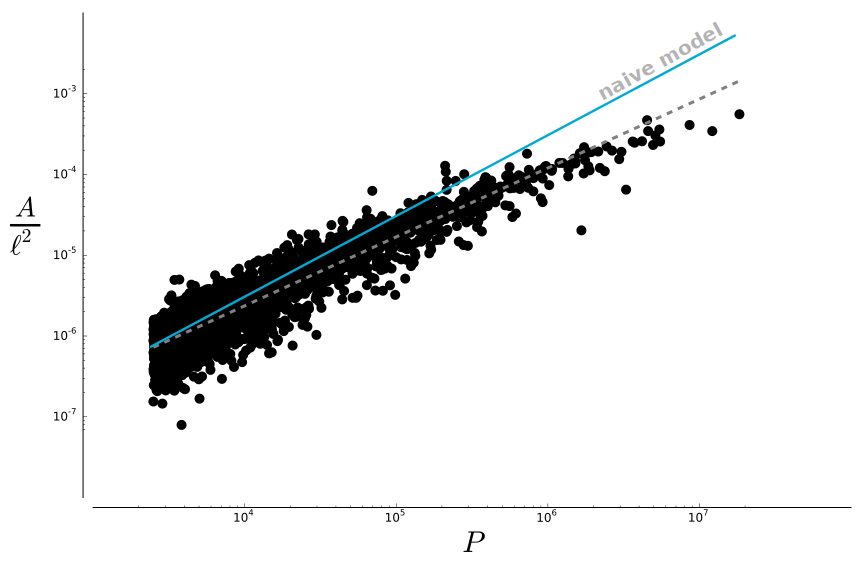
\includegraphics[width=\textwidth]{gfx/chapter-scaling/scaling_area.pdf}
    \caption{{\bf Spatial footprint.} Scaling of the surface area of US urban areas with population size,
        and what would be expected with a naive model (blue solid line).
    A fit assuming a powerlaw dependence (dashed line) gives an exponent
    $\beta_A = 0.85 \pm 0.01\,(r^2 = 0.93)$.\label{fig:scaling_area}}
\end{figure}



\subsection{Total length of road}
\label{sub:total_length_of_road}

\paragraph{Naive model.} We would now like to estimate the total length $L_N$ of all the roads within a
city. If we consider that the network formed by streets is such that all the
nodes (intersections) are connected to their closest neighbour, the typical
length of a road segment is given by

\begin{equation}
    \ell_R \sim \sqrt{\frac{A}{N}}
\end{equation}

where $N$ is the number of intersections~\cite{Barthelemy:2008}. Previous studies of road networks in
different regions, and over extended time
periods~\cite{Strano:2012,Barthelemy:2013}, have shown that the number of
intersections is proportional to the population size. Therefore, the typical
length of a road segment (between two intersections) varies with the population
size $P$ as

\begin{equation} 
    \ell_R \sim \sqrt{\frac{A}{P}} 
    \label{eq:length_nodes}
\end{equation}

and the total length of the network $L_N \sim P\ell_R$ should then scale as

\begin{equation} 
    \frac{L_N}{\sqrt{A}} \sim \sqrt{P} 
\end{equation}

Using the naive scaling for the dependence of $A$ on population size given
previously in Eq.~\ref{eq:area_naive} we finally get 

\begin{equation} 
    L_N \sim P
\end{equation}

\paragraph{Reality.} Again, the naive argument does not compare well with
reality. We fit the data for US Urban Areas (see
Figure~\ref{fig:scaling_lanemiles}) assuming a powerlaw dependence and find an
exponent

\begin{equation}
    \boxed{\beta_R \sim 0.765 \pm 0.033\;(r^2 = 0.92)}
\end{equation}

Note that the relation between the length and the number of nodes given by
Eq.~\ref{eq:length_nodes}, as well as the relation between number of
intersections and population, have been verified independently in the
literature. The observed discrepancy on the exponent of $L_N$ is therefore
certainly due to the scaling of the surface area.

\begin{figure}
    \centering
    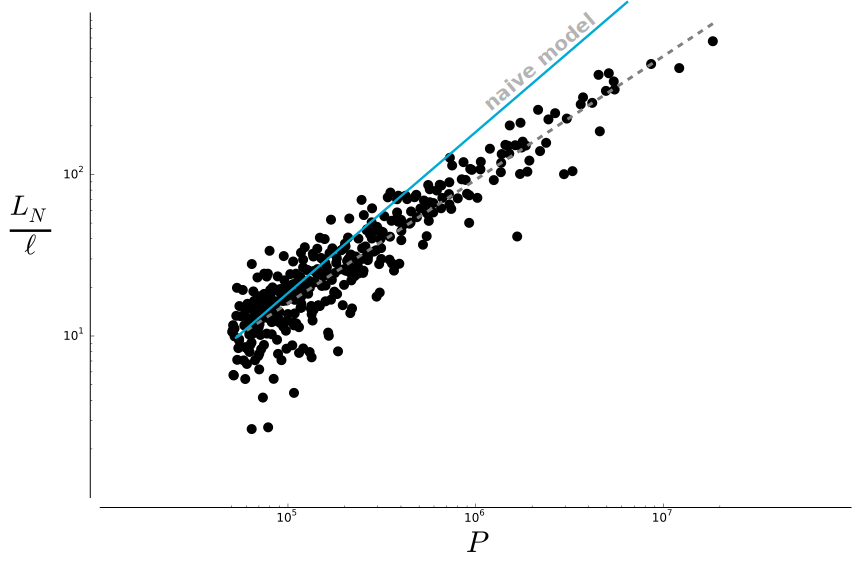
\includegraphics[width=\textwidth]{gfx/chapter-scaling/scaling_lanemiles.pdf}
    \caption{{\bf Length of roads.} Scaling of the total length of roads in US Urban Areas versu the
    total population. A fit assuming a powerlaw dependence (dashed grey line)
gives an exponent $\beta_R \sim 0.765 \pm 0.033$ ($r^2=0.92$). The behaviour is
qualitatively different from what would be expected with a naive model (solid
blue line).\label{fig:scaling_lanemiles}}
\end{figure}



\subsection{Total commuting distance}
\label{sec:total_length_driven}

The total commuting distance $L_{tot}$ is determined by two different
constraints. First the individual constraint: individuals make the decision
about where they are going to live and work; they have their own behaviour and
limitations. However, the individuals' choices are also limited by the city
structure itself, that is by the respective distributions of jobs and residences across the
city.



\subsubsection{Influence of the individual constraint} 

The first constraint on the commuting distance comes from individuals' limitations and
behaviour. We make here the simple assumption that individuals choose their
residence and work place such that their total commuting distance is fixed (or
at least, is smaller than a certain value) and equal on average to $\ell_C$. In that
case, we would simply have

\begin{equation} 
    \frac{L_{tot}}{P} \sim \text{constant} = \ell_c 
    \label{eq:assum}
\end{equation}

(by constant, we mean independent from the population size of the city). As
surprising as it may seem, the data show that $L_{tot}/P$ can indeed be considered
 independent from $P$ (with a value of approximately $23$ miles for
the US, see Figure~\ref{fig:LtotoverP}), in agreement with the individual
constraint assumption (Eq. \ref{eq:assum}). This finding is also in agreement
with the results drawn from census data in Germany by~\cite{Wilkerson:2014}.
This does not mean, of course, that the distance driven is the same for every
city. As one can see on Figure~\ref{fig:LtotoverP}, the fluctuations are quite
important between cities.  

\begin{figure}[!h]
    \includegraphics[width=1.0\textwidth]{gfx/chapter-scaling/figure_2.pdf}
    \caption{{\bf Commuting distance \& individual choice.} Constant daily driven distance per capita. (a) daily total driven
        distance per capita as a function of population for 441 urbanised area
        in the US in 2010. The data shown in the plot are compatible with a
    population-independent behaviour. (b) Histogram of the daily total driven
distance per capita for the same cities. The average daily driven distance is $23$ miles, and the standard deviation $7$ miles.}
\label{fig:LtotoverP} 
\end{figure}



\subsubsection{Influence of the city structure}
\label{sub:influence_of_the_city_structure}

The easiest way to understand the influence of the city constraints is to
consider two limiting cases: the totally centralised
(monocentric) city where everyone goes to work to a single center, and the
totally decentralised city where everyone goes to work to the nearest
location (see Figure~\ref{fig:monocentric_decentralised})~\cite{Samaniego:2008}.\\

\begin{figure}[!h]
    \centering
    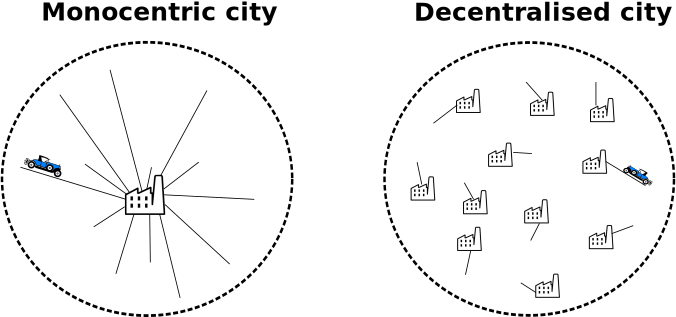
\includegraphics[width=1\textwidth]{gfx/chapter-scaling/monocentric-decentralised.pdf}
    \caption{{\bf Limiting cases.} Representation of the monocentric city (left) and the totally
    decentralised city (right), two extreme models for the shape of mobility
patterns.\label{fig:monocentric_decentralised}}
\end{figure}

\paragraph{Monocentric.} If we first assume that the city is monocentric, individuals are all commuting
to the same center and the typical commuting distance $\ell^m_c$ is controlled
by the typical size of the city of order $\sqrt{A}$, so that

\begin{equation} 
    \frac{L_{tot}^{m}}{\sqrt{A}} \sim P 
\end{equation}

\paragraph{Decentralised.} On the other hand, if we assume that the city is completely decentralised, the
typical commuting distance is of order the nearest neighbour distance
$\sqrt{A}/\sqrt{P}$, and we obtain

\begin{equation} 
    \frac{L_{tot}^{d}}{\sqrt{A}} \sim \sqrt{P} 
\end{equation}

\paragraph{Reality. } The scaling of the total driven distance for Urban Areas
(morphological definition) is shown on
Figure~\ref{fig:scaling_Ltot_norm}, and the exponent sits between the ones of the
monocentric and decentralised cities

\begin{equation*}
    \boxed{\beta_L =  0.595 \pm 0.026\; (r^2 = 0.90)}
\end{equation*}


\begin{figure}
    \centering
    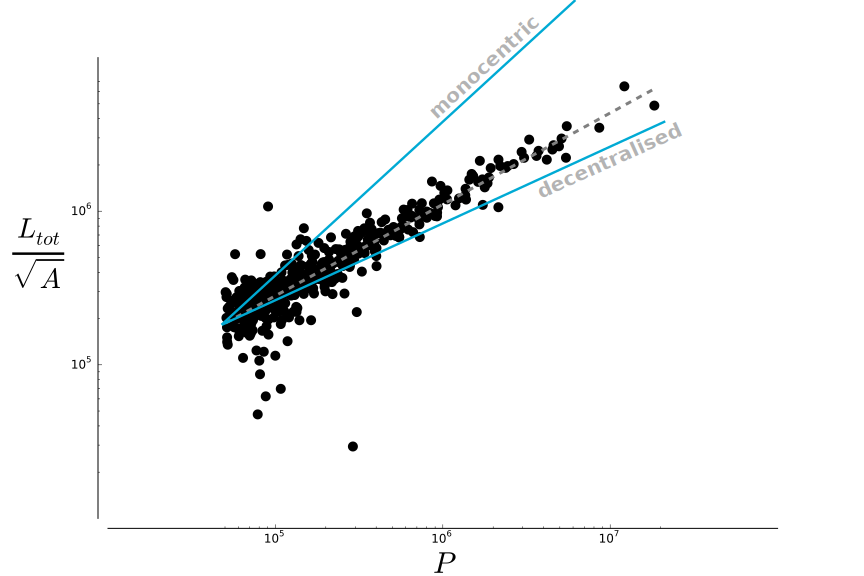
\includegraphics[width=0.9\textwidth]{gfx/chapter-scaling/scaling_commuting_norm.pdf}
    \caption{{\bf Commuting distance \& city structure.} Scaling of the total yearly commuted distance normalised by the
    city's surface area with population size for US Urban Areas. The blue lines
show the behaviours that would be expected for a monocentric and a totally
decentralised city. The dashed line represents the fit assuming a powerlaw
dependence, which yields an exponent $\beta =  0.595 \pm 0.026\, (r^2 =
0.90)$.\label{fig:scaling_Ltot_norm}}
    
\end{figure}

This comes as another evidence -- different from that presented in
Chapter~\ref{chap:monocentric_introduction} -- that cities do not have a
strictly monocentric structure. This result casts some further doubts about the
model by Bettencourt~\cite{Bettencourt:2013} which implicitely assumes that
cities are monocentric.\\

So far, so good. But how can we understand the non-trivial exponent that is observed? This is
where the limiting case are helpful: if the exponent sits between the ones that
would be obtained in a monocentric or decentralised city, surely, cities must
adopt an intermediate structure. 

\begin{figure}[!h]
    \centering
    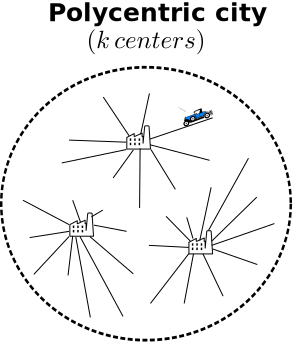
\includegraphics[width=0.4\textwidth]{gfx/chapter-scaling/polycentric.pdf}
    \caption{{\bf Polycentric structure.} City with a polycentric structure, intermediate between the
    monocentric and totally decentralised situations. \label{fig:polycentric}}
\end{figure}

One candidate stands out: the polycentric city (see
Figure~\ref{fig:polycentric}). Let us thus consider a polycentric city with $k$
employment centers. The typical distance commuted by individuals is then given by

\begin{equation}
    \ell_c \sim \sqrt{\frac{A}{k}}
\end{equation}

So that

\begin{equation}
    \frac{L_{tot}}{\sqrt{A}} = \frac{P}{\sqrt{k}}
\end{equation}

Therefore if, as we showed in the previous part,  the number of centers
increases sublinearly with population, we would have a scaling of the form
$L_{tot}/\sqrt{A}\sim P^{\,\beta_L}$ where $\beta_L \in [1/2,1]$. The previous
expression is consistent with that of $A/\lambda^2$ and $L_{tot}/P$ if

\begin{equation} 
    \beta_L = 1-\frac{\beta_A}{2} 
    \label{eq:consis} 
\end{equation}

which is indeed what we observe empirically (up to error bars). We conclude from
this preliminary empirical analysis that, in order to compute the various
exponents, we need to better describe the structure of commuting patterns. In
other words, we need to find a description of cities that goes beyond the naive
monocentric or totally decentralized views, and which accounts for the observed
sub-linear scaling of the surface area $A$.



\begin{table*}[!h]
    \centering
\begin{tabular}{|c|c|c|l|}
\hline
Quantity & Naive exponent &  Measured value\\
\hline
$A $ & $1$ & $0.85\; (r^2=0.93)$\\
\hline
$L_N / \sqrt{A}$ & $0.5$ & $0.42\; (r^2=0.83)$\\
$L_N $ & $1$ & $0.89\;(r^2=0.77)$\\ 
\hline
$L_{tot} / \sqrt{A}$ &  $\left\{0.5,1\right\}$ & $0.60\; (r^2=0.90)$\\
$L_{tot} /P$ &  $1$ & $0.03\; (r^2=0.04)$\\
\hline
\end{tabular}
\caption{{\bf Naive exponents and measured values.} This table displays the value of the exponent governing the behavior with the population $P$ obtained by naive arguments and the value obtained from empirical data. The discrepancies reveal the failure of the naive scaling arguments and the necessity to go further and model mobility patterns.}
\label{table:naive}
\end{table*}



\section{Beyond naive scalings: modeling the mobility patterns}

The previous results, in particular the behaviour of the total commuting length
with population, hint at the necessity to better describe the structure of the
mobility patterns (Table~\ref{table:naive}). This is exactly what the model presented in the previous
chapter does. 

Using the relation that we derived for the number of centers, we will see
how we can understand the values of the exponents presented earlier in this
chapter. We will also see how the model allows us to understand the scaling of
other quantities, namely the total time spent in traffic and the total $CO_2$
emissions due to transportation.

\subsection{Area}

According to the model introduced in Chapter~\ref{chap:monocentric_model}, the number of centers is a function of population and the area

\begin{equation}
    k = F\left(A,P\right)
\end{equation}

and we need an additional equation in order to get a closed system. Here we
focus on the area and its evolution with the population size, which reflects the
growth process of the city. 

In the following, we will investigate two different
approaches. It is worth noting that both approaches give results in qualitative
agreement, showing that some stylized facts ---such as super- or sublinearity---
are very robust.\\ 

\paragraph{Fitting procedure.}

In the absence of knowledge of the processes responsible for urban sprawl, we
can assume that the area behaves as 

\begin{equation}
    A \sim P^{\,a}
    \label{eq:fit}
\end{equation}

where $a$ is the exponent to be determined by fitting data. The empirical
value for the exponent for the US data is $a\simeq 0.85$. Once this exponent is
given we can then compute the various exponent for the quantities of interest.
We get for the number of centers $k$

\begin{equation}
    k \sim P^{\frac{\mu + a/2}{\mu+1}}
\end{equation}

which is sublinear as long as $a<2$, in agreement with the empirical results for
US cities. As we will see, this approach yields the same qualitative behaviours
as those predicted with the method of the next section. In other words, even if
the main mechanism behind urban sprawl is not congestion, the conclusions of
this paper are not affected as long as the area scales \emph{sublinearly} with
population.\\


\paragraph{Coherent growth.}

Let us now assume that the scaling of $A$ with population is determined by the
number of activity centers and the constant commuting length of individuals.
This means that the growth of the area is controlled by the appearance of new
activity centers. 

If we assume that a city is organized around $k$ activity
centers and that the attraction basin of each of these centers are spatially
separated~\cite{Louf:2013_polycentric} (See on Figure~\ref{fig:polycentric}), we then have  $A \sim k\, A_1$ where $A_1$ is the
area of each subcenter's attraction basin. This area $A_1$ is related to the
average individual commuting distance by $\sqrt{A_1} \sim L_{tot} / P$, and we
obtain

\begin{equation}
    A \sim k\,  \left( \frac{L_{tot}}{P} \right)^2 = k\, \ell_c^2
    \label{eq:area_poly}
\end{equation}

This leads to expression for the number of centers

\begin{equation}
    k \sim P^{\frac{2 \mu}{2\mu+1}}
\end{equation}

which is always smaller than $1$, also in agreement with the empirical results
for US cities. We can now also compute the scaling of the surface area

\begin{equation}
    \frac{A}{\ell_c^2} \sim \left( \frac{P}{c} \right)^{\frac{2 \mu}{2\mu+1}}
\end{equation}

We further assume that $L_{tot} / P$ is a fraction of the longest possible
journey $\ell$ individuals can afford, that is to say 

\begin{equation}
    \ell_c \sim \ell
\end{equation}

It is important to note that if $\ell_c$ is independent from $\ell$, the
quantitative predictions of our model would still hold. 

The final expression for the area is then here given by

\begin{equation}
    \frac{A}{\ell^2} \sim \left( \frac{P}{c} \right)^{\,2\,\delta}
    \label{eq:area}
\end{equation}

where $\delta=\frac{\mu}{2\mu+1}$. The exponent $\delta$ is smaller than $1/2$
whatever $\mu\geq 0$, which implies that the surface area of cities increases
\emph{sublinearly} with population. In other words, the density of cities
\emph{increases}  with population. This prediction is verified with data about
land area of urbanized areas in the US (Figure~\ref{fig:scaling_area}). We find
$\beta_A = 0.85 \pm 0.01\;$ which is not too far from the
theoretical value $2\delta_{th} = 0.64 \pm 0.12$, equal to
$\alpha$ in this case.\\

Because the area of a city results from centuries of evolution, we do
not a priori expect our model -- where individual vehicles are assumed to be the
only vector of mobility -- to give a prediction valid for all countries and all
times. Nevertheless, these results give us reasons to believe that the spatial
structure of the journey-to-work commuting might be the dominant factor
in the dependence of land area on population. In the following, we will use the
above numerical value to compute other scaling exponents.


\subsection{Total commuting distance}

Using Eq.~\ref{eq:assum} and Eq.~\ref{eq:area} we are now able to compute $L_{tot}/\sqrt{A}$

\begin{equation}
    \frac{L_{tot}}{\sqrt{A}} = P\; \left(\frac{P}{c}\right)^{-\delta}
    \label{eq:travelled_length}
\end{equation}

We plot $L_{tot} / \sqrt{A}$ for urbanized areas in the US on
Figure~\ref{fig:scaling_Ltot_norm}, and one
can verify in Table~\ref{table:results} that the exponent predicted from the previously measured
value of $\alpha$ agrees well with the exponent measured on the data.


\subsection{Total length of roads}

If we use the previously derived expression for the area $A$, we find

\begin{equation}
    L_N \sim \ell \; \sqrt{P}\; \left(\frac{P}{c}\right)^{\,\delta}
\end{equation}

The quantity $\delta$ is less than $1/2$, which implies that $L_N$ scales
\emph{sublinearly} with the city's population size. In other words, larger
cities need less roads per capita than smaller ones: we recover the fact that
 the agglomeration of people in urban centers involves economies of scale for
infrastructures. 


\subsection{Total delay due to congestion}

\begin{figure}
    \centering
    \includegraphics[width=\textwidth]{gfx/chapter-scaling/scaling_delay.pdf}
    \caption{{\bf Congestion and delay.} Scaling of the total delay due to congestion of US urban areas with
    population size. A fit assuming a powerlaw dependence of the total delay on
population size yields an exponent $\beta_D = 1.270 \pm 0.067\;(r^2=0.97)$.\label{fig:scaling_delay}}
\end{figure}

Unfortunately, the agglomeration of activities in cities does not only generate economies.
Congestion, for instance, is a major diseconomy associated with the
concentration of people in a given area. A simple way to quantify the
impairement caused by traffic congestion is through the total delay it
generates. If we make the first order approximation that the average free-flow
speed $v$ is the same for everyone, the total delay due to congestion is given
--according to our model-- by

\begin{equation} 
    \delta \tau = \frac{1}{v} \sum_{i,j} d_{ij} \left(\frac{T_j}{c} \right)^\mu 
\end{equation}

If we assume that all the centers share the same number of commuters -- a
reasonable assumption within the model presented in
Chapter~\ref{chap:monocentric_model}~\cite{Louf:2013_polycentric} -- we obtain

\begin{equation} 
    \delta \tau \sim \frac{L_{tot}}{v} \left( \frac{P}{k}
\right)^{\mu} 
\end{equation} 

which, using the expressions for $L_{tot}$ and $A$
given in Eq.~\ref{eq:travelled_length} and Eq.~\ref{eq:area} respectively, gives

\begin{equation} 
    \delta \tau \sim \frac{\ell\; P}{v}\;\left(\frac{P}{c}\right)^{\delta} 
\end{equation}

The total commuting time corresponding to the same distance but without
congestion scales as $\tau_0\sim L_{tot}$ and thus less rapidly than the total
delay which scales \emph{super-linearly} with population (even when
polycentricity is taken into account). This means that, for the largest cities,
delays due to congestion actually dominate the time spent in traffic, and that
economical losses \emph{per capita} due to the time lost in congestion --and the
corresponding strain on people's life-- increase with the size of the city. 

The prediction $1+\delta = 1.32$ agrees well with the empirical measure (see
Table~\ref{table:results} and Figure~\ref{fig:scaling_delay})

\begin{equation}
    \boxed{\beta_D = 1.270 \pm 0.067\;(r^2 = 0.97)}
\end{equation}

\subsection{Transport related $CO_2$ emissions}

Another diseconomy associated with congestion is the quantity of $CO_2$ emitted
by cars and the gasoline consumed by motor vehicles. This amount not only
depends on the distance that has been driven, but also on the traffic during the
journey. It indeed turns out that for the same length driven, a car burns more
oil when the traffic is heavy than when the road is clear.  Within our model,
the presence of traffic is seen in the time spent to cover a given distance, and
we write that the quantity of $CO_2$ emitted by a vehicle is proportional to the
total time spent in traffic, leading to

\begin{equation}
    Q_{CO_2}  = q \sum_{i,j} d_{ij} \left[ 1+ \left( \frac{T_j}{c} \right)^\mu \right]
\end{equation}

where $q$ is the average quantity of $CO_2$ produced per unit time. In the
polycentric case with $k=k(P)$ subcenters, the typical trip length
$\overline{d_{ij}}$ is given by $\sqrt{A/k}$ and we obtain

\begin{equation}
    Q_{CO_2} = q\, \ell\, P \left[ 1 + \left(\frac{P}{c}\right)^{\delta} \right]
\end{equation}

The first term in brackets is a constant, and the quantity of $CO_2$ is thus
dominated by congestion effects at large populations

\begin{equation}
    Q_{CO_2} \sim q\; \ell\; P \left(\frac{P}{c}\right)^{\delta}
\end{equation}



and the total daily transport-related $CO_2$ emission per capita thus scales as 

\begin{equation}
    \frac{Q_{CO_2}}{P} \propto  q\ell \left(\frac{P}{c}\right)^{\delta}
\end{equation}

The quantity of $CO_2$ emitted per capita in cities thus increases with the size
of the city, a consequence of congestion. This prediction agrees with the
exponent we measure (Figurere~\ref{fig:scaling_co2}) on data gathered for US and OECD cities (see
Table~\ref{table:results})

\begin{equation}
    \boxed{\beta_C = 1.262 \pm 0.089\;(r^2=0.94)}
\end{equation}

\begin{figure}
    \includegraphics[width=0.9\linewidth]{gfx/chapter-scaling/scaling_co2.pdf}
    \caption{{\bf Congestion and $CO_2$ emissions.} Variation of $CO_2$
emissions due to transport with city size. In blue, excess $CO_2$ (in tons) due
to congestion, as given by the Urban Mobility Report (2010) for 101 metropolitan
areas in the US. In green, we show the estimated $CO_2$
emissions (in tons) due to transports, as given by the OECD for 268 metropolitan
areas in 28 different countries. The dashed yellow lines represent the least-square fit
assuming a power-law dependency with multiplicative noise, which gives
respectively $Q_{CO_2} \sim P^{1.262 \pm 0.089} (r^2=0.94)$ for the US data and
$Q_{CO_2} \sim P^{1.212 \pm 0.098} (r^2=0.83)$ for the OECD data.
\label{fig:scaling_co2}} 
\end{figure}



\section{Discussion}

\subsection{Travel-time budget and congestion}

The total commuting time $T$ can be written as

\begin{equation}
    T = \tau_0 + \delta\,\tau
\end{equation}

where $\tau_0 = L_{tot} / v \sim P$ is the free-flow commuting time and $\delta
\tau \sim P^{1+\delta}$ the excess commuting time computed above. The first
thing we notice when looking at the respective population dependence of both
quantities, is that, in large cities, the total commuting time is dominated by
the time spent in congestion. Indeed, we have

\begin{equation}
    \displaystyle \frac{T}{\delta_\tau} \xrightarrow[\:P \gg 1\:]{} 1
\end{equation}

Which agrees with one's (at least our) experience of driving in large cities.

The second remark is linked to a long-standing belief in the study of urban
systems that individuals possess a constant travel-time
budget~\cite{Zahavi:1974}. We can easily see, however, that this hypothesis is
wrong. Indeed, in the limit of large cities, the individual commuting time is
given by

\begin{equation}
    \frac{\delta_\tau}{P} \sim P^{\,\delta}
\end{equation}

In other words, the \emph{individual commuting time increases with the size of the
city}. Note that not only is this a consequence of the model, but also of the
data analysis (see Figure~\ref{fig:scaling_delay}). The constant travel-time
budget hypothesis is thus refuted. The reason for the discrepancy between
previous measures and our results comes from the fact that these studies
considered averages over large regions, rather than averages at the city
level.

\subsection{Newman \& Kenworthy}

\begin{figure}
    \centering
    \includegraphics[width=\textwidth]{gfx/chapter-scaling/newman_kenworthy.pdf}
    \caption{{\bf Newman \& Kenworthy.} Per capita $CO_2$ emissions versus the population density of cities
    belonging to OECD countries. The cities also present in the Newman \&
    Kenworthy dataset are represented in red. This curve casts serious doubt on
the fact that energy consumption is a simple funtion of
density.\label{fig:newman_kenworthy}}
\end{figure}

The consumption of gasoline is proportional to the emission of $CO_2$ and the time spent driving.
The total daily gasoline consumption is thus given by

\begin{equation} 
    Q_{gas} \sim q\; \ell\; P \left(\frac{P}{c}\right)^{\delta}
\end{equation}

where $q$ is the average quantity of gasoline needed per unit time. From this
expression, we see that the total daily gasoline consumption per capita scales
as

\begin{equation} 
    \frac{Q_{gas}}{P}\sim \ell\, \sqrt{\frac{P}{\rho}} = \ell
\sqrt{A} 
    \label{eq:nk_area}
\end{equation}

and is therefore not a simple function of population density, in contrast with
what was suggested by the seminal paper of Newman and
Kenworthy~\cite{Newman:1989}. We plot on Figure~\ref{fig:newman_kenworthy},  the average individual $CO_2$ emissions (used as a proxy for gasoline
consumption) as a function of the density for OECD cities. The points
corresponding to cities that were in the original study~\cite{Newman:1989} are
highlighted. The relation is a lot less clear than the one presented originally.  

We then plot the same quantity as a function of $\sqrt{A}$, the prediction given
by Eq.~\ref{eq:nk_area}, on Figure~\ref{fig:nk_model}. As one can see, the
prediction is far from perfectly followed. If anything, this figure, combined to
Figure~\ref{fig:newman_kenworthy} show that the debate, in the absence of a
clear-cut conclusion, is not over. At this stage, more data about gasoline
consumption -- preferably for cities belonging to the same system of cities --
is needed to explore this prediction.

\begin{figure}
    \centering
    \includegraphics[width=\textwidth]{gfx/chapter-scaling/nk_model.pdf}
    \caption{{\bf Newman \& Kenworthy revisited.} Per capita $CO_2$ emissions versus $\sqrt{A}$ for cities of
    countries that belong to the OECD. The dashed line represents the obtained
linear fit, as predicted by Eq.~\ref{eq:nk_area} ($r^2=0.55$). The agreement is
poor, which may be due to the fact that cities all belong to different systems
of cities (and thus have a different prefactor).\label{fig:nk_model}}
\end{figure}

\subsection{Monocentric versus polycentric}

Although polycentricity emerges naturally from our model as a result of
congestion, many circumstances can prevent or foster the appearance of new
activity centers in a city. There are many debates as to whether policies should
favour polycentric or monocentric developement of cities. Most of them are
based on ideologies and opinions about how cities should be, very few are based
on a quantitative understanding of the city as a complex system. Although this
only represents a small part of the debate, our model allows to quantify the
effect of polycentricity on the total delay due to congestion.

We can indeed compute the total delay due to congestion in the case of a
monocentric configuration. In this situation, all the population commutes to a
single destination $1$ and we have

\begin{equation}
    \delta \tau_{mono} = \frac{1}{v}\; \sum_i d_{i1} \left(\frac{P}{c} \right)^\mu = L_{tot} \left(\frac{P}{c} \right)^\mu
\end{equation}

It follows, using the expression given above for $L_{tot}$

\begin{equation}
    \delta\tau_{mono} = \frac{\ell}{v}\; P^{1+\mu}
\end{equation}

From the fact that $1+\mu > 1+\frac{\mu}{2\mu+1}$, we indeed find that the total
delay due to congestion is worse for monocentric cities than it is for
polycentric cities with the same population, which agrees with the usual
intuition. More precisely the ratio of delays is given by

\begin{equation}
    \frac{\delta\tau_{mono}}{\delta\tau_{poly}}\sim
    \left(\frac{P}{c}\right)^{\,\beta}
\end{equation}

where the exponent is of order $\beta \approx 0.57\;$. Therefore, even though
diseconomies associated with polycentric cities scale superlinearly with
population, it would be even worse if we did not let cities evolve from the
monocentric situation. The same reasoning applies to the consumption of gasoline and
the $CO_2$ emissions. 

This suggests that, everything else being equal,
polycentricity should be favoured for quality of life and environmental reasons.

\begin{table*}[!h]
\begin{tabular}{|c|c|c|c|}
\hline
Quantity & Theoretical expression & Predicted exponent & Measured value\\
  $\;\;$  & ($\delta=\alpha/\alpha+1$) & & \\ \hline
$L_{tot}$ & $P$ & $1$ & $1.03 \pm 0.03\;(r^2=0.95)$\\ 
$A / \ell^2$ & $\left( \frac{P}{c} \right)^{\,2\,\delta}$ & $2 \delta = 0.78 \pm 0.20$ & $0.853 \pm 0.011\; (r^2=0.93)$\\
$L_N / \ell$ & $\sqrt{P}\; \left(\frac{P}{c}\right)^{\,\delta}$ & $\frac{1}{2} + \delta = 0.89 \pm 0.10 $ & $0.765 \pm 0.033\; (r^2=0.92)$\\
$\delta \tau / \tau$ & $P\; \left( \frac{P}{c} \right)^{\, \delta}$ & $1 +
\delta = 1.39 \pm 0.10$ & $1.270 \pm 0.067\; (r^2=0.97)$\\
$Q_{gas,CO_2}/\ell$  & $P\left( \frac{P}{c}\right)^{\delta}$ & $1+\delta=1.39 \pm 0.10$ & $1.262 \pm 0.089\; (r^2=0.94)$\\
& & & $1.212 \pm 0.098\, (r^2=0.83)$\\
\hline \hline
$L_N / \sqrt{A}$ & $\sqrt{P}$ & $0.5$ & $0.42 \pm 0.02\;(r^2=0.83)$\\
$L_{tot} / \sqrt{A}$ &  $P\;
\left(\frac{P}{c}\right)^{-\delta}$ & $1 - \delta = 0.61 \pm 0.10$ & $0.595 \pm 0.026\; (r^2=0.90)$\\
\hline
\end{tabular}
\caption{{\bf Summary of the scaling exponents.} This table displays the predicted theoretical behavior and
  the empirical observations versus the population size $P$ for
  different quantities: $L_{tot}$ is the daily total driven distance,
  $A$ is the area of the city, $L_{N}$ is the total length of the road
  network, $\delta\tau$ is the daily total delay due to congestion,
  $Q_{gas}$ is the yearly total consumption of gasoline and $Q_{CO_2}$
  is the total $CO_2$ emissions emitted yearly due to
  transportation. In the third column, we show the predicted values of
  the exponent of $P$ using the value of $\alpha$ measured on US
  employment data, and in the fourth column, the value of the
  exponents directly measured on data about US and OECD cities. The
  measured values are in good agreement with the prediction. In
  particular, the exponents for $L_N$ and $\delta \tau$ are consistent
  with our prediction that their difference should be $1/2$.}
\label{table:results}
\end{table*}


\subsection{Outlook}

The superlinear increase of congestion delay with population, and thereby of
gasoline consumption and of $CO_2$ emissions, has terrible consequences on the
economy, the environment, health and well-being. The outlook is nothing short of
grim in our ever-urbanising world. As the proportion of human beings living in
cities dramatically increases -- the UN expects the world population to be $67\%$
urban in 2050 -- wages are likely to \graffito{Estimates are given in the United
Nations' 2011 World Urban Propects.}
increase~\cite{Bettencourt:2007} but not enough to compensate for the negative
effects of congestion. As a result, if the individual car stays the dominant
transportation mode, cities will put more strain on people's life, while acting
as catalysts for the production of $CO_2$ greenhouse gas, which is responsible for an
overall increase of the planet's temperature~\cite{Oreskes:2004}. 

It is currently believed that advantages associated with living in a large city
outweigh the costs. Our results reveal however the existence of very rapidly
growing problems such as congestion and $CO_2$ emissions, which inevitably begs
the question of the sustainability of large cities. It might be time to cut down
considerably the use of individual vehicles, or to consider the possibility of
living in smaller or medium sized cities: the infrastructure costs ($L_N$) may
be larger, but the impact on the environment ($CO_2$ emissions) and on the
well-being of people (delays in congestion) would be beneficial.\\

The most striking fact about the above results is that despite the apparence of
complexity that is conveyed by cities, most of their structure can be explained
by the very simple and universal desire for the best achievable balance between
income and commuting costs. Our model unifies mobility patterns, spatial
structure of cities and allometric scalings in a framework that can be built
upon. 

\chapter{Interpretation and implications of scaling laws}
\label{chap:scaling_implications}

\bigskip


\section{What cities?}
\label{sec:what_cities_}

\cite{Louf:2014_smog} for problem with the $CO_2$\\
\cite{Arcaute:2014} for variation of exponents with city definition.


The success of natural sciences lies in their great emphasis on the role of
quantifiable data and their interplay with models. Data and models are both
necessary for the progress of our understanding: data generate stylized facts
and put constraints on models. Models on the other hand are essential to
comprehend the processes at play and how the system works. If either is missing,
our understanding and explanation of a phenomenon are questionable. This issue
is very general, and affects all scientific domains, including the study of
cities. \\

Until recently, the field of urban economics essentially consisted in untested
laws and theories, unjustified concepts that supersede empirical
evidence~\cite{Bouchaud:2008}. Without empirical validation, it is not clear
what these models teach us about cities. The tide has turned in recent years,
however: the availability of data is increasing in size and specificity, which
has led to the discovery of new stylized facts and opened the door to a new
science of cities~\cite{Batty:2013}. The recent craze for scaling
laws~\cite{Batty:2008,Bettencourt:2007,Pumain:2004}, for instance, has been an
important new step in the study of urban systems.

These laws present themselves as a power-law relationship between socioeconomic
(GDP, number of patents), structural (length of roads, of cables) quantities
$Y$, and the size of the population $P$ of the city:

\begin{equation}
Y = P^{\, \beta}
\end{equation}


where the exponent $\beta$ can be different from $1$. This type of scaling relation is a signature
of various processes governing the phenomenon under study, especially when the exponent
$\beta$ is not what is naively expected~\cite{Barenblatt:2003}. However, as more and more scaling
relationships are being reported in the literature, it becomes less and less clear what we really
learn from these empirical findings. Mechanistic insights about these scalings are usually
nonexistent, often leading to misguided interpretations.\\

\begin{figure}[!h]
	\centering
	\includegraphics[width=\textwidth]{gfx/chapter-scaling/lost_smog.pdf}
	\caption{ {\bf Are larger cities greener or smoggier?} Scaling of transport-related $CO_2$
emissions with the population size for US cities from the same dataset but at different aggregation
levels. In red, the aggregation is done at the level of urban areas and in green for combined statistical
areas. Depending on the definition of the city, the scaling exponents are qualitatively different, leading
to two opposite conclusions. Data on $CO_2$ emissions were obtained from the Vulcan Project (\url{http://
vulcan.project.asu.ed}) (see~\cite{Fragkias:2013,Oliveira:2014}). Data on the population of urban areas and
metropolitan statistical areas were obtained from the Census Bureau (\protect\url{http://www.census.org}). \label{fig}}
\end{figure}

\begin{figure}
    \centering
    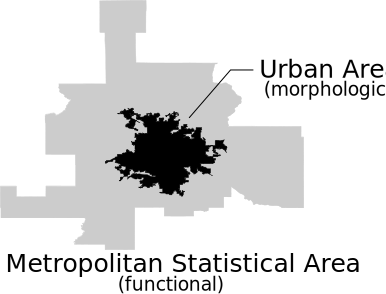
\includegraphics[width=\textwidth]{gfx/chapter-scaling/city_definition.pdf}
    \caption{{\bf City definitions in the US.} The Minneapolis Urban Area (in
    black) is defined by the Census Bureau as contiguous block groups with at
least $1000$ inhabitants per square mile. The Minneapolis-St. Paul Metropolitan
Statistical Area (in grey) is defined as the counties containing the urban area
as well as any adjacent county that have a high degree of integration with the
core, as measured with commuting flows.\label{fig:two_definitions}}
\end{figure}

A striking example of the fallacies which hinder the interpretation and application
of scaling is given by different studies on $CO_2$ emissions due to transportation~\cite{Fragkias:2013,Glaeser:2010,Oliveira:2014,Rybski:2013}. The topic
is particularly timely: pollution peaks occur in large cities worldwide with a seemingly
increasing frequency, and are suspected to be the source of serious health problems~\cite{Bernstein:2004}. Glaeser and Kahn~\cite{Glaeser:2010}, Rybski et al~\cite{Rybski:2013}, Fragkias et al~\cite{Fragkias:2013}, and Oliveira et al~\cite{Oliveira:2014} are interested in how $CO_2$ emissions scale with the population size
of cities. The question they ask is simple: Are larger cities greener---in the sense that there
are fewer emissions per capita for larger cities---or smoggier? Surprisingly, these different
studies reach contradictory conclusions. We identify here two main sources of error which
originate in the lack of understanding of the mechanisms governing the phenomenon.

The first error concerns the estimation of the quantity $Q_{CO_2}$ of $CO_2$ emissions due to
transportation. In the absence of direct measures, Glaeser and Kahn~\cite{Glaeser:2010} have chosen
to use estimations of $Q_{CO_2}$ based on the total distance traveled by commuters. This is in fact
incorrect, and in heavily congested urban areas the relevant quantity is the total time spent
in traffic~\cite{Louf:2013}. Using distance leads to a serious underestimation of
$CO_2$ emissions: the effects of congestion are indeed strongly nonlinear, and the time spent
in traffic jams is not proportional to the traveled distance. As a matter of fact, commuting
distance and time scale differently with population size, and the time spent commuting and
$CO_2$ emissions scale with the same exponent~\cite{Louf:2014}.

The second, subtler, issue lies in the definition of the city itself, and over which
geographical area the quantities $Q_{CO_2}$ and $P$ should be aggregated. There is currently great
confusion in the literature about how cities should be defined, and scientists, let alone the
various statistical agencies in the world, have not yet reached a consensus. This is a crucial
issue as scaling exponents are very sensitive to the definition of the city~\cite{Arcaute:2013}. $CO_2$ emissions are no exception: aggregating over urban areas or metropolitan
statistical areas entails radically different behaviours (see figure~\ref{fig}). For the US, using the
definition of urban areas provided by the Census Bureau (\url{http://www.census.org}), one finds
that $CO_2$ emissions per capita sharply increase with population size, implying that larger
cities are less green. Using the definition of metropolitan statistical areas, also provided by
the Census Bureau, one finds that $CO_2$ emissions per capita decrease slightly with population
size, implying that larger cities are greener.\\



Faced with these two opposite results, what should one conclude? Our point is that, in
the absence of a convincing model that accounts for these differences and how they arise,
nothing. Scaling relationships, and more generally data analysis, have an important role
to play in the rising new science of cities. But, as the previous discussion illustrates, it is
dangerous to interpret empirical results without any mechanistic insight. Conclusions cannot
safely be drawn from data analysis alone.

From a policy point of view, now, what should one do to curb CO2 emissions? Favour
the growth of large urban areas or the repartition of population in less populated cities?
Both can be argued by considering data analysis alone. It should therefore be obvious that,
until they have a satisfactory understanding of the mechanisms responsible for the observed
behaviours, scientists should refrain from giving policy advice that might have unforeseen,
disastrous consequences. If they choose to do so anyway, policy makers should be wary
about what is, at best, a shot in the dark

\section{Scaling and system of cities}
\label{sec:scaling_and_system_of_cities}

We briefly mentionned in the introduction that allometric scaling relationships
could only be obtained when considering cities belonging to the same system of
cities. Indeed, if we mix on the same plot cities from two different countries,
say North-American cities with African cities, it is very likely that we would
obtain very different results. Based on this observation, several questions
arise: First, how does the $Y$ quantity at the level of a country (system)
depend on the properties of its system of cities? How can we understand the
quantity $Y_0$, and how can we sensibly normalise the scaling curves of
different systems of cities to compare their respective trends?

\section{Proviso}
\label{sec:poviso}

Scaling laws are useful tool to probe the system city, but they are not
everything. They provide an extraordinarily easy way to explore the properties
of urban systems: the amount of data required is minimal, the treatment
trivial. However, while it may be useful to declutter the investigation field
and help clear a couple of paths, and help establish a large-scale understanding
of the system, this is done at the expense of an extensive coverage of the
underlying phenomena. Scalings can be seen as a gateway to the study of cities,
but they cannot be the study itself.

The attentive reader might have noticed that I have attempted to be very careful
in specifying the city definition that was used in the different studies in the

Our results
suggest that diseconomies associated with congestion scale superlinearly with
population size, implying that --despite polycentrism-- cities whose
transportation infrastructure rely heavily on traffic sensitive modes are
unsustainable.
iterature, or that I have used myself.

%------------------------------------------------




\ctparttext{Segregation is a notion that is difficult to define, hence the
extensive literature concerning segregation in the literature. In this part, we
propose to measure segregation as a deviation to the unsegregated city. We thus
provide a strong theoretical basis for the location coefficient. We further
derive a measure of attraction of the different categories, that allows us to
define unambiguously classes for the original categories. We study the
properties of neighbourhoods of different classes. We revisit the poor
center/rich suburb distinction. Finally, we propose a new measure of segregation
that takes space into account.} 

\part{Segregation}
\label{part:segregation}

\chapter{What segregation is not}
\label{chap:segregation_introduction}

\begin{flushright}{\slshape    
The limits of my language\\
Mean the limits of my world.} \\ \medskip
--- Ludwig Wittgenstein~\cite{Wittgenstein:1998}
\end{flushright}


\bigskip


% Defining average and variance
\newcommand{\E}{\mathrm{E}}
\newcommand{\Var}{\mathrm{Var}}

\section{Studying segregation}
\label{sec:studying_segregation}


We cannot judge the spatial repartition of people. There is no criterion of
`good' or `bad' for the way people arrange themselves, no moral values attached
to any spatial pattern. It is the \emph{processes} that lead to such patterns,
the intentions behind people's decisions that make segregation condemnable. It
is the \emph{consequences} of segregation that may make undesirable, something
worth fighting against.\\

% consequences
% need for a local information
As a matter of fact, social residential segregation has terrible consequences.
As shown in~\cite{Massey:1993}, residential segregation is the cause of major
economic disadvantages that affect the least affluent segments of the
population, through the isolation from social networks, or the presence of poor
public service in the least affluence zones. Worse, it has been shown that
increased levels of segregation in urban areas is associated with a higher
mortality burden~\cite{Lobmayer:2002}. For all these reasons, there is a
somewhat urgent need to measure the extent of segregation, especially its local
component, and understand the underlying mechanisms.\\

Most authors systematically design a single index of segregation for
territories that can be very large, up to thousands of square
kilometers~\cite{Apparicio:2000}. In order to mitigate segregation, a more
local, spatial information is however needed: local authorities need to locate
where the poorest and richest concentrate if they want to design efficient
policies to curb, or compensate for, the existing segregation. In other words,
we need to provide a clear {\it spatial} information on the pattern of
segregation. We need to identify the areas where levels of segregation are high.

Besides, if we want to design policy or incentives to reduce socio-spatial
stratification and its consequences, we need to understand the processes at
play. We need to understand why segregation patterns exist, and why they
persist. Without mechanistic insights, attempts at regulating segregation may
have unforeseen, possibly damaging consequences.  The processes behind
segregation are however unclear. Schelling's cellular automata
model~\cite{Schelling:1971}, although intellectually stimulating, is very
limited in terms of predictions. More sophisticated models appeared
recently~\cite{Brueckner:1999,Glaeser:2008,Gauvin:2013}, yet the link with the
empirical reality is too thin, and processes are yet to be validated.  In fact,
we believe that the lack of appropriate model is likely due to the lack of
identification of a clear structure, or clear behaviours in the data. The
absence of characterisation of the processes at play in fact stresses the urgent
need to properly characterise the spatial patterns of segregation, and the
dynamics of households (how they move, how their characteristics evolve over
time) and neighbourhoods (how their population changes).\\

In the following, we will therefore focus on the empirical characterisation of
the patterns of segregation. To do so, however, we need to define what we mean
when we talk about residential segregation.

\section{Think first, measure later}
\label{sec:introduction}

% the curse of familiarity 
As stated many times, and at different periods in the sociology
literature~\cite{Duncan:1955m,James:1982,Massey:1988,Reardon:2002}, the study of
segregation is cursed by its intuitive appeal. Pretty much everyone has heard of
segregation, and has an opinion about it. This familiarity with the concept
favours what Duncan and Duncan~\cite{Duncan:1955m} called `naive operationalism':
the tendency to force a sociological interpretation on measures that are at odds
with the conceptual understanding of segregation. In their own words

\begin{quote}
    [Segregation] is a concept rich in theoretical suggestiveness and of
    unquestionable heuristic value. Clearly we would not wish to sacrifice the
    capital of theoretization and observation already invested in the concept.
    Yet this is what is involved in the solution offered by naive
    operationalism, in more or less arbitrary matching some convenient numerical
    procedure with the verbal concept of segregation... (Duncan and Duncan,
    1955~\cite{Duncan:1955m})
\end{quote}

For all its intuitive appeal, segregation is however an intricate, compound
notion whose complexity only reveals itself through careful study. However
tempting it is to start writing measures of segregation that seem `reasonable',
it is necessary to stop and think about the meaning of the notion first. We need to
\emph{think} segregation to be able to provide \emph{useful} measures of
segregation.


\section{The dimensions of segregation}
\label{sec:the_dimensions_of_segregation}

Segregation has been extensively studied in the Sociology and Geography
literature. The most important conceptual heritage of this literature is the
distinction between residential segregation's different dimensions.
Massey~\cite{Massey:1988} first proposed a list of $5$ dimensions (and related
existing measures), which was recently reduced to $4$ by
Reardon~\cite{Reardon:2004}. 

\begin{description}
    \item[Evenness] (and clustering in the continuous
        limit, as shown by Reardon~\cite{Reardon:2004}) is the extent to which
        populations are evenly spread in the metropolitan area.
        Measures of evenness are affected by the fact that
        individuals are not spread uniformly across space in urban areas,
        disregarding of their respective category;

    \item[Exposure] is the extent to which different
        populations share the same residential area. This presupposes defining
        what is meant by `residential area';

    \item[Concentration] is the extent to which populations concentrate in their
        residential area;

    \item[Centralisation] is the extent to which populations concentrate in the
        center of the city. However, we have seen in
        Chapter~\ref{chap:monocentric_introduction} that the notion of center
        was meaningless in large, polycentric urban areas;
\end{description}

We will discuss in details the shortcoming of the measures currently proposed
for each of these dimensions in Chapter~\ref{chap:patterns_segregation}.


\section{The unsegregated city}
\label{sec:null_model_the_unsegregated_city}

The fundamental issue with the picture given by these 4 dimensions lies in the
lack of a general theoretical framework in which all existing measures can be
interpreted.  Instead, we have a patchwork of seemingly unrelated measures that
are labelled with either of the aforementioned dimensions. Although segregation
can indeed manifests itself in different ways, it is relatively straightforward
to define what is \emph{not} segregation: a spatial distribution of different
categories that is undistinguishable from a uniform random
situation~\cite{Jahn:1947}. Therefore, we can simply define segregation as the
following

\begin{quote}
Segregation is any pattern in the spatial distribution of populations that significantly 
deviates from a random distribution. 
\end{quote} 

Our definition is perfectly agnostic with regards of the other features of the
density pattern. It is also not concerned with the overall inequality levels.\\


In the context of residential segregation in urban areas, a natural null model
is therefore the \emph{unsegregated city}. Within the framework of this model,
all households are distributed at random in the city with the further
constraints that

\begin{itemize}
    \item The total number $N_\alpha$ of people belonging to a category
	    $\alpha$ is fixed and equal to that found in the data;
    \item The total number $n(t)$ of households living in the areal unit $t$ is
	    fixed and equal to that found in the data.
\end{itemize}

which also fixes the total number of individuals $N$ in the city. The problem of
finding the numbers $\left( n_\alpha(1), \dots, n_\alpha(T) \right)$ of
individuals belonging to a certain category $\alpha$ in the $T$ areal units of
an unsegregated city is reminiscent of the traditionnal occupancy problem in
combinatorics~\cite{Feller:1950}. Their distribution is given by the multinomial
distribution $f \left( n_\alpha(1), \dots, n_\alpha(T) \right)$, and the number
of people of category $\alpha$ in the areal unit $t$ by a binomial distribution.
Therefore, in an unsegregated city, we have

\begin{align}
    \begin{split}
	\E \left[ n_\alpha(t) \right] &= N_\alpha\,\frac{n(t)}{N} \\
	\Var \left[ n_\alpha(t) \right] &= N_\alpha\,\frac{n(t)}{N} \left( 1 - \frac{n(t)}{N}  \right) 
    \end{split}
\end{align}

where $N$ is the total number of households in the city. In metropolitan areas
$N_\alpha$ is larged compared to $1$, and the distribution of the $n_\alpha(t)$
can be approximated by a Gaussian with the same mean and variance.

The different dimensions of~\cite{Massey:1988,Reardon:2004} correspond then to
particular aspects of how a multi-dimensional pattern can deviate from its
randomized counterpart. The measures we propose here are all rooted in this
general definition of segregation.

Most studies exploring the question of spatial segregation define measures
before comparing their value for different cities. Knowing that two quantities
are different is however not enough: we also have to know whether this
difference is {\em significant}. In order to assess the significance of a
result, we have to compare it to what is obtained for a reasonable null model.
As we will see in Chapter~\ref{chap:patterns_segregation}, the 
`unsegregated city model allows us to assess whether a given pattern is
the result of a segregation process or not.\\

\bigskip

In this chapter, we have discussed some of the improvements that could be
brought to the existing measures in the literature. In particular, we have
emphasized the need for a \emph{local} knowledge of the patterns of segregation.
We have also laid the theoretical foundation upon which we are going to design
new segregation measures.
In Chapter~\ref{chap:patterns_segregation}, we start from the above-defined null
model to propose a way to quantify the presence of various categories in areas
of the city, identify and delineate neighbourhoods, measure the interactions
between the categories and propose measures that fit in the $4$ dimensions
framework.

% !TEX root = ../thesis-example.tex
%
\chapter{Patterns of segregation}
\label{chap:patterns_segregation}

\begin{flushright}{\slshape    
To understand is to perceive patterns.} \\ \medskip
--- Isaiah Berlin~\cite{Berlin:2013}
\end{flushright}


\bigskip


\section{Introduction}
\label{sec:introduction}

\subsection{Shortcomings in the current empirical picture}
\label{sub:shortcomings_in_the_current_empirical_picture}

There are many different ways in which a spatial pattern can deviate from its
randomised counterpart, and at least as many different measures one could
perform. In this chapter, we will try to quantify these patterns in a way that
may allow us to \emph{understand} the phenomenon of segregation.\\

Of course, segregation has been extensively studied in the literature. However,
we identify several difficulties in the current empirical picture.

First, some issues are tied to the existence of several categories in the
underlying data. Historically, measurements of racial segregation were limited
to measures between $2$ population groups. However, most measures generalise
poorly to a situation with many groups, and the others do not necessarily have a
clear interpretation~\cite{Reardon:2002}. Worse, in the case of groups based on
a continuum (such as income), the thresholds chosen to define classes are
usually arbitrary~\cite{Jargowsky:1996}. We propose to solve this issue by
defining classes in a unambiguous and non-arbitrary way through their pattern of
spatial interaction. Applied to the distribution of income categories in US
cities, we find $3$ emergent categories, which are naturally intepreted as the
lower-, middle- and higher-income classes.

Second, most authors systematically design a single index of segregation for
territories that can be very large, up to thousands of square
kilometers~\cite{Apparicio:2000}. In order to mitigate segregation, a more
local, spatial information is however needed: local authorities need to locate
where the poorest and richest concentrate if they want to design efficient
policies to curb, or compensate for, the existing segregation. Furthermore, 
a local description of the repartition of the different categories is the first
step towards the exploration of the mechanisms responsible for segregation: it
is necessary to gather hints (as well as empirical regularities) that are
essential to build a reasonable model. 
In other words, we need to provide a clear {\it spatial} information on the
pattern of segregation.\\



The lack of clear spatial characterization of the distribution of individuals is
not tied to the problem of segregation in particular, but pertains to the field
of spatial statistics~\cite{Ripley:1981}. Many studies avoided this spatial
problem by considering cities as monocentric and circular, and rely on either an
arbitrary definition of the city center boundaries, or on indices computed as a
function to the distance to the center (whatever this center may be, see
Part~\ref{part:polycentricity}). However, most if
not all cities are anistropic, and the large ones, polycentric
(see Chapter~\ref{chap:monocentric_introduction}), casting some doubt about
the application of the monocentric city picture. Many empirical studies and
models in economics aim to explain the difference between central cities and
suburbs \cite{Glaeser:2008, Brueckner:1999}. Yet, the sole stylized fact upon
which they rely -- city centers tend are allegedly poorer than suburbs (in the US) --
lacks a solid empirical basis.\\

In the following, we propose to answer the following questions

\begin{itemize}
    \item How can we quantify the presence of the different categories in areal
        units? Can we say whether they are overrepresented or normally
        represented? How can we define neighbourhoods?
    \item Can we quantify interactions between the different categories?
    \item Can we define meaningful classes from the original data?
    \item Do classes tend to leave in geographically coherent areas, or are they
        scattered across the city?
    \item Is there a difference between the city center and the suburbs? How
        can we quantify this adequately?
\end{itemize}

\subsection{Notations}
\label{sub:notations}

In the following, we will illustrate our measures using data from the $2000$ US
Census on the income of households per Census blockgroup. Data present
themselves as a number of households per blockgroup, sorted in different income
categories. There are $N$ individuals and  $T$ tracts in the considered
geographical area, and we note $N_\alpha$ the number of individuals belonging to
the category $\alpha$.  Finally, we write $n(t)$ the total number of individuals
living in the tract $t$, and $n_\alpha(t)$ the total number of individuals who
belong to category $\alpha$ living in the tract $t$.



\section{Presence of categories}
\label{sec:presence_of_categories}

In order to quantify segregation, we first need to measure the extent to which
categories are spread unevenly across space. Therefore, we start our analysis
with a discussion on how to quantify the presence of a category in areal units.
Several indicators exist, and one needs to be aware of their meaning, their
qualities and their shortcomings. 


\subsection{Concentration index}
\label{sub:concentration}

The concentration index measures the proportion of individuals from category $\alpha$
in the areal unit $t$. 

\begin{equation}
    c(t) = \frac{n_\alpha(t)}{N_\alpha}
    \label{eq:concentration}
\end{equation}

The concentration is composition-invariant: it
does not depend on the relative proportion of category $\alpha$ in the
geographical zone as a whole. 

Nevertheless, its value strongly depends on the total population of the areal
unit we are studying: more populated areal units mechanically entail higher
values of concentration. Segregation measures based on the concentration
(such as the dissimilarity index) will therefore be dominated by the values in
highly populated areal units. This also makes values of concentration difficult
to intepret: we don't know whether large (repectively low) values of
concentration are the result of a large (respective low) population, or of a
local concentration of individuals in the area. 


\subsection{Proportion index}
\label{sub:proportion}

Sometimes, we would prefer to know the proportion of individuals of a given
category in a unit. In our notations, the proportion index is simply defined as 

\begin{equation}
    p(t) = \frac{n_\alpha(t)}{n(t)}
\end{equation}

Although the values of the proportion index are easier to interpret (``x\% of the
individuals living in this areal unit belong to such category''), they are
not a good indicator of segregation. 

Indeed, they strongly depend on the relative proportion of individuals of the
category in the geographical area being studied. For instance, in a city where
$90\%$ of the individuals belong to category $A$, the proportion of people
belonging to category $A$ is very likely to be high in all areal units in the city.
The measure of proportion is therefore strongly tied to the overall inequality
levels.


\subsection{An unbiaised measure: representation}
\label{sub:an_unbiaised_measure_the_representation}

\subsubsection{Definition}
\label{ssub:definition}

The representation solves the problems linked to both measures of concentration
and proportion. The idea behind the measure of representation is that
segregation is, as we argued in Chapter~\ref{chap:segregation_introduction}, a
departure from the situation where households would be spatially distributed
at random. The properties of such a `random', unsegregated city are well known,
and the distribution of categories in each areal unit is given by a binomial
distribution. The representation is
thus defined as the number $n_\alpha(t)$ divided by its expected value in an
unsegregated city, $N_\alpha\,\frac{n(t)}{N}$

\begin{equation}
    r_\alpha(t) = \frac{n_\alpha(t)/n(t)}{N_\alpha/N}
    \label{eq:representation}
\end{equation}

Another way to understand the representation is to compare it to the
above-defined concentration and proportion. We can indeed write

\begin{equation}
    r_\alpha(t) = \frac{c(t)}{n(t) / N} = \frac{p(t)}{N_\alpha/N}
\end{equation}

The representation can thus be interpreted as the concentration
normalised by the local population concentration, or the proportion renormalised
by the proportion of the category at the city level, thereby addressing the
aforementioned shortcomings.\\


\subsubsection{Measuring significant deviations}
\label{ssub:measuring_significant_deviations}


The representation $r_\alpha(t)$ takes values between $0$ (when no
individuals from the category $\alpha$ are present in $t$) and
$\frac{N}{N_\alpha}$ (when all individuals in $t$ belong to the category
$\alpha$). In a city where individuals are distributed uniformly
(see Chapter~\ref{chap:segregation_introduction}), $r_\alpha(t) = 1$ in every
tract $t$.\\


In an unsegregated situation, the values of the representation are likely to be
close to $1$, but not necessarily strictly equal to $1$. There is indeed a
non-zero probability for any distribution to be obtained by chance. It is
therefore not obvious whether a given value of representation could have been
obtained in the unsegregated configuration. However, to quantify segregation, we
need to know how \emph{likely} it is that the present pattern is not the result
of a random repartition of individuals.  In other words, we need to know
whether areal units depart \emph{significantly} from the unsegregated situation. 

The distribution of individuals in a tract $t$ in the unsegregated city follows
a binomial distribution. We can therefore easily compute how likely it is that
the representation $r_\alpha(t)$ we measure has been obtained by chance. To do
that, we first compute the variance of the representation in the unsegregated
configuration:

\begin{equation}
    \mathrm{Var}\left[r_\alpha(t)\right] = \sigma_\alpha(t)^2 = \frac{1}{N_\alpha} \left[\frac{N}{n(t)} - 1\right]
\end{equation}

We say that the representation departs \emph{significantly} from the
unsegregated configuration if we can be sure with $99\%$ confidence that the
pattern has not been obtained at random. It follows that

\begin{itemize}
    \item $\alpha$ is {\bf overrepresented} in $t$ iff $r_\alpha(t) > 1 +
  2.57\;\sigma_\alpha(t)$
    \item $\alpha$ is {\bf underrepresented} in $t$ iff $r_\alpha(t) < 1 +
  2.57\;\sigma_\alpha(t)$
\end{itemize}

Note that the expression of the representation (Eq. \ref{eq:representation}) is very
similar to the formula used in economics to compute comparative
advantages~\cite{Balassa:1965}, or to the localisation quotient used in various
contexts~\cite{Apparicio:2000, Schwabe:2011}. To our knowledge, however, this
formula has never been justified by a null model in the context of residential
location. 

The representation allows to assess the significance of the deviation
of population distributions from the unsegregated city. As we will show below,
it is also the building block for measuring the level of repulsion or attraction
between populations -- allowing us to uncover the different classes -- and to
identify the neighbourhoods where the different categories concentrate. 

Last, but not least, the representation defined here does not depend on the
class structure at the city scale, but only on the spatial repartition of
individuals belonging to each class. This is essential to be able to compare
different cities where the group compositions -- or inequality -- might differ.
Inequality and segregation are indeed two separate concepts, and the way they
are measured should be distinct from one another. In that sense, the
representation is preferable to the measures of concentration or representation
as a basis to quantify segregation.


\section{Measuring the attraction and repulsion of categories}
\label{sec:measuring_the_attraction_and_repulsion_of_categories}

\subsection{Exposure}
\label{sub:exposure}

If we want to uncover the mechanisms underlying segregated patterns, it is
important to measure and understand the interactions between categories.
However, existing measures do not allow to quantify to which extent different populations
attract or repel one another. What we mean here by interaction is the
co-presence of the different categories in the same areal units, thus potential
interactions. This is the best one can do in the absence of data on the actual
interactions between individuals.

The measure we define is inspired by the M-value first introduced by Marcon \&
Puech in the economics literature~\cite{Marcon:2009} and used as a measure of
interaction in \cite{Jensen:2006}.  These authors were interested in measuring
the geographic concentration of different types of industries. While previous
measures (such as Ripley's K-value) allow to identify departures from a random
(Poisson) distribution, the M-value's interest resides in the possibility to
evaluate different industries' tendency to co-locate.\\

The idea, in the context of segregation, is simple. We consider two categories
$\alpha$ and $\beta$ and we would like to measure to which extent they are
co-located in the same areal unit. Essentially, we measure the representation of
the category $\beta$ as witnessed on average by the individuals in category
$\alpha$, and obtain the following quantity $E_{\alpha\beta}$

\begin{equation} 
    E_{\alpha \beta} = \frac{1}{N_\alpha} \sum_{t=1}^{T} n_\alpha(t)\,r_\beta(t) 
\end{equation}

Although it is not obvious with this formulation, this measure is symmetric:
$E_{\alpha \beta} = E_{\beta \alpha}$. Effectively, the E-value is a measure of exposure,
according to the typology of segregation measures found in~\cite{Massey:1988}.
It is however different from the traditional measure of exposure found in the
literature~\cite{Bell:1954}, as it allows to distinguish between the situations
where categories attract, or repel one another.\\

In the case of an unsegregated city, every household in $\alpha$ sees
on average $r_\beta = 1$ and we have $E_{\alpha \beta} = 1$. 
If populations $\alpha$ and $\beta$ {\em attract} one another, that is if they
tend to be overrepresented in the same areal units, every household $\alpha$
sees $r_\beta > 1$ and we have $E_{\alpha \beta} > 1$ at the city scale. 
On the other hand, if they
{\em repel} one another, every household $\alpha$ sees $r_\beta < 1$
and we have $E_{\alpha \beta} <1$ at the city scale. 


\subsection{Extreme values}
\label{sub:extreme_values}

The minimum of the exposure for two classes $\alpha$ and $\beta$ is obtained
when these two categories are never present together in the same areal unit. Then

\begin{equation}
    E_{\alpha\,\beta}^{min} = 0 
\end{equation}

and the theoretical maximum is obtained when the two classes are alone in the system and
otherwise distributed at random

\begin{equation}
    E_{\alpha\,\beta}^{max} = \frac{N^2}{4\,N_\alpha\, N_\beta}
\end{equation}

These extrema are useful when comparing the exposure values for different
categories, and across different cities.



\subsection{Isolation}
\label{sub:isolation}

In the case $\alpha = \beta$, the previous measure represents the
`isolation' defined as

\begin{equation}
    I_\alpha = \frac{1}{N_\alpha}\sum_{t=1}^{t} n_\alpha(t)\,r_\alpha(t)
\end{equation}

and measures to which extent individuals from the same category are
exposed to their kins. In the unsegregated city, where individuals are
indifferent to others when choosing their residence, we have
$I_\alpha^{min}=1$. On the other hand, in the extreme situation where
individuals belonging to the class $\alpha$ live isolated from the
others, the isolation reaches its maximum value

\begin{equation}
    I_\alpha^{max} = \frac{N}{N_\alpha}
\end{equation}

%Of course, in order to discuss the significance of the values of exposure and
%isolation, one needs to compute the variance of the exposure in the unsegregated
%situation defined earlier. The calculations for the variance as well as for the
%extrema are presented in the Supporting Information. [WATCH FOR THIS ONE]

\section{Emergent social classes}
\label{sec:the_emergent_social_classes}

\subsection{Defining classes}
\label{sub:defining_classes}


The study of income segregation must be rooted in a particular definition of categories
(or classes). There is however no consensus in the literature about how to
separate households in different classes according to their income, and studies
generally rely on more or less arbitrary divisions. While in some particular
cases grouping the original categories in pre-defined classes is justified,
most authors do so for mere convenience. However, as some sociologists
have already pointed out~\cite{Emirbayer:1997}, imposing the existence of
absolute, artificial entities is necessarily going to skew our reading of the
data. Entities such as social classes do not have an existence of their own.
Grouping the individuals into arbitrary classes when studying segregation is
thus problematic: it amounts to imposing a class structure on the society before
assessing the existence of this structure (which manifests itself by the
differentiated spatial repartition of individuals with different income,
segregation).
Furthermore, in the absence of recognized standards, different authors will
likely have different definitions of classes, making the comparisons between
different results in the literature difficult.\\

Here, instead of imposing an arbitrary class structure , we let the class
structure emerge from the data themselves. Our starting hypothesis is the
following: if there is such a thing as a social stratification based on income,
it should be reflected in the households' behaviours. The hypothesis is that households belonging to
the same class should tend to live together, while households belonging to
different classes should tend to avoid one another (It is worth noting that this
\emph{horizontal} definition of segregation is not relevant in every context; in
the 19th century Paris for instance, segregation was also vertical, with rich families
living in the lowest floors of buildings while poor individuals did tend to
live in the highest flats). The idea is thus to define
classes based on the way they manifest themselves through the spatial
repartition of the different categories. Of course, spatial proximity does not
necessarily imply social proximity. In particular, Chamboredon showed that in
some big French housing projects, households belonging to different social
classes were artificially brought in close proximity to one another but did not
necessarily interact with one another~\cite{Chamboredon:1970}\graffito{The work of
Chamboredon was kindly brought to my attention by Yann Renisio.}. We thus assume
here that the social class of housing tenants is not determined in a top-down
fashion, so that the spatial repartition of different income classes reflects
the nature of the interaction between these classes. 


\subsection{Income classes in the US}
\label{sub:income_classes_in_the_u_s_}

We choose as a starting point the finest income subdivision given by the Census
Bureau ($16$ subdivisions) and compute the $16 \times 16$ matrix of $E_{\alpha
\beta}$ values for all cities. We then perform a hierarchical clustering on this
matrix, successively aggregating the subdivisions with the highest $E_{\alpha
\beta}$ values. We stop the aggregation process when the only classes left are
indifferent ($E_{\alpha \beta} = 1$ with $99\%$ confidence) or
repel one another ($E_{\alpha \beta} < 1$ with $99\%$
confidence)~\cite{Louf:2015}. We obtain the dendrogram presented on
Figure~\ref{fig:classes_alluvial}.

\begin{figure}
    \includegraphics[width=\textwidth]{./gfx/chapter-segregation/figure1.pdf}
    \caption{{\bf Emergent classes.} (Left) Alluvial diagram showing the successive aggregations
      of income categories in the clustering process, and
      the value of the exposure at which the aggregation took
      place. The aggregation stops when there is no pair of category
      for which $E>1$, that is when all classes are at best
      indifferent to one another. One can see on this diagram that
      the highest income categories attract one another more (higher values of
      $E_{\alpha \beta}$) than the lowest income categories. (Right) The classes that emerge from our
      analysis, and their respective exposure and isolation values. The lower
      and higher income classes repel one another, while the middle
      income class is indifferent to either other classes.  The
      higher-income class is slightly more coherent than the lower-income,
      which is more coherent than the middle-income class, as
      reflected by the isolation coefficient $I$.}
\label{fig:classes_alluvial}
\end{figure}

Strikingly, the outcome of this method is the emergence of 3 distinct classes:
the higher-income ($47\%$ of the US population) and the lower-income ($42\%$ of the US population) classes
 -- which repel one another strongly while being
respectively very coherent -- and a somewhat meagre middle-income class ($11\%$
of the population) that is relatively indifferent to the other classes. This
result implies that there is some truth in the conventional way of dividing
populations into $3$ income classes, and that what we casually perceive as the
social stratification in our cities actually emerges from the spatial
interaction of people. Surprisingly, however, the middle-income class as
obtained here represents a significantly smaller part of the population than
other definitions.

Our method has several advantages over a casual, arbitrary definition: it only
depends on single tunable parameter, the size of the confidence interval.
Although, once an agreement has been reached, the class structure does not
depend on who is performing the analysis. Its origins are tractable, and can be argued on a
quantitative basis. Because it is quantitative, it allows comparison of the
stratification between different points in time, or between different countries. It
can also be compared to other class divisions that would be obtained using a
different medium for interaction, for instance mobile phone
communications~\cite{Eagle:2010}. 

In the following, we will systematically use the classes thus obtained.



\section{Larger cities are richer}
\label{sec:inter_urban}

At the scale of an entire country, segregation can manifest itself in the
unequal representation of the income classes in different urban areas.
We plot on Figure~\ref{fig:inter-urban} the ratio $
N_\alpha^{>}(H)/N^{>}(H)$ where $N^{>}(H)$ is the number of cities of
population greater than $H$, and $N_\alpha^{>}(H)$ the number of cities of
population greater than $H$ for which the class $\alpha$ is overrepresented.

\begin{figure}[!h]
    \centering
    \includegraphics[width=0.7\textwidth]{./gfx/chapter-segregation/gini_income.pdf}
    \includegraphics[width=0.7\textwidth]{gfx/chapter-segregation/figure3.pdf}
    \caption{{\bf Larger cities are richer.} (Top) Gini coefficient of the income distribution of the $280$ MSA in
    $2000$ versus the number of households in the city. As one can see, there is
    no clear trend. (Bottom) Proportion of cities in which the different classes are
    overrepresented, as a function of the total population of the city. One can
    clearly see that as cities get larger rich people will
    be overrepresented and poor people underrepresented (compared to national
    levels). \label{fig:inter-urban}}
\end{figure}

A decreasing curve indicates that the category $\alpha$ tends to be
underrepresented in larger urban areas, while an increasing curve shows that the
category $\alpha$ tends to be overrepresented in larger urban areas.  The
representation is measured with respect to the total population at the US level.

There is a clear differentiation between cities: among the $276$ MSA in our
dataset, no city exhibits a number of households per class 
that is representative of the US as a whole. Furthermore, the number of cities
where higher-income households are overrepresented increases with the size of
the cities, while the inverse trend is true for lower-income
households. Therefore, larger cities are not richer in the sense that rich
households tend to be overrepresented in large cities, and underrepresented in
small ones.

Surprisingly, this effect is not visible using the Gini coefficient (see
Figure~\ref{fig:inter-urban}). This hints at the limitations of the Gini index
to compare income inequalities across an entire country.


\section{Delineating neighbourhoods}
\label{sec:neighbourhoods}

\subsection{Defining neighbourhoods}
\label{sub:defining_neighbourhoods}

\begin{figure}
    \centering
    \includegraphics[width=0.7\textwidth]{./gfx/chapter-segregation/figure2.png}
    \caption{{\bf Neighbourhoods.} The neighbourhoods in Atlanta for the three different
      income category. In black, the tracts where the corresponding
      class is overrepresented, in white where it is
      underrepresented and in grey where its value is
      indistinguishable from the random distribution. All
      MSA defined for the $2000$ Census exhibit a total exclusion between
      lower-income and higher-income
      neighbourhoods: the pictures for lower- and higher-income classes are the
      perfect negative of one another. In contrast, middle-income households
      are scattered across the city.}
\label{fig:atlanta_neighbourhoods}
\end{figure}

Now that we can identify the areal units where classes are overrepresented, how
can we delineate neighbourhoods?

Considering a category $\alpha$,  we first look for the areal units where the
category is overrepresented. We then consider that two areal units in this set
are part of the same neighbourhood if they are contiguous. Of course, this
approach has limitations (some remarks that sprung in the discussion on the different methods to find
activity centers in Chapter~\ref{chap:monocentric_introduction} are relevant in
this context too), but it gives us a reasonable definition of neighbourhoods to
work with.
Let us now focus on the properties of these neighbourhoods.

\subsection{Clustering}
\label{sub:clustering}

Intra-tract measures such as the exposure are not enough to quantify
segregation. Indeed, areal units where a given class is overrepresented can
arrange themselves in different ways, without the intra-tract measures of
segregation being affected~\cite{White:1983}. In order to illustrate this, we
consider the schematic cases represented on Figure~\ref{fig:checkerboard}, and
assume that  they are obtained by reshuffling the various squares around.
Obviously, the checkerboard on the left depicts a very different segregation
situation from the divided situation on the right while intra-tract measures
would give identical results.\\

\begin{figure}[!h]
    \centering
    
\includegraphics[width=0.7\textwidth]{./gfx/chapter-segregation/figure5.pdf}
    \caption{{\bf Spatial considerations.} Three situations that are identical for intra-areal unit measures,
        but that represent different segregation levels. (Left) The checkerboard
        city popularised by White~\cite{White:1983}, corresponding to a
        clustering value (defined in Eq.~\ref{eq:clustering}) of $C=0$ for the black squares. (Middle) An
        intermediate situation between the checkerboard and the divided city,
        corresponding to $C \approx 0.86$.(Right) The divided city, corresponding to
        $C=1$. \label{fig:checkerboard}} 
\end{figure}


A way to distinguish between different spatial arrangements is then to measure
how clustered the overrepresented areal units are. We first aggregate adjacent
overrepresented areal units (for a given class) leading to consistent
neighbourhoods. The ratio of the number $N_n$ of neighborhoods (clusters) to the
total number $N_o$ of overrepresented areal units measures the level of
clustering and in 

\begin{equation} 
    C = \frac{N_{o}-N_{n}}{N_{o}-1}
    \label{eq:clustering}
\end{equation}


such that this quantity is $C = 0$ in a checkerboard-like situation, and $C = 1$
when all areal units form a unique neighbourhood. We show on
Figure~\ref{fig:clustering} the distibution of $C$ for the three classes over all
cities in our dataset. As one could infer from the maps on
Figure~\ref{fig:atlanta_neighbourhoods}, the rich and poor areal units are well
clustered, with a respective average clustering of $C = 0.80$ and $C = 0.74$.
The Middle class is on the other hand less coherent, with a average clustering
$C = 0.55$.\\


\begin{figure} 
    \centering
    \includegraphics[width=0.7\textwidth]{gfx/chapter-segregation/clustering.pdf}\\
    \caption{{\bf Clustering coefficient.} Distribution of the value of the clustering coefficient for
        all cities in our dataset, for the 3 classes. The higher income class
        exhibits the highest level of clustering, with an average of
        $\overline{C} = 0.90$, followed by the lower income class with on
        average $\overline{C} = 0.87$. The Middle income class households are
        significantly less clustered than the previous two, with $\overline{C} =
        0.56$ on average.} 
        \label{fig:clustering} 
\end{figure}



\subsection{Concentration in neighbourhoods}
\label{sub:concentration_in_neighbourhoods}


If a given class is overrepresented in a neighbourhood, it does not however mean
that most of the individuals belonging to this class live in this neighbourhood.
We compute the ratio of households of each income class that lives in a
neighbourhood over the total number of individuals in the income class (for
rich, poor, and middle class).  Results (Figure~\ref{fig:content}) indicate that
essentially less than $50\%$ of each class live in their respective neighbourhood, while
the rest is dispatched over the rest of the city. The average concentration
decreases from higher-income individuals ($50\%$), to lower-income ($48\%$) and
middle-income individuals ($32\%$).\\

\begin{figure} 
    \centering
    \includegraphics[width=0.7\textwidth]{gfx/chapter-segregation/neighbourhoods_content.pdf}\\
    \caption{{\bf Concentration in neighbourhoods.} Distribution of the fraction of households belonging to a
      given class and that live in a neighbourhood where it is
      overrepresented (Middle, Lower, or Higher).} 
        \label{fig:content} 
\end{figure}



\subsection{One large neighbourhood, or several small ones?}
\label{sub:one_large_neighbourhood_or_several_small_ones_}

Finally, large values of clustering can hide different situations. We
could have on one hand a `giant' neighbourhood and several isolated areal units, which
would essentially mean that each class concentrates in a unique
neighbourhoods. Or on the other hand, several neighbourhoods of
similar sizes, meaning that the different classes concentrate in
several neighbourhoods across the city. In order to distinguish
between the two situations, we plot

\begin{equation} 
    P = H_{2}^N / H_{1}^N 
\end{equation}

where $H_{1}^N$ is the population of the largest neighbourhood, and $H_{2}^N$
the population of the second largest neighbourhood. The results are shown on
Figure~\ref{fig:polycentrism}, and again show a different behaviour for the
middle-income on one side, and higher-income and lower-income on the other side.
The size of the middle-income neighbourhoods are relatively balanced, with on average
$P=0.62$.  Higher- and lower-income neighbourhoods, on the other hand, are
dominated by one big neighbourhood, with respectively $P=0.22$ and
$P=0.26$ on average. 

\begin{figure} 
    \includegraphics[width=0.7\textwidth]{gfx/chapter-segregation/neighbourhoods_polycentrism.pdf}\\
    \caption{{\bf Poly-neighbourhoods. } Distribution of the ratio of the size of the
        largest and second largest neighbourhoods for each class for all MSA in
        the US. Higher- and lower-income househols tend to concentrate in single
        neighbourhood, with a secondary center that is on average $22\%$ and
        $26\%$ the size of the largest one, respectively. Middle-income
        households tend to be more dispersed, with a secondary neighbourhood that is on
        average $62\%$ of the size of the largest.} 
        \label{fig:polycentrism} 
\end{figure}

 \subsection{Scaling of the number of neighbourhoods}
       \label{ssub:dependence_on_city_size}
       
The clustering values are high, indicating that the neighbourhoods occupied by
households of different classes are very coherent. We can now wonder whether
there is an effect of the city size on the number of neighbourhoods. We plot on
Figure~\ref{fig:number_clusters_class} the number of neighbourhoods found for all
three classes as a function of population. For each class, The curve is
well-fitted by a powerlaw function of the form

\begin{figure}
    \centering
    \includegraphics[width=\textwidth]{gfx/chapter-segregation/figure7.pdf}
    \caption{{\bf Number of neighbourhoods and city size.} Number of neighbourhoods for the three different classes as a
    function of the size of the city. These plots in loglog show that
    we have a behavior consistent with a power law with exponent less
    than one (and with different value for each class), with $r^2$ values that
    range between $0.88$ (higher-income) and $0.96$ (middle-income). Combined with the linear
    increase of the number of over-represented units with the number of
    households, this sub-linear increase in the number of neighbourhoods shows the tendency of
classes to cluster more as cities get larger.\label{fig:number_clusters_class}}
\end{figure}

\begin{equation}
    N_n = b\,H^\beta
\end{equation}

where the exponent $\beta$ is less than one and depends on the class, 
indicating that there are proportionally less neighbourhoods
in larger cities (the number areal units scales proportionally with the
population size). The values of the exponents are

\begin{align*}
    \beta_{H} = 0.80\\
    \beta_{L} = 0.87\\
    \beta_{M} = 0.90\\
\end{align*}

One is tempted to conclude from these numbers that the different classes
become more spatially coherent as the population increases. 
Yet, this conclusion only holds if the number of areal units in which each class
is overrepresented does not itself vary sublinearly with population size. We
plot on Figure~\ref{fig:overrepresented} these numbers as a
function of the size of the city. We find that the behaviour of the number of
overrepresented units is consistent with a linear behaviour for all three
classes. Together with the exponents above, this shows that the tendency
of the classes to cluster is greater as the city size increases.

In other words, the different classes are more spatially isolated as the city
size increases, implying higher levels of spatial segregation. We note that the
phenonemenon is more important for higher-income households than for lower- and
middle-income households, justifying to an extent the existence of the
expression `ghettos for the rich'.\\

\begin{figure}
    \centering
    \includegraphics[width=\textwidth]{./gfx/chapter-segregation/number_overrepresented.pdf}
    \caption{{\bf Number of overrepresented areal units and city size.} Number of areal units where each class is overrepresented as a
    function of the total number of households in the city. The behaviour is
consistent with a linear behaviour in the three cases.
\label{fig:overrepresented}}
\end{figure}


\section{Poor centers, rich suburbs?}
\label{sec:poor_centers_rich_suburbs_}

In many studies, the question of the spatial pattern of segregation is limited
to the study of the center versus suburb and is usually adressed in two
different ways. First, a central area is defined by arbitrary boundaries and
measures are performed at the scale of the so-called center and at the scale of
the  rest, labelled as `suburbs'. The issue with this approach is that the
conclusions depend on the chosen boundaries and there is no unique unambiguous
definition of the city center: while some consider it to be the Central Business
District~\cite{Glaeser:2008}, others choose to define the center as the urban
core (urbanized area), where the population density is higher. The second
approach, in an attempt to get rid of arbitrary boundaries, consists in plotting
indicators of wealth as a function of distance to the
center~\cite{Glaeser:2008}. This approach, inspired by the monocentric and
isotropic city of many economic studies such as the Von Th\"unen or the
Alonso-Muth-Mills model~\cite{Brueckner:1987}, has however a serious flaw:
cities are not isotropic and are spread unevenly in space, leading to very
irregular shapes~\cite{Makse:1995}. Representing any quantity versus the
distance to a center thus amounts to average over very different areas and is necessarily misleading in
clear polycentric cases (as it is the case for large cities
~\cite{Louf:2013_polycentric}. See also
Chapter~\ref{chap:monocentric_introduction}). The notion of distance to the center is indeed
meaningless in polycentric situations.\\


We propose here a different approach that does not require the
definition of a distance to the center. Instead, we plot the average
representation computed over all areal units (Census blockgroups in this
dataset) with a given density population $\rho$, as a function of the density
$\rho$. Indeed, what is usually meant by `center' of a city are the areas with
the highest residential (or employment) densities. 

Our findings shed a new light on the difference of social composition
between the high-density and low-density areas in cities. As shown on
Figure~\ref{fig:high_low_densities}, we find that rich households are
overrepresented in low-density regions on average. While this agrees well with
the opinion people have of suburbian America, there is a more surprising result:
higher income households are also overrepresented in areas with very large densities
(typically above $20,000$ inhabitant$/\text{km}^2$). In between, neighborhoud
with intermediate values of density (between $1,000$ and $20,000$
inhabitants$/\text{km}^2$), are lower-income neighbourhoods. 

Only few cities in the US have neighbourhoods that reach the threshold of
$20,000$ inhabitants per km$^2$, which can explain why we observe in most cases
poor centers and rich suburbs. We can wonder whether the difference usually
discussed between North American and European cities does not come, in fact,
from differences in terms of densities. 

\begin{figure}
    \centering
    \includegraphics[width=\textwidth]{gfx/chapter-segregation/figure4.pdf}
    \caption{{\bf Representation and density.} Average representation of the higher-, middle- and
      lower-income classes over the $276$ MSA as a function of the
      local density of households. On average, we find that low-density regions (the
      suburbs) are rich, while high density regions (the center) are poor,
      confirming empirically on a large dataset a stylized facts that had previously
      emerged from local studies. Interestingly, we also
      find that  very large density areas ($\rho>20,000/km^2$) are rich on average,
      suggesting that density may be one relevant element in an eventual
      explanation of the differences between neighbourhoods~\cite{Jacobs:1961}.
      \label{fig:high_low_densities}
  } 
  \end{figure}

\section{Conclusion and perspective}
\label{sec:conclusion_and_perspective}

Instead of attempting to define segregation by enumerating its different
aspects, we took a radically different -- yet simpler -- approach. We chose to
define segregation through specifying what it is not.  This naturally lead to
defining the measure of representation, which is used in turn to delineate
neighbourhoods. We further defined the exposure (still based on the
representation), which measures the extent to which different categories
attract, repel or are indifferent to one another.

We then showed that we can define classes in a non-parametric way and 3 main
income classes emerged for the 2000 US Census data. The middle-income class
corresponds to a smaller income range than what is usually admitted, a curiosity
that certainly deserves further investigations. In terms of spatial arrangement,
although the fraction of the population that is contained in neighbourhoods does
not change with city size, the neighbourhoods are geographically more coherent
as cities get larger, which corresponds in effect to an increased level of
segregation as the size of the city increases. The behaviors of different
categories are very coherent and we showed that we could simplify the
description of these complex systems by reducing the sometimes large number of
categories to a small number of classes. This is an important point which will
simplify the description and modeling of stratification mechanisms.

Our results point to the intriguing fact that higher-income households are on
average overrepresented in very dense areas. Such high density areas are
relatively rare in the US, which might explain in part why authors have
traditionally simplified the picture, talking about poor
centers and rich suburbs. This result echoes Jane Jacobs' analysis~\cite{Jacobs:1961}
that neighbourhoods with the highest dwelling densities usually are the ones
exhibiting the most vitality, and therefore the most attractive. Of course, high
densities are not everything, and some high-density neighbourhoods also are
lower-income neighbourhoods. Further investigations along these lines may
provide quantitative insights into the mechanisms leading to urban decline or
urban regeneration.\\

In this Chapter, we have tried to highlight the \emph{spatial} pattern of
segregation.  We believe that the identification of neighbourhoods that our
method permits will allow a finer-scale investigation of these spatial patterns.
The fundamental issue that runs beneath, however,  is the need for a useful,
simplified description of spatial density. A problem yet to be solved, but that
has a huge potential of applications. We note that the problem is tightly
linked, if not identical, to the one we encountered while trying to describe the
spatial distribution of density in Chapter~\ref{chap:monocentric_discussion}.

%------------------------------------------------




%\ctparttext{Cities and systems of cities are irrigated in people, energy,
%information and goods thanks to various spatial networks. In this part, we show
%how a new perspective on street patterns, and the use of OpenStreetMaps'
%database allow us to provide a classification of cities based on their street
%pattern. We then propose a large-scale description of subway and railway
%networks, and are able to predict many of their properties based on the
%properties of the underlying city or country.} % Text on the Part 2 page describing the content in Part 2

%\part{Urban Networks} % Second part of the thesis

%\include{chapters/networks} % Chapter 2


%------------------------------------------------
%\ctparttext{Cities are not closed systems. Neither do they evolve in isolation.
%Rather, they interact in what has been called a system of cities. In this part,
%we focus on the movements of populations inside a system of city. We sutyd the
%network of residential migrations in the US, describe some of its properties,
%and show some unexpected consequences. Last, but not least, we show how Zipf's
%law finds a natural explanation in when considering the motion of people.} % Text on the Part 2 page describing the content in Part 2

%\part{Systems of cities} % Second part of the thesis

%% !TEX root = ../thesis-example.tex
%
\chapter{The metropolitan blend}
\label{chap:metropolitan_blend}

\begin{flushright}{\slshape
You cannot base a general mathematical theory\\
on imprecisely defined concepts.\\
You can make some progress that way; \\
but sooner or later the theory is bound to dissolve in ambiguities\\ 
which prevent you from extending it further.} \medskip
--- E.T. Jaynesi~\cite{Jaynes:1986}
\end{flushright}
 % The metropolitan blend 
%\include{chapters/zipf} % Some work on Zipf
%\include{chapters/solving-mystery} % A model to explain Zipf's law

%------------------------------------------------


\ctparttext{In this part we summarize the results obtained in this thesis and
outline some possible future axes of research.} % Text on the Part 2 page describing the content in Part 2

\part{Conclusion} % Conclusion of the thesis
\label{part:conclusion}

% !TEX root = ../thesis-example.tex
%
\chapter{Conclusion}
\label{sec:conclusion}

\begin{flushright}{\slshape    
If people never did silly things\\
nothing intelligent would ever get done.} \\ \medskip
--- Ludwig Wittgenstein~\cite{Luckhardt:1979}
\end{flushright}

\bigskip

\section{What the past 3 years have brought}
\label{sec:what_the_past_3_years_have_brought}


What I find striking is the propention of the different communities to ignore
one another. Although there is a lot to say about physicists being ignorant of
most of the literature in social sciences, there is also a lot to say about
social sciences applying tools as black boxes, without any reflexion on the
meaning of the formula that is being applied. Despite an important literature on
the topic, we can still see exponents of power-law distribution estimated using
the Least-Squares method. A lot of the litterature on complex network is also
applied carelessly, a big victim being the algorithms of community detection (no
reflection on the meaning of communities, for instance). It is a real shame,
because we need people with quantitative skills to manipulate formulas and
create new measures, but we also need qualitative skills to manipulate concept
and interpret the significance of the results. While we cannot expect a
physicist or a computer scientitist to know all the literature in a field that
is not his own, we cannot expect social scientists to have strong quantitative
skills. The real solution resides in the collaboration.\\

It is ignorance, not knowledge, that fuels science.

\section{The thesis I wish I wrote}
\label{sec:limitations}

The temptation is great, looking back on $3$ years of work with a more
experienced eye, to understate the contributions of this thesis and their
potential applications. The thesis that you have been reading is of course very
different from the thesis I would have liked to write. Frustrating realisation
that good research takes time. It takes time for the literature to sink in, it
takes time to understand the limits of your contribution, it takes time to get
at the bottom of a field. Not that I would do anything differently---I
couldn't--- but I now start to realise the work that is yet to be accomplished.
And that is only for what I am aware should be done, new problems and questions
are ready to pop out of nowhere at any time.\\

So what would have I write about---or at least try to---if I had to start my
thesis all over again? This is another way of saying: what are the next steps?
How does the research presented here fit in this picture?\\

I would start being more careful with the concepts that are being used. Starting
with the basics, with the single noun that was most often printed in these
pages: Cities. Despite it being our object study, it seems that the very
definition of this object is something obscure, somewhat hidden in the
literature. At least, it is something that is not really talked about in the
literature. Yet, if we want to exhibit robust empirical results, we need to
start worrying about the definition of the system we are studying. We need to
know \emph{what} cities we are talking about.\\


Once the boundaries are defined, we can start studying the way objects are
scattered within them. By objects, I mean buildings, roads, and first and
foremost people. The way we traditionally study the repartition of objects in
space is through the study of densities. An interesting thing to study would for
instance be the population density profile, possibly at different times of the
day. But density profiles are too complicated to comprehend for our brains,
especially when cities get large. Spatial statistics attemps to solve this
problem by providing simple measures, that extract a single number from
distributions. A single number is however too simple to be able to describe
accurately complex density profiles. What we need is a meso-scale
representation, somewhere between the micro-scale picture (the density profile
itself) and the macro-scale picture (a single number to summarize the density
profile). A requirement for this method is to make the definition of centers (or
hotspots) natural, because centers are a meso-scale representation of density
profiles already. This should make the notion of a center defined from first
principle, which would then allow to discuss the \emph{absolute} number of
centers in the city. Until now, because we do not clearly understand what the
meaning of the centers we obtain with the different existing methods, we are
only able to get numbers that are useful for inter-urban comparisons. The
spatial contiguity is not even taken into account!  This is where the model on
the polycentric transition of cities, presented in
Chapter~\ref{chap_monocentric} fits. Although I do not expect the scaling of the
number of centers with city size to change (but who knows), having a more
accurate description of the poly- or monocentric structure of population
distributions at different times of the day should help put more constrains on
existing models, and give hints for improvement of the existing models.\\


Once one is able to provide an accurate description of densit profiles, the
possibilities start to diverge. An obvious worry, when one has a picture of the
city's population at different times of the day, is the way these profile
transform one into another. This is linked to commuting---but not only,
commuting representing only $20\%$ of total travels in the
US~\cite{FHWA-PL-11-022}--- and the study of congestion of networks. We can
first wonder the link between the urban form (typically the residential and
employment densities) and mobility patterns. This is tackled in the excess
commuting literature (a few references here). There fit both the first and
second part of this thesis.\\ A futher worry linked to commuting is that of
congestion: understanding how congestion are formed, how they propagate and
devise strategies to mitigate them, either by influencing the transportation
infrastructure, the spatial repartition of residences and employment, or the
behaviour of people themselves.  This is far from being a recent worry, and
there already is an impressively vast literature on the topic [cite review].
Yet, there is room for new approaches that leverage the knowledge we have about
network and phase transition in physics. A first step in this direction has been
made by the authors of~\cite{Daqing:2015}, but there is surely more to be
understood and discovered.  Modeling congestion also implies understanding the
individual behaviour of people when they are moving from a point to another in
cities. Altough most research nowadays assume that people choose the shortest
(time or distance) path, GPS data now provide overwhelming evidence that this is
not the case [Manley, etc]. So, while there is a clear need to understand the
meso-scopic picture (how congestion spread), there is also is a critical need to
understand the microscopic picture (how people behave).\\

So far we have talked about the movement induced by the spatial mismatch between
residential areas and activity areas. One might also want to study the
characteristics of the spatial repartition of people. Inhabitants of cities are
not just a combination of a latitude and a longitude, a point on a map. Like you
and me, they are characterised by different qualities, some of which are
measurable: say their income, their education level, their ethnicity, etc. A
natural question, that has interested sociologist and geographers, is to wonder
whether people's residence is independent of these characteristics, or whether
these characteristics have an influence on the spatial repartition of
individuals. In other words, the study of residential segregation. A
contribution of this thesis is to provide a rigorous method to study the
patterns of segregation in the presence of multiple categories, and to identify
`neighbourhoods', that is regions in the city where individual belonging to a
particular category. I hope that, along with the improvement of the
characterisation of density profiles, we will be able to describe more
accurately the spatial patterns of segregation, which should hopefully lead to a
better understanding of this phenomenon, and better models.\\

The list is still long, and gets more and more speculative as we deviate from
the questions that are directly entailed by the work I have presented here.


\section{Future work}
\label{sec:future_work}

I do believe there is a cruel lack of serious empirical work in the field. This
should be quickly solved, thanks to the information technologies that are now
available. But there is a bigger problem looming over our heads. The
uncomfortable fact that our fundamental object, the city, is an ill-defined
object. And that most empirical studies possibly rely on definitions of a city
that are not suited to the study they undertake. 
This lack of serious definition compromises the comparison between cities of
different countries (as I saw in the fingerprint paper), or different points in
time. I am, of course, not the first person to acknowledge this empirical
difficulty. In fact, it has been a long-time worry of geographers who have been
trying to produce harmonised database for a long time (cite
Bretagnolle, Pumain, any reference on harmonised database). Yet, we still lack
of an unambiguous, theoretically grounded definition of what a city is. And this
is problematic, since statistical institutes' results are based on what is
believed to be the best definition of the city at a time, which influences the
results, etc.
The problem is that it is unlikely there is only one way to define the object
city, but rather different definitions that depend on what we are studying.
People are usually confused by the existence of different definitions.


 % Only one chapter, that makes 13
%----------------------------------------------------------------------------------------
%	THESIS CONTENT - APPENDICES
%----------------------------------------------------------------------------------------

%\appendix

%\part{Appendix} % New part of the thesis for the appendix

%\include{Chapters/Chapter0A} % Appendix A
%\include{Chapters/Chapter0B} % Appendix B - empty template

%----------------------------------------------------------------------------------------
%	POST-CONTENT THESIS PAGES
%----------------------------------------------------------------------------------------

\cleardoublepage\include{frontback/bibliography} % Bibliography
%\cleardoublepage\include{frontback/colophon} % Colophon
\cleardoublepage\include{frontback/declaration} % Declaration

%----------------------------------------------------------------------------------------

\end{document}
